% Opciones empleadas:
%
%	a4paper -> indica el tama�o del papel, en este caso A4.
%	11pt -> tama�o de la fuente 11 puntos.
%	oneside -> s�lo escribimos en una cara del folio.
% 
% Otras opciones interesantes:
%
%	twoside -> escribimos a doble cara.
%	openbib -> para que las referencias bibliogr�ficas tengan un salto de l�nea entre cada campo de la referencia.
%
\documentclass[a4paper,11pt,twoside]{book}

% codificaci�n latin1 y s�mbolos del idioma espa�ol (�, acentos, ...)
\usepackage[english]{babel}
\usepackage[latin1]{inputenc}

% puede que queramos usar el s�mbolo del euro.
\usepackage{eurosym}

% El paquete fancybox nos permite crear cajas de diferentes estilos con facilidad.
% http://www.ctan.org/get/macros/latex/contrib/fancybox/fancybox.pdf
% http://www.mackichan.com/index.html?techtalk/487.htm~mainFrame
\usepackage{fancybox}
\usepackage{multicol}
\usepackage{amsmath}

% Para incluir subfiguras.
\usepackage{subfigure}

% Para incluir gr�ficos en JPG => compilar con pdflatex.
% \usepackage[pdftex]{graphicx}
\usepackage[pdftex]{graphicx}   % --> LaTex =>PDF con epstodf
\usepackage{epstopdf}

% Para incluir gr�ficos EPS => compilar con latex.
%\usepackage[dvips]{graphicx}

% Para escribir en color...
%
% ... cuando compilamos con el comando ``latex''
%\usepackage[dvips,usenames]{color}
% ... uando compilamos con el comando ``pdflatex''
\usepackage[pdftex,usenames,dvipsnames]{color}

% Espaciado y ajuste de m�rgenes
\usepackage{setspace}
\onehalfspacing
% \doublespacing
\setlength{\textwidth}{15cm}
\setlength{\textheight}{22cm}
\setlength{\oddsidemargin}{1cm}
\setlength{\evensidemargin}{1cm}
%\usepackage[hmargin={4cm,2.5cm},tmargin=4cm,bmargin=4cm]{geometry}
%Code snippets.
\usepackage{listings}
%Landscape figures.
\usepackage{lscape}

% Paquete fancyhdr -> Para modificar la cabecera y pie de p�ginas.
% http://tug.ctan.org/tex-archive/macros/latex/contrib/fancyhdr/
\usepackage{fancyhdr}
\pagestyle{fancy}
\fancyhf{}
\fancyhf[HR]{\thepage}
\fancyhf[HL]{\nouppercase\rightmark}

% Package booktabs -> Para mejorar el aspecto de las tablas o cuadros.
% http://www.ctan.org/tex-archive/macros/latex/contrib/booktabs/
\usepackage{booktabs}

% Package rotating -> Para poder girar las tablas y dibujarlas a lo largo
% del folio en vez de a lo ancho.
\usepackage{rotating}

% Packages multicol y multirow, para manejar tablas de filas y columnas m�ltiples.
\usepackage{multicol}
\usepackage{multirow}
%To center the captions.
\usepackage[center]{caption}

%Links in biblio.
\usepackage{url}

\usepackage[pagebackref=true, hypertexnames=true, plainpages=false]{hyperref}

%Template for usecases
\usepackage{usecases}

%Bold colors
\usepackage{color,soul}

%\usepackage[T1]{fontenc}

% Personalizamos la separaci�n entre p�rrafos...
\parskip=6pt

% Personalizamos el identado en la primera l�nea del nuevo p�rrafo...
\parindent=0pt

% Establecemos el n�mero m�ximo de niveles de profundidad en las secciones.
\setcounter{secnumdepth}{3}

% T�tulo
\title{Global illumination for point based rendering}
% Autor
\author{Luis Omar Alvarez Mures}
% Fecha
\date{\today}


\begin{document}

	% \maketitle sirve para generar autom�tica una portada predefinida, pero para un proyecto fin de carrera
	%	de FIC no sirvir�a porque no cumple las normas de presentaci�n. Podemos hacer dos cosas:
	% 1. Usarla e ignorar las normas (y asumir las consecuencias que pueda tener)
	% 2. Hacernos una portada en LaTeX que cumpla las normas (menos arriesgado)
	%
	
	%Modify list bullets so it does not use dash for second level
	\renewcommand{\labelitemi}{$\bullet$}
	\renewcommand{\labelitemii}{$\circ$}
	
	%Change page numbering so backref works
	\pagenumbering{roman}	
	
        %
% Portada.
%

% Nota: Ser�a m�s c�modo emplear el comando \maketitle que genera una portada de forma autom�tica, pero 
% no incluye toda la informaci�n que es necesario incluir en la memoria de un proyecto de fin de carrera
% de la Facultad de Inform�tica de A Coru�a.
%

\begin{titlepage}

  \begin{center}
    
\includegraphics[width=7cm]{figures/anagramaUDC.pdf}\\[0.75cm]
    {\textsc{Faculty of Computer Science}} \\
    {\large \textsc{Departament of Electronics and Systems}} \\[1cm]
    {\Large \textsc{Final Year Project}} \\[0.25cm]
    {\Large \textsc{Degree in Computer Engineering}}\\ {\large \textsc{Mention in
        Software Engineering}} \\[2cm]
    {\LARGE \textsl{\textbf{Real-time management tool for}}} \\[0.15cm]
    {\LARGE \textsl{\textbf{massive 3D point clouds}}} \\
    \vfill
    \begin{flushright}
      \begin{tabular}{ll}
        \textbf{Student:}    & Luis Omar �lvarez Mures\\
        \textbf{Advisors:} & Emilio J. Padr�n Gonz�lez\\
        & Alberto Jaspe Villanueva\\
        & \\
        \multicolumn{2}{r}{\small \emph{A Coru�a, \today{}.}} \\
      \end{tabular}
    \end{flushright}
  \end{center}

\end{titlepage}

        \thispagestyle{empty}
        \cleardoublepage
        %\newpage
	%\thispagestyle{empty}
	%\mbox{}

	% FRONTMATTER: TOC, LOF, LOT y descripci�n/organizaci�n de la memoria.
        \frontmatter
	
	% Los proyectos de fin de carrera de FIC han de ir acompa�ados de una serie de documentos adicionales, algunos
	% 	de ellos obligatorios (certificado, resumen, lista de palabras clave) y otros opcionales (dedicatoria
	%	y agradecimientos).
	%
	
        %\thispagestyle{empty}     % No number page, headings...
        %%
% Certificado
%

\begin{center}
	\begin{minipage}[t][6cm][l]{.8\textwidth}
		\begin{center}
			% Nombre del director del proyecto
			D. {\sc Nombre Del Director del Proyecto}

			% A los profesores les gusta que se indique su grado o posici�n en la estructura de la universidad :-P
			Profesor de Escuela o Facultad Universitaria

			% Departamento al que pertenece el director y en el que se realiza el proyecto.
			Departamento de lo que sea

			Universidad de A Coru�a
		\end{center}
	\end{minipage}
\end{center}

% El director certifica que el proyecto obra de su proyectando constituye su Proyecto de Fin de Carrera en la titulaci�n indicada.
CERTIFICA:
Que la memoria titulada {\it ``Real-time management tool for massive 3D point clouds''} ha sido realizada por {\sc Luis Omar Alvarez Mures} bajo mi direcci�n y constituye su Proyecto de Fin de Carrera de Nombre de la Titulaci�n Que Corresponda.

\vspace{5cm}

En A Coru�a, a \today

% Espacio para que pueda firmar el certificado que debe acompa�ar al proyecto.
\vspace{3cm}

\begin{center}
	\begin{minipage}[t][4cm][l]{.5\textwidth}
	% Nombre del director del proyecto
	D. {\sc Nombre Del Director del Proyecto}
	\\
	Director del proyecto
	\end{minipage}
\end{center}

        
        \thispagestyle{empty}     % No number page, headings...
	\vspace*{\fill}

\begin{center}
	\begin{tabular}{ll}
		% Nombre del alumno.
		\large{\textbf{T�tulo:}}	&
		\large{Ferramenta para o traballo interactivo con grandes nubes de puntos 3D} \\
		\\
		% Nombre del director/tutor del proyecto.
		\large{\textbf{Clase:}}	&
		\large{Proxecto de desenvolvemento en investigaci�n} \\
		\\
		% Fecha.
		\large{\textbf{Autor:}}	&
		\large{Luis Omar Alvarez Mures} \\
		\\
		\large{\textbf{Directores:}}	&
		\large{Alberto Jaspe Villanueva} \\
		& \large{Emilio Jos� Padr�n Gonz�lez} \\
		\\
		\large{\textbf{Tribunal:}}	&
		\large{Emilio Jos� Padr�n Gonz�lez} \\
		& \large{Guillermo L�pez Taboada} \\
		& \large{Jos� Rodrigo Sanjurjo Amado} \\
		\\
		\large{\textbf{Data de lectura:}}	&
		\large{9 de xullo, 2012} \\
		\\
		\large{\textbf{Cualificaci�n:}}	&
		\large{} \\
	\end{tabular}
\end{center}

\vspace*{\fill}

	
	\thispagestyle{empty}
        \cleardoublepage
	
	\thispagestyle{empty}     % No number page, headings...
	%
% Dedicatoria
%
\section*{}

\begin{flushright}
	{\it Dedicated to Rebeca and my parents.}
\end{flushright}

        
        \thispagestyle{empty}
        \cleardoublepage
        
        %\newpage
	%\thispagestyle{empty}
	%\mbox{}
	
	\thispagestyle{empty}
        %
% Agradecimientos
%

\section*{Acknowledgements\footnote{In alphabetical order}}

My sincerest thank you for the help provided:

To Mr. Alberto Jaspe Villanueva.

To Mr. Emilio Jos� Padr�n Gonz�lez.

To Mr. Juan Ram�n Rabu�al Dopico.




        
        \thispagestyle{empty}
        \cleardoublepage
        %\newpage
	%\thispagestyle{empty}
	%\mbox{}
	
	\thispagestyle{empty}
        %
% Resumen del proyecto de fin de carrera
%

\section*{Resumo:}

O render baseado en puntos ten m�ltiples vantaxes respecto do cl�sico que utiliza mallas de pol�gonos, sobre todo no caso no que os pol�gonos poidan chegar a ser m�is pequenos ca un pixel.

O obxectivo deste proxecto � dese�ar e implementar un motor de render baseado en puntos que utilice raytracing como m�todo de iluminaci�n global. Ao ser un campo todav�a pouco explorado, o proxecto presenta unha importante compo�ente investigadora, xa que implica a b�squeda de soluci�ns que nos permitan resolver os distintos problemas que xurden nas diferentes fases dun \emph{pipeline} gr�fico para o render de puntos. Tres son as principais metas que se propuxeron acadar con este proxecto:
\begin{itemize}
\item Desenvolver un motor de \emph{ray tracing} desde cero.
\item Investigar como as t�cnicas de iluminaci�n global m�is habituais poden ser aplicadas en render baseado en puntos.
\item Comprobar o potencial do punto como primitiva gr�fica dun motor de render.
\end{itemize}

O motor proposto segue un dese�o totalmente modular, con varias etapas
que permiten desacoplar as distintas operaci�ns a realizar para obter o render dunha escena 3D. As�, primeiro precisaremos gardar a informaci�n que o motor necesita para renderizar unha escea (cousas coma a posici�n da c�mara, orientaci�n, etc.). Para iso util�zase un arquivo de configuraci�n XML que cont�n todos estos datos, as� como calquera outra informaci�n relevante para o proceso de render.

Seguidamente prec�sase gardar os datos da nube de puntos. Para iso � necesario saber a posici�n, vector normal, etc. de cada punto, para o que utilizamos un arquivo de texto ASCII que cont�n toda a informaci�n da escena de entrada e que ademais soporta control de versi�ns, permitindo cambios no formato. Tam�n ofreceremos unha interfaz integrada en Blender que permite ao usuario crear datasets en Blender e renderizarlos co noso motor. Isto dota � proxecto dunha gran flexibilidade, xa que � capaz de renderizar datasets ou calquer escea en Blender.

Despois deste paso, prec�sase elexir o modelo de c�mara a usar. No noso motor implementamos d�as opci�ns diferentes. As�, � posible elexir entre unha c�mara axonom�trica ou en perspectiva (dependendo do modo de render elexido). Por outra banda, tam�n � posible elexir entre obter o render mediante a proxecci�n da escena na c�mara ou ben usando raytracing. A�nda que o motor implementa ambas alternativas, concentrar�monos no raytracing, posto que � a opci�n que m�is posibilidades e prestaci�ns ofrece, sendo o caso a estudar no proxecto.

� importante rese�ar que debido � natureza das nubes de puntos, que tenden a ter unha gran cantidade de datos, para a aceleraci�n do proceso de raytracing o motor permite utilizar unha estrutura de aceleraci�n espacial que permita organizar as nubes de puntos para optimizar determinadas operaci�ns cos mesmos (intersecci�n raio-escena, b�squeda de veci�os, etc.). Concretamente, neste proxecto implementouse un k-d tree como estrutura de aceleraci�n. O uso do k-d tree permite obter unha importante mellora no rendemento do noso motor.

Respecto ao tradicional render baseado en pol�gonos, o render con puntos presenta algunhas desvantaxes, como por exemplo a natureza adimensional dos mesmos. Isto quere dicir que o punto non ten superficie, volumen ou normal, o que introduce novos problemas en moitas das operaci�ns com�ns dun motor de render: intersecci�ns, iluminaci�n, etc. Concretamente, no caso do c�lculo da iluminaci�n � imprescindible dispor dos vectores normais �s distintas superficies da escena, neste caso representadas por puntos. Se non se disp�n destas normais, � necesario estimalas dalg�n xeito. Para resolver este problema o proxecto utiliza un m�todo de m�nimos cadrados que se usa para estimar a normal nun punto dependendo de donde est�n os seus veci�os.

A derradeira etapa do noso motor, pero non menos importante de acordo aos obxectivos do proxecto, � a iluminaci�n da escena. O motor ofrece d�as opci�ns. Por un lado p�dese utilizar un m�todo de \emph{hard shadows}, menos custoso computacionalmente pero con resultados pouco realistas. Por outra banda,
o motor implementa o m�todo de \emph{Monte Carlo}, modelo de iluminaci�n global que trata de simular o comportamento real da luz nun contorno, ofrecendo resultados m�is realistas, a�nda que significativamente m�is custosos.

Posto que o motor fai un importante uso de distintas operaci�ns e funci�ns matem�ticas ao longo de todas as s�as fases, o proxecto tam�n incorpora unha librer�a matem�tica que se encarga destas tarefas.



        
        \thispagestyle{empty}
        \cleardoublepage
	
	\thispagestyle{empty}
        %
% Resumen del proyecto de fin de carrera
%

\section*{Abstract:}

The objective of this project is designing and implementing a multi-platform point-based rendering visualizer that allows the management and interactive manipulation of big 3D point clouds. These clouds can be obtained using a LIDAR scanner or cheaper alternatives like KINECT. 

These systems can nowadays generate data-sets with huge amounts of point data, position, color, normals, reflectivity, etc. As a consequence, these point clouds will not fit on system RAM and will have to reside in an HDD. Due to this fact, real-time rendering of massive point clouds is a complex task.

The resulting software tool developed in this project, will offer the end user the functionality necessary for working with these types of datasets. Including a complete 3D visualizer, with advanced OpenGL point-rendering capabilities, multiple point cloud support, multiple cameras, multi-resolution capabilities, point cloud transformation and preprocessing, distance measurements, object segmentation, CAD exportation of segmented objects, etc. 

To implement all of these features, we will utilize PCM. PCM is a project in development from the University of A Coru�a, that provides a series of low level tools for working with point clouds on commodity hardware. This project will not only extend PCM with the aforementioned functionality and a high level software tool for the end user, but will improve the existing code and some performance aspects of PCM.

Furthermore, the provided tool will take advantage of all the parallel computing capabilities of the target platforms. Using multiple cores on CPUs and GPGPU on the graphics cards. The multi-resolution framework will also help when trying to achieve maximum performance when trying to apply any computation.

In conclusion, the resulting software package should be easily integrated and improve substantially the existing engineering workflows, thanks to the fact that the tool will be multi-platform and open source. Since it was also developed with the advice of some surveyors that are working with laser scanners everyday, there are high hopes of truly having created a versatile and useful tool.





        
        \thispagestyle{empty}
        \cleardoublepage
        
        \thispagestyle{empty}     % No number page, headings...
	%%
% Palabras clave
%

\section*{Lista de palabras clave:}

Motor, render, nubes de puntos, k-d tree, multi-resoluci�n, tiempo real, PCM, ToView, open source, multi-plataforma.

\section*{Keywords:}

Engine, render, point clouds, k-d tree, multi-resolution, real-time, PCM, ToView, open source, multi-platform.



	
	\thispagestyle{empty}
        \cleardoublepage
	
        \thispagestyle{empty}     % No number page, headings...
        %%
% Software y Hardware
%

\section*{Hardware y software utilizado:}

\begin{itemize}
\item Intel Core i7s, NVIDIA GTXs y GTs.
\item C++, Visual Studio, Git, OSG, PCL, openMP, dxflib, OpenGL, OpenCL, QT, GLEW, GCC.
\end{itemize}



        
        \thispagestyle{empty}
        \cleardoublepage
        
       % \thispagestyle{empty}     % No number page, headings...
        
        %\newpage
	%\thispagestyle{empty}
	%\mbox{}

        \tableofcontents
        \listoffigures
        \listoftables
        
        %\newpage
	%\thispagestyle{empty}
	%\mbox{}

	% MAINMATTER: El contenido, cap�tulo a cap�tulo, de la memoria del tfg.
        \mainmatter
	
	\pagenumbering{arabic}	
	
	%
% Frontmatter - Introducci�n. Los miembros del tribunal que juzgan los PFC's tienen muchas m�s memorias que leer, por lo que
%	agradecer�n cualquier detalle que permita facilitarles la vida. En este sentido, realizar una peque�a introducci�n,
%	comentar la organizaci�n y estructura de la memoria y resumir brevemente cada cap�tulo puede ser una buena pr�ctica
%	que permita al lector centrarse f�cilmente en la parte que m�s le interesa.
%

\chapter[Introduction]{
	Introduction
}

Computer Graphics is a discipline that creates graphics using a computer. Advances in computer graphics have had an impact on several media types such as for example, the movies and video games industry, civil engineering, etc.

Images are normally captured by optical devices; such as cameras, LIDAR, mirrors, lenses, etc. Rendering is the process of generating an image from a model, the \emph{scene}, by means of a computer. A scene contains information like geometry, lighting, etc. about a virtual scene.

Typically, polygonal modeling has been the approach followed for modeling objects in the scene, approximating their surfaces using polygons. Point-based graphics focuses on points as the fundamental representation of the surfaces instead of polygons (see \figurename~\ref{poly_comp}).

\begin{figure}[h]
	\centering
	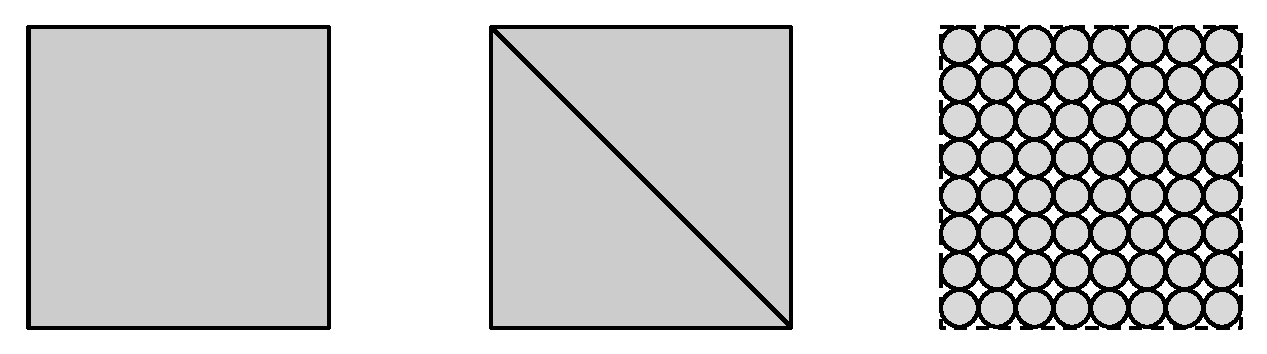
\includegraphics[scale=0.6]{figures/pol_comp.pdf}
	\caption[Modeling types comparison]{
		From left to right; mathematical representation of a plane, representation using two polygons (triangles) and a point-based representation.
	}
	\label{poly_comp}
\end{figure}

Using point based representations, the polygonal approximation step can be skipped and the massive amount of captured data is directly used.

All of these concepts will be explained in depth in their corresponding chapters. 

\section[Motivation and context]{
	Project motivation and context
}

Lately, 3D acquisition systems (commonly known as LIDAR\footnote{\textit{Laser Imaging Detection And Ranging}}) have evolved causing a revolution in work methodologies of several disciplines, from civil engineering, architecture, cultural heritage, movies to videogames. These systems use ultraviolet, visible or near infrared light to image objects. It can target a wide range of materials and even single molecules. A narrow laser beam can map features with very high precision.

Each sample obtained will possess coordinates (x,y,z), color, normal, temperature, etc. This information can be used to obtain measurements, calculations, etc. without having to repeat the capture process again each time we want to measure something new already present in the dataset. This presents clear advantages compared to the classical work-flow of a topographer that would have to measure on site each time a new measurement is required.       

PCM \cite{PCM} is a software library developed by the UDC\footnote{\textit{University of A Coru�a}} for the management of big point datasets obtained using LIDAR. PCM includes basic memory hierarchy management, making it possible to transfer the point cloud data between secondary memory (HDD) and video memory in the graphics card. PCM includes a very basic visualizer, that has the potential to become the seed for a more advanced point cloud software tool that will allow the user to access all of these features in real-time.   

Because of the massive nature of these datasets (some of them possess more than a billion points) achieving real-time manipulation of them is a complex task. It will require the improvement of PCM and a careful performance analysis. Having a system that is able to deal with these amounts of data, will let the user take advantage of the full precision of the capture devices if needed. 

Also because of the huge amounts of data, the possibility of using the massive parallel computing power of graphics cards will be explored. The large number of parallel processors can be used to reduce the computation times as much as possible. 

In this project, a complete software tool for visualization, management and manipulation of massive 3D point clouds will be developed. The tool will be multiplatform (GNU/Linux, Windows and MacOS) and will make use of open source software. That is why for the user interface it will take advantage of QT, that has native tools for all the aforementioned platforms. The resulting QT application will let the user access all of the functionality including an advanced and complete 3D visualizer.
   

\section[Objetives]{
	Project objetives
}

The aim of this project is the design and implementation of a point-based multiplatform software tool for interactive visualization, management and manipulation of massive 3D point clouds. 

The application will offer the user the necessary tools to work effectively with this type of datasets, including a 3D visualizer with advanced point-rendering techniques using OpenGL, that will allow real time interaction with one or multiple point clouds. 

From the interface, the user will be able to:     

\begin{itemize}
\item Select different visualization modes for point-based models: multiple cameras, simple and advanced visualization, multi-resolution, etc.
\item Combine different point clouds with tools that enable rotation, translation and scaling of the clouds.
\item Select points in the clouds for working with them.
\item Apply operations to a part of the cloud or the complete dataset. From simple operations like distance measurements to plane or other geometric primitives detection.
\item Export the work done to a standard CAD format, so the tool can be integrated in other workflows. 
\end{itemize}

The developed tool will take advantage of the parallel computing possibilities of the platforms. Either using the GPGPU capabilities of the graphics card with OpenCL or the multiple cores of the CPU. 

PCM will be used as the foundation for this work. PCM is a project in development that offers several low level tools for working with point clouds of arbitrary size in commodity hardware, from which a multi-resolution structure with different levels of cache is highlighted. This final year project will not only extend PCM with the mentioned features, offering a high level tool for the final user, but will also improve the existing source code; paying special attention to performance aspects.

A series of benchmarks will also be implemented that will allow to obtain automatically and autonomously performance information about PCM and the visualization tool, with graphs and reports. This tool will make finding bottlenecks and performance issues easier.

\section[Structure]{
Document structure
}

The document is organized in the following structure.

\paragraph*{Chapter 1.}
Introduction

A brief summary of the work is presented, covering motivation, context and objetives.

\paragraph*{Chapter 2.}
Planification and methodology

We start by describing the planification and methodology used in the project.
 
\paragraph*{Chapter 3.}
Computer Graphics basics

This chapter briefs the basic concepts about computer graphics. How does the camera work and camera types, what are 3D transformations and how a point is represented in 3D.
 
\paragraph*{Chapter 4.}
Structure of a real-time visualizer for point-based datasets

This chapter describes the structure of the visualizer and presents the class diagram of the software.

\paragraph*{Chapter 5.}
PCM

The chapter explains what is PCM and what improvements were made to the library.

\paragraph*{Chapter 6.}
ToView

In this chapter we detail everything related to ToView, the software package developed from scratch in this project.

\paragraph*{Chapter 7.}
Advanced GPU point rendering

An in depth analysis of the most advanced point rendering techniques nowadays.

\paragraph*{Chapter 8.}
Object detection: RANSAC

In this chapter, an extensive explanation of the RANSAC algorithms used in this project is given.

\paragraph*{Chapter 9.}
Preprocessing and filtering

A chapter that explores the preprocessing and filtering techniques implemented in the project.

\paragraph*{Chapter 10.}
Conclusions and future lines of work

Finally, future possibilities for the project and conclusions reached during its development are exposed.
 
 





	%
% T�TULO DEL CAP�TULO
%
\chapter[Planification and methodology]{
	Planification and methodology
	\label{chapter_2}
}

This chapter explains what software development method was used in the project. We are strong believers in agile software development, above all for research oriented projects like this. In the next sections, some basic concepts of this development philosophy are introduced, as well as how it was applied in our project. Furthermore, a Gantt chart with the different steps and periods of the development is presented so that the reader can see how long each element of the project took. Since this is a project that requires a lot of research, it is difficult to plan ahead; because we do not know how long we are going to spend on a certain element. Finally we will give a cost table with the estimated project cost.

\section[Agile software development]{Agile software development}

Agile software development \cite{agiledev} is a combination of development methods that use iterative and incremental development, where requirements and solutions mature through collaboration between self-organizing, cross-functional teams. The motto of this method is ``embrace change''; that is why it encourages adaptive planning, evolutionary development and delivery, a time-boxed iterative approach, and promotes quick and flexible response to change.

\subsection[Agile manifesto]{Agile manifesto}

In February of 2001, several developers met at Snowbird, Utah resort, to debate different lightweight development methods. They published the \emph{Manifesto for Agile Software Development} \cite{agilemani} to define the approach that is now called agile software development. 

The conclusions that we can reach from the manifesto's items are described below:

\begin{itemize}
\item \textbf{Individuals and Interactions}: In agile development self-organization and motivation are really important. Other values promoted by the manifesto are co-location\footnote{The act of placing multiple individuals within a single location.} and pair programming\footnote{Two programmers work together at one workstation.}.
\item \textbf{Working software}: Working software will be utilized for more purposes than presenting documents to the client.
\item \textbf{Customer collaboration}: The software requirements cannot be fully realized from the beginning of the software development cycle, so being in touch with the customer is really important.
\item \textbf{Responding to change}: Agile development is keen on fast responses to change and continuous development.  
\end{itemize}

More principles are mentioned in the manifesto, some of them are:

\begin{itemize}
\item Customer satisfaction by rapid delivery of useful software.
\item Welcome changes even late in the development.
\item Working software is the principal measure of progress.
\item Maintaining a constant pace.
\item Cooperation between business people and developers. 
\item Build projects around motivated individuals.
\item Attention to technical excellence.
\item Simplicity.
\end{itemize}

Agile methods break down task into small increments with minimal planning and normally long-term planning is not directly involved. \emph{Iterations} are short timeframes that typically last from one to four weeks. A team works in each iteration through a full software development cycle; including planning, requirements analysis, design, coding, etc. This minimizes risk and facilitates adaptation to change. An iteration may not add enough new functionalities to warrant a market release, but the objective is to have an available release at the end of each iteration. 

Team composition does not depend on corporate hierarchies or corporate roles of team members. They normally have the responsability of completing tasks that deliver the required functionalities that an iteration requires. How to meet an iteration's objectives is decided individually.

The ``weight'' of the method depends on the type of project, the planning and order of tasks in a generalist project should not be the same as in a research project.  

Agile methods encourage face-to-face communication instead of written documents if possible. Most teams work in an open office (the \emph{bullpen}), which makes this type of communication easier. 

Each agile team contains a customer representative, that ensures that customer needs and company goals are aligned. 

Most agile methods encourage a routine that includes daily face-to-face communication among team members. In a brief session team members tell each other what they achieved the previous day, what they are going to do today and the problems that have appeared. 

As agile development emphasizes on working software as the primary measure of progress and has a clear preference in face-to-face communication this results in less written documentation than other methods. This does not mean that documentation should be disregarded, but that less emphasis is made on documentation because is not needed as much.

\subsection[XP]{Extreme programming}

Extreme Programming Explained \cite{XP} describes this method as a software-development discipline that lays out how to organize people to produce higher-quality software more productively.

XP tries to reduce the cost of requirement volatility by using short development cycles, rather than a really long one. In this teaching, change is inherent, inescapable and a desirable aspect of development projects, should be welcome with open arms and planned for in advance, instead to trying to cling to certain fixed requirements.  

Extreme programming also introduces a number of basic values, principles and practices on top of the agile programming principles.

\begin{itemize}
\item \textbf{Values}
	\begin{itemize}
		\item \textit{Communication:} To build a software system it is required to communicate the requirements to the developers. This is achieved through documentation.
		\item \textit{Simplicity:} It is encouraged to start simple and add extra functionality at a later time. The main difference between this method and others is focusing on design and coding that satisfies the needs of today and not tomorrow.
		\item \textit{Feedback:} From the system, customer and team. This is closely related to communication and simplicity.
		\item \textit{Courage:} Simplicity, refactoring and getting rid of code when necessary require courage.
		\item \textit{Respect:} Respect for others and yourself. Always think of the team when making changes and respect the work of everybody.
	\end{itemize}
	\item \textbf{Principles}
	\begin{itemize}
		\item \textit{Feedback:} This principle is most useful when is done frequently and promptly. Minimal delay between actions and feedback is key to learning and making changes.
		\item \textit{Assuming simplicity:} The fact of treating every problem as if its solution were really ``simple''. This doctrine stresses that big changes all at once do not work.
		\item \textit{Embracing change:} Change should be embraced instead of trying to work against it or avoid it.
	\end{itemize}
	\item \textbf{Practices}
	\begin{itemize}
		\item \textit{Informative workspace:} Build your workspace around your work. Anyone that visits your workspace should have a general idea of how the project is going in 15 minutes.  
		\item \textit{Sustainable pace:} Work as many hours as you can be productive. Overworking today and wasting the next two days is not good.
		\item \textit{User stories:} Plan using units of work that the client will understand. Having the stories on display will help with having an informative workplace and keeping track of progress. 
		\item \textit{Incremental design:} Invest in system design every day. Try to excel in designing the system so that it meets the day to day requirements.
		\item \textit{Pair programming:} A technique in which two programmers work together in a single workstation. 
		\item \textit{Continuous integration:} This technique helps to prevent integration problems. It consists on merging all developer working copies with a shared stable version of the software. 
		\item \textit{Ten minute build:} Build the complete system automatically and execute every test in 10 minutes. 
		\item \textit{Test-driven development:} Write automatic tests that fail before changing any code.
		\item \textit{Whole team:} Not only the developers should communicate between each other, the customer should also be available for questions.
		\item \textit{Sit together:} Have an open space available for the team. If it is not possible, video-conferences should be used to have more face to face time.
		\item \textit{Weekly cycle:} Start the week writing automated tests and then during the week implement them. 
		\item \textit{Quarterly cycle:} Plan for releases that will cover themes. Themes are broken down into stories for weekly cycles.  
	\end{itemize}
\end{itemize}

\subsection[Application]{Application}

We have used in our project several of the premises of agile software development. We have used approximately weekly or biweekly iterations focused on completing simple objectives that would yield working software. The work in each iteration has been constant and diligent, focusing always on completing the task at hand, but not avoiding changes if it was deemed necessary. 

Also several XP practices were used in the project. Such as user stories (see \figurename~\ref{story_cards}), were each planned functionality was broken up in stories if big enough. Then the effort to implement each story was estimated directly since the estimation units are simple enough to provide a rough estimate, but because of the nature of the project this estimates were not very precise even when estimating just small units. They were just meant as guidance and mainly used to keep track of progress.  Another practice followed was an informative workspace, the story cards were stuck to the wall so they were easily visible to everybody. They were also organized in groups, so the progress in each functional area was easily tracked.

\begin{figure}[h]
	\centering
	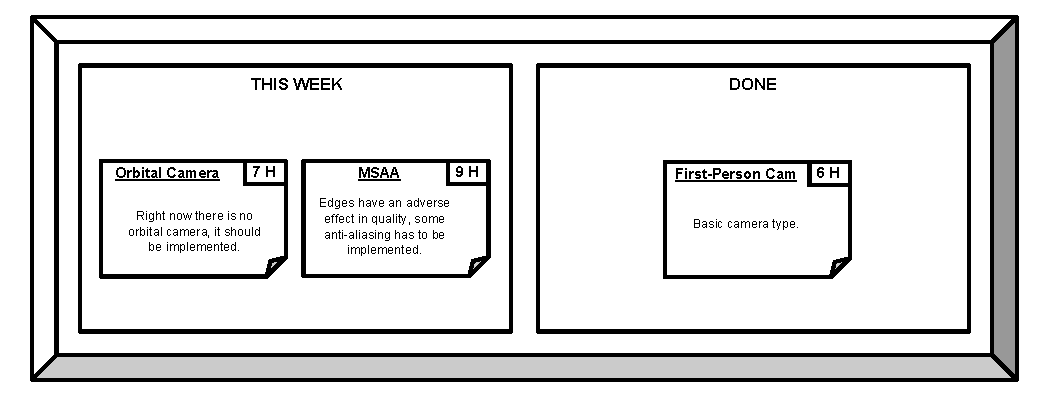
\includegraphics[scale=0.6]{figures/story_cards.pdf}
	\caption[Story cards]{
		In this image we can see a sketch of the structure of a story card and how they were organized.
	}
	\label{story_cards}
\end{figure}

Incremental design was also used, every day the design was reviewed and adapted to the new requirements. Lastly, a sustainable pace was kept. Because designing and implementing software is a creative process that requires insight, developers have to be rested, ready and motivated. To make the most of the worked time, the premise of coding for two hours straight without checking e-mails or other distractions was used, along with other similar productivity tricks. 

The meetings with my two advisors were kept on face-to-face basis when possible. In each meeting we would comment what had been achieved since the last one, laid out what the objectives were for the next iteration and talked about the roadblocks found on the task at hand. Whenever communication in person was not possible, e-mails were exchanged regularly if tasks where completed or any other event arised. 

To keep the code accessible by everyone in the team, up to date and well organized \textbf{Git} \cite{gitrev} version control software was used. Git is free software used to manage source code and keep distributed revision control. Every Git working directory is a repository with complete history and revision tracking capabilities. In this project it was essential to have a system like this in place, because of the research nature of the project. Ideas needed to be tried without wasting time on keeping tabs on the added code, Git makes this really easy and not problematic thanks to history and revision tracking.

Since the project is divided in two sub-projects (PCM and ToView\footnote{The visualizer, the main focus of this project.}), it was also necessary to manage the separate repositories in some way. With this in mind, \textbf{Redmine} \cite{redmine} was chosen to achieve our goal. This is a free and open source web-based tool for project management and bug tracking. It has support for multiple projects, a Gantt chart, calendar, support for multiple users, several types of repositories, news, wiki, etc. 

As this project is meant to be open source, this tool will allow the coordination of the efforts of future developments well after the end of this project. We believe this project will be a good fit for the ``bazaar type'' of development that other successful open source software has used. In this model, the code is developed openly for everyone to see. This type of development also encourages the participation of the user in the development process.      

We have also estimated the cost of the project as we can see in Table~\ref{cost_table}. It only includes human resources and hardware costs because all the software used was free.

\begin{table}
\begin{center}
\begin{tabular}{lcccr}
\toprule
Resource & Units & Hours & Cost per hour & Total \\
\midrule
  Software &  &   &  & 0 \euro \\
  Computer & 1 &   &  & 1800 \euro \\
  Analyst-programmer & 1 & 950 & 16 \euro & 15200 \euro \\
  \midrule
  &&&&17000 \euro\\
\bottomrule
\end{tabular}
\end{center}
\caption[Cost estimate]{
		Table showing the estimated cost of the project.
}
\label{cost_table}
\end{table}

Although because of the research nature of the project it was not possible to estimate how much time we would spend in each iteration, we provide a Gantt chart that depicts how the project iterations were performed after the fact (see \figurename~\ref{gantt_chart}).

\begin{landscape}
	\begin{figure}
		\centering
		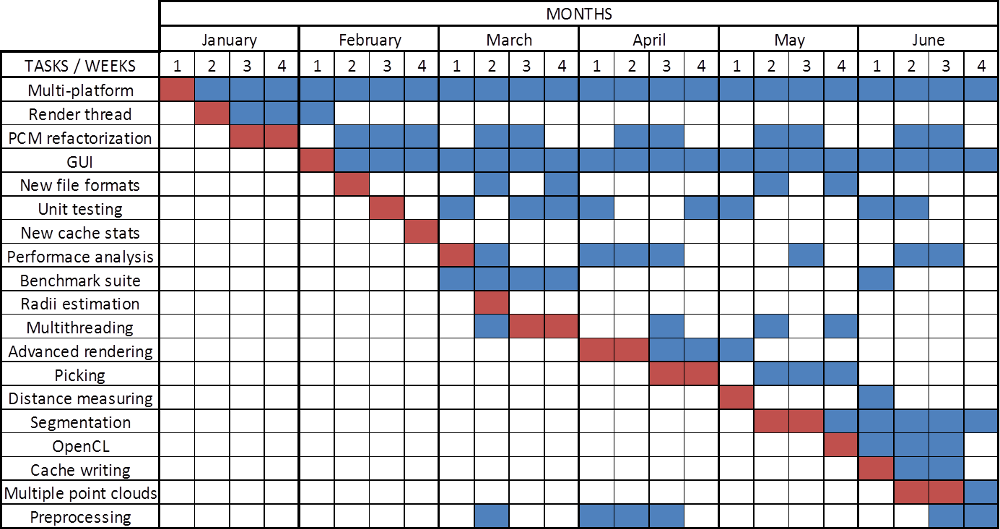
\includegraphics[scale=0.6]{figures/gantt.png}
		\caption[Gantt chart]{
			Gantt chart of the project.
		}
		\label{gantt_chart}
	\end{figure}
\end{landscape} 
















	%
% T�TULO DEL CAP�TULO
%
\chapter[CG basics]{
	Computer Graphics basics
	\label{chapter_3}
}

In this chapter, some concepts in 3D rendering are introduced, paying special attention to the main components of a real time point-based rendering visualizer. We first describe the process that generates the frame-buffer. This means that we have to explain the camera model. We will also depict how we represent points in space by several means that will be introduced in this chapter.

Only a brief description of these concepts is presented, to get more familiarized with Computer Graphics the book \cite{CGPP} is recommended. For point-based rendering techniques the book \cite{pbg} is an essential source.

\section[Rendering]{
	Rendering
}

Traditionally Computer Graphics has been defined as the computer science discipline that is dedicated to synthesizing images algorithmically with computers. Nowadays we can find even more related topics like hyper realistic photography, animation techniques, virtual reality, etc. To generate images from three-dimensional scenes a process called \textbf{render} is used. This set of actions  is in charge of modeling objects and their properties, illumination if needed and the camera that will capture everything.

As has been said before, rendering is the computational process of generating an image from a model. From this definition multiple interpretations are possible, from creating a 3D animation film to a bar chart in a spreadsheet, all of them are equally valid. Although the term is normally used when the model we are using is of a spatial nature and more specifically three-dimensional.

Several classifications of rendering techniques could be made, but for this introduction we will use two of them. On one side, if we use the type or style of the image we want to achieve, we will have:

\begin{itemize}
\item \textbf{Non-photorealistic rendering}, uses other types of effects that render the scene with artistic style, intended to look like a painting or drawing.
\item \textbf{Photorealistic rendering}, tries to be as faithful as possible to reality. This type of render can be subdivided in: 
	\begin{itemize}
	\item \textbf{Physically-based rendering}: Tries to compute an authentic simulation of light transport through the virtual scene and its interaction with materials and objects. The precision of this simulation will depend on the mathematical and physical models chosen.
	\item \textbf{Faked}: Utilizes algorithmic tricks, not trying to pretend an ad-hoc simulation of light, usually to reduce render times.  
	\end{itemize}
\end{itemize}

\begin{figure}[h]
	\centering
	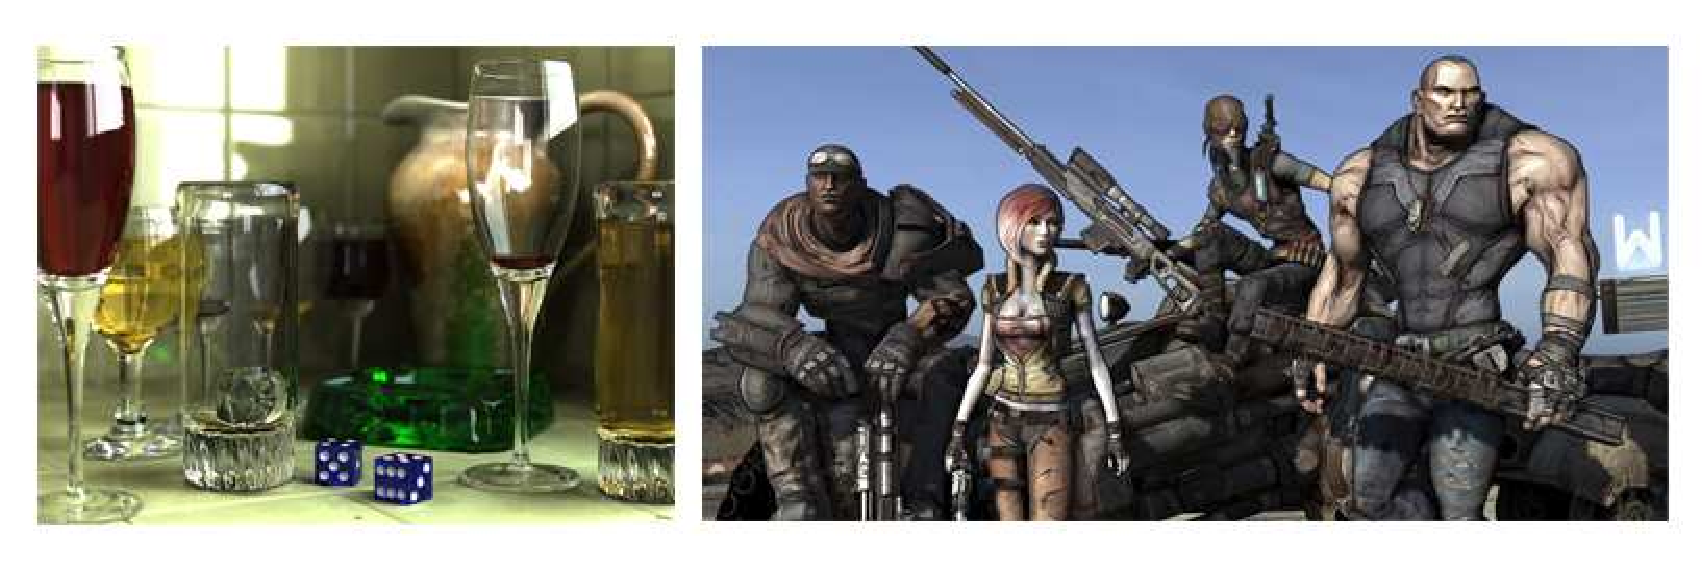
\includegraphics[scale=0.5]{figures/photo_comp.pdf}
	\caption[Rendering types comparison]{
		A photorealistic render on the left, versus a non-photorealistic render on the right.
	}
	\label{photo_comp}
\end{figure}

On the other side, if we compare the interaction capabilities of the rendering application with the user, we can divide rendering techniques in: 

\begin{itemize}
\item \textbf{Offline rendering}: Where the process that generates the image is too slow to respond instantaneously to the user interactions. A time scale of seconds and up to several days can be considered ``slow''. This happens for example when generating photograms for a movie.
\item \textbf{Online rendering}: Where processing time would be short enough to respond to user interactions so that the user has the sensation of continuity. A time scale of miliseconds would be needed to achieve this effect. Normally it is measured in \emph{frames per second} (FPS). A good example of this technique are videogames. 
\end{itemize}

Almost everything in this document will be devoted to non-photorealistic real-time rendering techniques, since ToView is aimed as way for the user to interact in real-time with massive point clouds.

For more information about real-time rendering please consult \cite{realtime}.

\subsection[Rendering process]{Rendering process}

There are several techniques for generating images from a model. All of them start with a camera position, the geometry of the objects is projected in that direction one way or another, calculating the color of each resulting pixel. The two families of techniques are the ones based on \emph{scanline rendering}, where lists of geometry are traversed with horizontal scan lines. Intermediate calculations determine what object is closer to the camera, how do the lights in the scene affect the objects, etc.

Since we require real-time rendering, we will take advantage of the power of the GPU. The GPU \textit{pipeline} is the process implemented in hardware to create images from the scene information in a highly efficient way. It is comprised of several stages were several lineal algebra operations that account for the position, rotation and scaling of the point of view, objects and lights; to finally determine the color of the pixel drawn to the screen. 

A GPU can be used to process graphical data using two APIs\footnote{\textit{Application Programming Interface}}:

\begin{itemize}
\item \textbf{DirectX}: Microsoft's propietary API, only useful in Windows systems. 
\item \textbf{OpenGL}: Standard and multiplatform, this were the main reasons why it was the chosen API for this project. 
\end{itemize}

\begin{figure}[h]
	\centering
	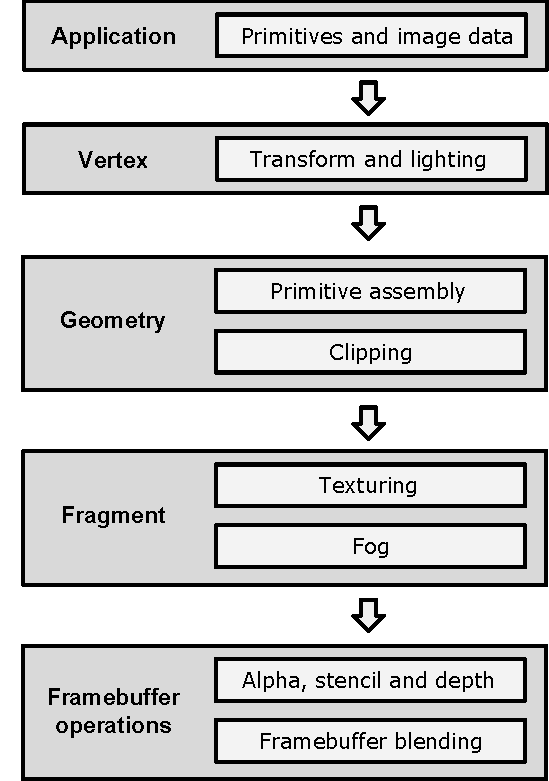
\includegraphics[scale=0.6]{figures/ogl_pipe.pdf}
	\caption[OpenGL pipeline]{
		The OpenGL pipeline.
	}
	\label{opengl_pipe}
\end{figure}

In modern GPUs, some of the stages of the pipeline can be modified using small programs written in GLSL\footnote{\textit{GL Shading Language}} called shaders. In \figurename~\ref{opengl_pipe} the simplified pipeline of a modern version of OpenGL can be observed. In it the vertex, geometry and fragment stages are programmable. The \textit{frame-buffer}\footnote{The portion of memory (buffer) reserved to maintain temporally an image (frame) awaiting to be sent to the monitor.} will be the final image that will be shown onscreen. 

Although there are some constraints in the form of number of instructions and control structures, shaders started a revolution in real-time rendering. Sometimes even allowing to create images almost as realistic as offline rendering.  

\subsection[Models]{
	Models
}

Modeling describes the process of forming the shape of a virtual object in a computer. There are several types of models (see \figurename~\ref{model_comp}):

\begin{itemize}
\item \textbf{Polygon-based}: Describe the surface of an object as a set of polygons. Triangles are the most commonly used polygons, since they are flat and trivially convex. Most of the existing graphics hardware is optimized for this primitive.
\item \textbf{Voxel-based}: Divides space in a regular 3D grid where the \emph{voxel} is the smallest unit of volume. Each cell is either filled or not and depending on that the pixels are shaded. Memory increases as precision is augmented. 
\item \textbf{Point-based}: Objects are represented by point samples of their surface, that is why they are usually called \emph{splats}. Each point has a position and some information about the surface that it belongs to. Compared to the traditional triangle-based approach, this primitive needs its own rendering techniques and its own pipeline, since different challenges must be faced. This is our case study and because of that, this primitive will be further explained in Section~\ref{splats_and_points}.
\end{itemize}

\begin{figure}[h]
	\centering
	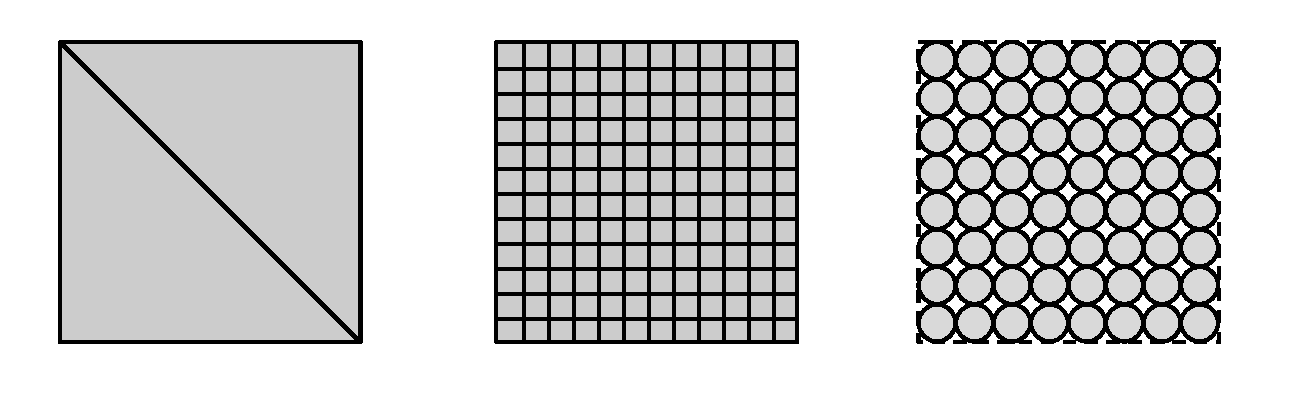
\includegraphics[scale=0.6]{figures/model_comp.pdf}
	\caption[Model types comparison]{
		From left to right; a polygon-based, a voxel-based and a point-based model of a plane (2D representation).
	}
	\label{model_comp}
\end{figure}

%
% SECCION - T�tulo de la secci�n
%
\section[Splats]{\label{splats_and_points}
	Splats and points
}

A point cloud is a set of vertices or points in a three-dimensional coordinate system. These vertices are usually positioned in 3D space and have a set of coordinates $(x,y,z)$. These sets of points normally are representative of the external surface of an object. 

\begin{figure}[h]
	\centering
	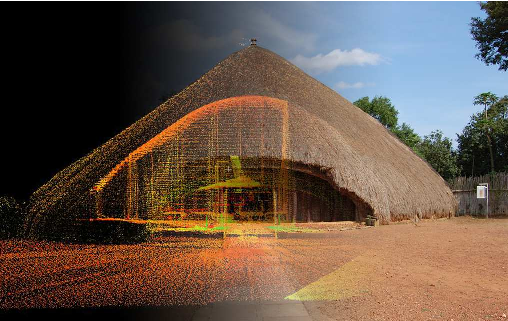
\includegraphics[scale=1]{figures/point_cloud.pdf}
	\caption[Point cloud]{
		Photo overlaid atop laser scan data from a project held in early 2009 at Kasubi Tombs.
	}
	\label{point_cloud}
\end{figure}

Point clouds are normally created by 3D scanners, these devices capture automatically a large number of points on the surface of an object (see \figurename~\ref{point_cloud}), and yield a point cloud dataset as a result. 

The points from the range data represent a surface, but a point is zero-dimensional; this means that it does not have volume, area, length or any other higher dimensional equivalent. Usually point clouds are not directly usable in most 3D applications because of this reason. That is why we need splats (surface elements), that describe the surface in a small neighborhood. 

At this point we need to choose how the surface will be represented by the point. In our project we will represent the splat as a disc. 

\begin{figure}[h]
	\centering
	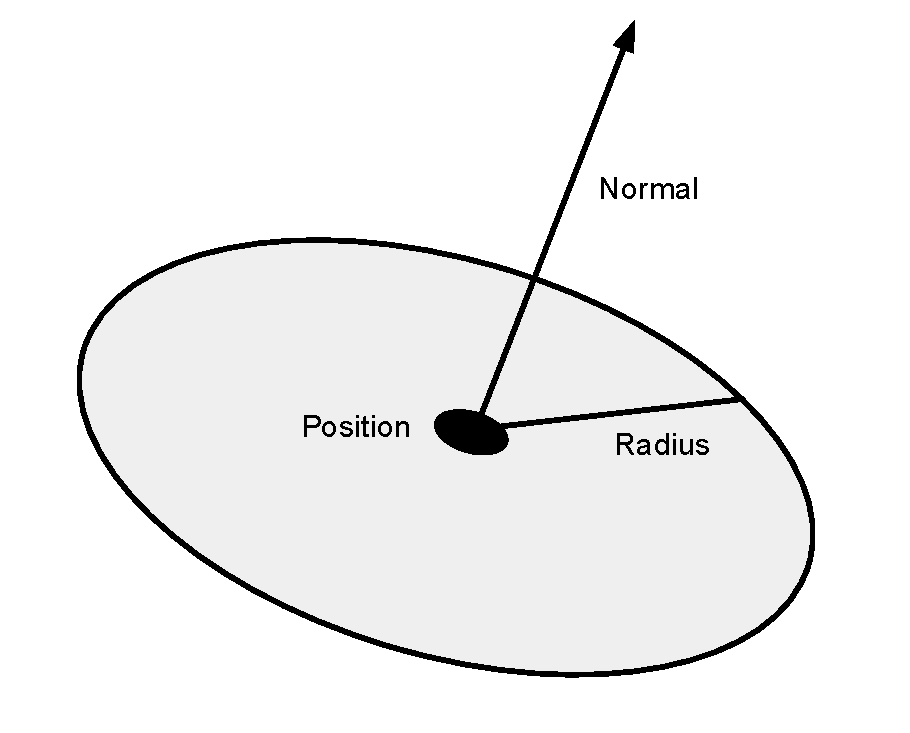
\includegraphics[scale=0.4]{figures/surf_disc.pdf}
	\caption[Disc approach]{
		Visual representation of the splat as a disc.
	}
	\label{surf_disc}
\end{figure}

If on the other hand we choose to represent the splat as a disc, the splats can have have the following parameters (see \figurename~\ref{surf_disc}):

\begin{description}
  \item [Position:] \emph{x}, \emph{y} and \emph{z} coordinates in world space.
  \item [Normal:] A vector that represents the surface normal of the splat. It can be provided or the engine can estimate it.
  \item [Radius:] This will be the radius of the sphere that will represent the splat. The engine will also be capable of calculating the radius automatically.
  \item [Color:] The splat color in RGB parameters if we are going to use the lighting from the scanned data.
  \item [Other properties:] Intensity, reflectivity, temperature, etc.
\end{description}

\section[Transformations]{
	3D Euclidean space and transformations
}

In 3D computer graphics we normally work with a three-dimensional space of Euclidean geometry, the term ``Euclidean'' is used to distinguish between these spaces and the curved spaces of non-Euclidean geometry. The most common types of operations in Euclidean geometry can be represented with a transformation matrix if homogeneus coordinates are used. Because of this a transformation \textbf{T} can be used for several purposes. 

Using basic linear algebra concepts, a $4\times4$ matrix can be used to express the linear transformation of a point or vector. A transformation will then be represented by the elements of the $4\times4$ matrix. They can also be used to perform some transformations that are non-linear on an Euclidean space. For this reason transformation matrices are widely used in computer graphics.

Generally a transformation is a mapping from points to points or vectors to vectors \cite{PBRT}, for example: \begin{equation}p' = \textbf{T}(p) \;\;\;\;\; v' = \textbf{T}(v)\end{equation} 

To transform the points or vectors we just have to perform the appropriate matrix multiplications. This also allows the composition of transformations, we just have to multiply the transformation matrices. 

Most commonly used transformations are:

\begin{itemize}
\item \textbf{Rotation}, will rotate a point or a vector by a given angle either around an arbitrary axis or the $x$, $y$ or $z$ axis.
\item \textbf{Scaling}, takes a point or a vector and will scale its $x$, $y$ and $z$ components by a factor.
\item \textbf{Translation}, only affects points and will translate coordinates $x$, $y$ and $z$ a set amount.
\item \textbf{Model}, this matrix is useful for transforming the model locally. It is comprised of a set of rotation, scaling and translation matrices. When we apply this matrix to all the points, we will have them in world coordinates.  
\item \textbf{View}, initially the camera is placed in the origin of world space. To be able to move around the world this transformation is used. This matrix is also called \textit{look-at}. After this transformation is applied, we will have the points in camera coordinates.
\item \textbf{Projection}, since a 3D scene has to be projected onto the screen as a 2D image, we need another process that converts the points from camera coordinates to homogeneous coordinates so that they can be projected onscreen. 
\end{itemize}

Usually the composition of the model, view and projection matrices is called \textit{MVP} and is applied to every point that we want to draw.

To illustrate how the transformations are represented by a $4\times4$ matrix, equation~\ref{eq_trans} shows the generic transformation matrix for a translation: \begin{equation}\label{eq_trans}\textbf{T}(\Delta x,\Delta y,\Delta z) = \begin{pmatrix}
 1& 0 & 0 & \Delta x\\ 
 0& 1 & 0 & \Delta y\\ 
 0& 0 & 1 & \Delta z\\ 
 0& 0 &0  & 0
\end{pmatrix}\end{equation}

This transformation is applied to a point $P=(x,y,z)$ in the following way: \begin{equation}\begin{pmatrix}
 1& 0 & 0 & \Delta x\\ 
 0& 1 & 0 & \Delta y\\ 
 0& 0 & 1 & \Delta z\\ 
 0& 0 & 0 & 0
\end{pmatrix} \begin{pmatrix}
x\\
y\\
z\\ 
1
\end{pmatrix} = \begin{pmatrix}
x+\Delta x\\
y+\Delta y\\
z+\Delta z\\ 
1
\end{pmatrix}\end{equation}

\section[Camera model]{
	Camera model
}

Almost everyone nowadays has used a camera and knows its basic purpose: you want to record an image of the world (usually pressing a button) and the image is then recorded on a film. One of the simplest  cameras in the real world is the \emph{pinhole camera}. Pinhole cameras use a light tight space with a hole at one end. When this hole is uncovered light enters through the hole and reaches a piece of photographic paper on the other end of the box (see \figurename~\ref{pinhole}). In this day and age, cameras are more complex than this simple camera model, but this is a good starting point to explain how our simulation works.

\begin{figure}[h]
	\centering
	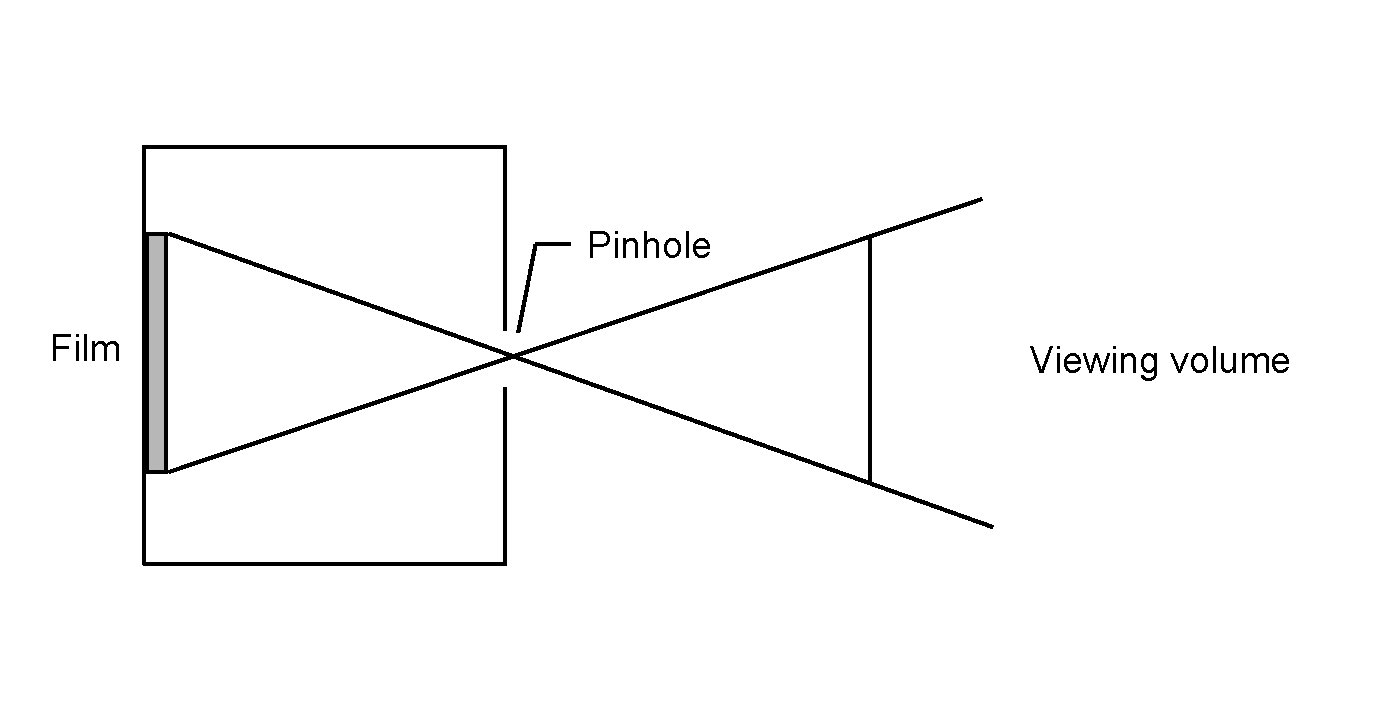
\includegraphics[scale=0.5]{figures/pinhole.pdf}
	\caption[Pinhole camera]{
		Diagram explaining how a pinhole camera works.
	}
	\label{pinhole}
\end{figure}

The most important function of the camera is defining the part of the scene that will be recorded on the photographic film. Connecting the pinhole to the edges of the film creates a double pyramid that extends into the scene. Objects that are not inside this pyramid will not be imaged on the film. As cameras are now more complex, we will refer to the region that can be imaged as \emph{viewing volume}. 

If we were to use the pinhole as the film, the viewing volume would not change. When the film or image is infront of the pinhole, the pinhole is frequently referred to as the \emph{eye}. In our simulated camera where the film is infront of the eye, we will display the amount of light traveling from the image plane to the eye. Several tests will be performed by OpenGL depending on the type of camera to check which points can be seen and have to be represented in the frame-buffer. 

The camera model used in this project supports several settings. First we explain how this settings affect the camera model, after we detail how the camera model interacts with the ray tracing process. Readers can consult \cite{PBRT} if they want to delve deeper in the topic.

\subsection[Parameters]{Camera parameters}

The first parameter that the camera model supports is \textbf{camera position}. This parameter states where the camera will be positioned in world space coordinates (\emph{x,y,z}).

Next supported parameter is the \textbf{camera orientation}. This parameter is a point in the world at which the camera is looking at.

\begin{figure}[h]
	\centering
	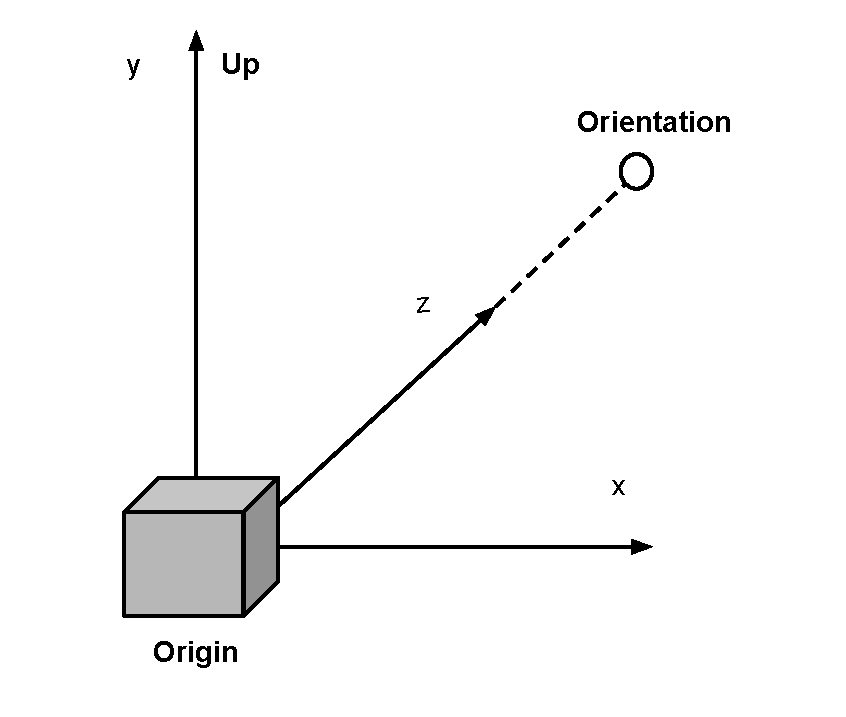
\includegraphics[scale=0.55]{figures/cam_ori.pdf}
	\caption[Camera orientation]{
		Diagram explaining the camera coordinates.
	}
	\label{cam_ori}
\end{figure}

We also need to know how to orient the camera along the viewing direction implied by the first two parameters. The parameter \textbf{camera up vector} gives us that orientation. 

We can see how this parameters are organized in camera space in \figurename~\ref{cam_ori}.

Other important parameters in a camera model are the clipping planes. \textbf{Hither} dictates where the near clipping plane of the camera is located and \textbf{yon} indicates where the far clipping plane is situated as we can see in \figurename~\ref{hither_yon}. The camera's clipping planes give us the range of space along the \emph{z} axis that will be visible in images. Objects that are in front of the hither plane or beyond the yon plane will not be visible. 
\begin{figure}[h]
	\centering
	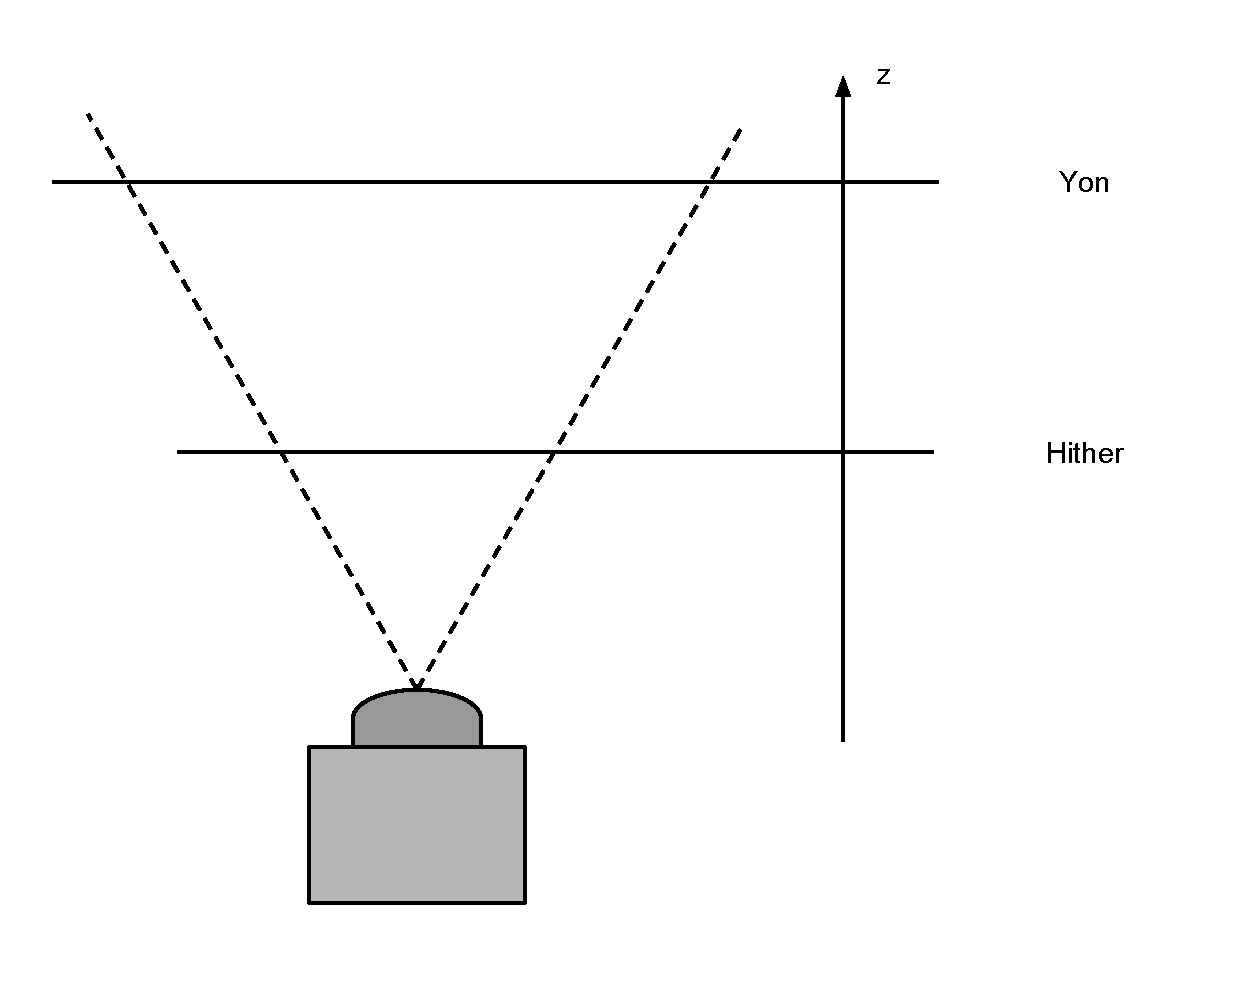
\includegraphics[scale=0.5]{figures/hither_yon.pdf}
	\caption[Hither and Yon]{
		Representation of hither and yon planes.
	}
	\label{hither_yon}
\end{figure}

The last parameter that the camera supports is the \textbf{field of view}. The angle of view describes the angular extent of the scene captured by the camera horizontally and vertically. 

The clipping planes and the angles of view define the viewing volume in our model, also known as the \emph{viewig frustum} (see \figurename~\ref{frustum}).

The user also has the option to use a \textbf{perspective} or \textbf{orthographic} camera depending on what his needs are. An architect for example may prefer an orthographic camera, while a normal user may use a perspective camera that will yield a more natural image as result. 

Orthographic projection is more commonly used in engineering because dimensions are communicated unambiguously, if there is a one unit length line anywhere in the scene; it will appear the same length everywhere. Also every line that is parallel in the scene will be parallel in reality. With perspective projection, lines of identical real-world length will appear different due to \textit{foreshortening}\footnote{Objects becoming smaller on the image plane as they get further away.}. This is why it will be difficult to judge relative dimensions when objects are far away.

Another option that is available is using a \textbf{FPS}\footnote{First-Person Camera} or an \textbf{orbital} camera. On one hand with a first person camera the user can walk freely just like if he was inside the scene, forward, back, left, right, etc. On the other hand with an orbital camera the user sets a center point and then orbits around said point.     

\subsection[Inner workings]{Camera inner workings}

Once we have the camera parameters we need to place the camera in the scene, we will use a \emph{look-at} transformation for this purpose. Using the look-at transformation as view matrix will give us a transformation between world and camera coordinates as mentioned before. The next step will depend on the type of camera that the user will choose, either orthogonal or perspective. In light of this a projection matrix will be chosen reflecting the choice. The composition of these matrices will yield the MVP matrix. This is the mathematical expression used for transforming each point:

\begin{equation}\begin{split}v' & = \textbf{\textit{P}}\cdot \textbf{\textit{V}} \cdot \textbf{\textit{M}} \cdot v \\ & = \textbf{\textit{MVP}} \cdot v\end{split}\end{equation}    

Once we have the MVP matrix, we can perform \emph{frustum culling}. The visualizer selects the only the points that fall inside the \emph{viewing frustum} (see \figurename~\ref{frustum}). This is a essential process to achieve the necessary performance to be able to render the point clouds in real-time. The viewing frustum is the region of space that will appear in the images generated by the visualizer. This process of eliminating objects that are outside the viewing frustum is called \emph{viewing frustum culling}.

\begin{figure}[h]
	\centering
	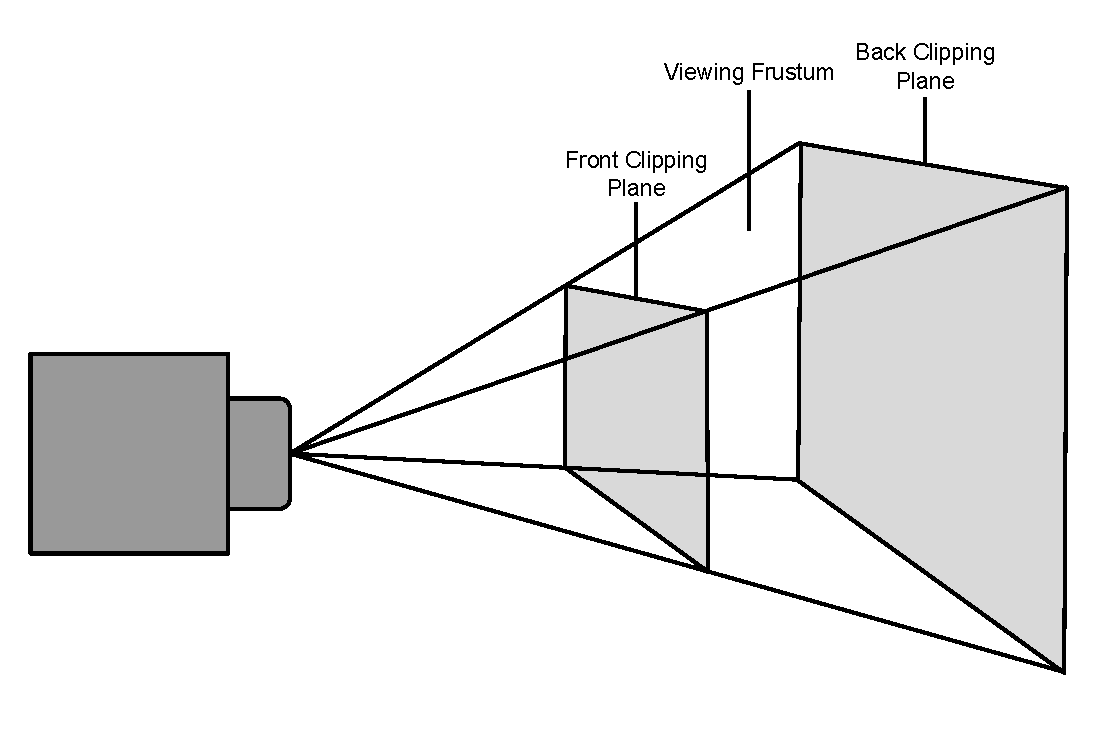
\includegraphics[scale=0.55]{figures/frustum.pdf}
	\caption[Viewing frustum]{
		Diagram showing the viewing frustum.
	}
	\label{frustum}
\end{figure}

These computations are costly when the scenes are big and to simplify the culling process we need an acceleration structure. These structures reject chunks of the scene that are not inside the frustum. In our project we have chosen to use a multi-resolution \emph{k-d tree}.

If an orthographic transformation is used, points will be projected to the far viewing plane. This type of transformation does not give the effect of foreshortening, it keeps lines parallel and preserves relative distance between objects. This transformation leaves \emph{x} and \emph{y} coordinates unchanged, but maps \emph{z} values at the hither plane to 0 and \emph{z} values at the yon plane to 1.

Once we have the adequate coordinates we just have to map them to screen space depending on the resolution of the render. If two points are mapped to the same pixel we have to see which one is closer in the \emph{z} axis, because that will be the point that the pixel is going to represent.

\begin{figure}[h]
	\centering
	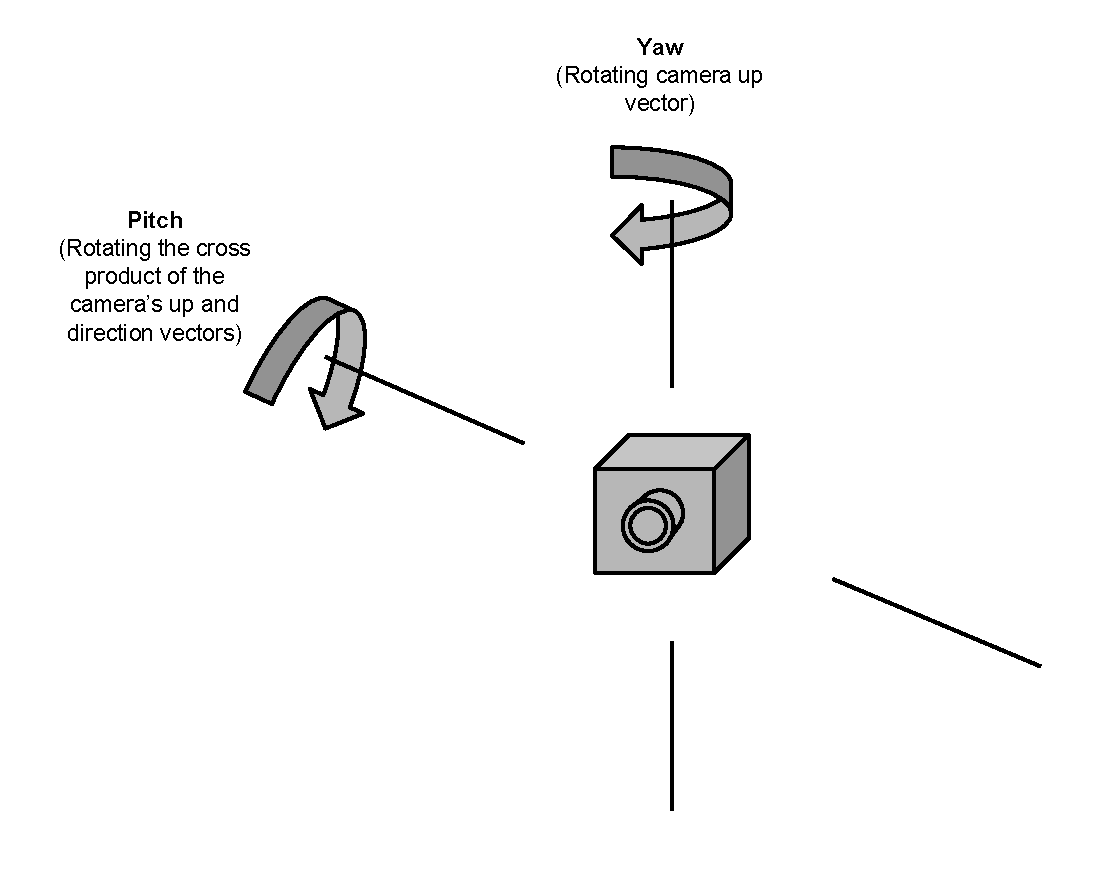
\includegraphics[scale=0.5]{figures/cam_rotation.pdf}
	\caption[FPS camera rotation]{
		Diagram showing the rotation in a first-person camera.
	}
	\label{FPS_rot}
\end{figure}

If on the contrary we chose to use a perspective camera, we have to take into account the foreshortening effect we mentioned before. This projection does not preserve distances or angles, and parallel lines no longer remain parallel. \emph{x} and \emph{y} are not left unchanged, they are modified according to the corresponding \textit{z} value, that dictates how close to the camera the point is.

This is the course of action followed to create one frame, but since the visualizer is interactive, we have to repeat this process several times per second. Furthermore, we have to take into account how the user wants to move. If the FPS camera option is chosen, we start in a certain position and then we will be able to move forward, backward, left and right just as we would be able to do if we were walking around the scene in reality. The user will also be able to look around with complete freedom (see \figurename~\ref{FPS_rot}). \textit{Yaw} allows the user to look left and right and \textit{pitch} up and down.   
 
\begin{figure}[h]
	\centering
	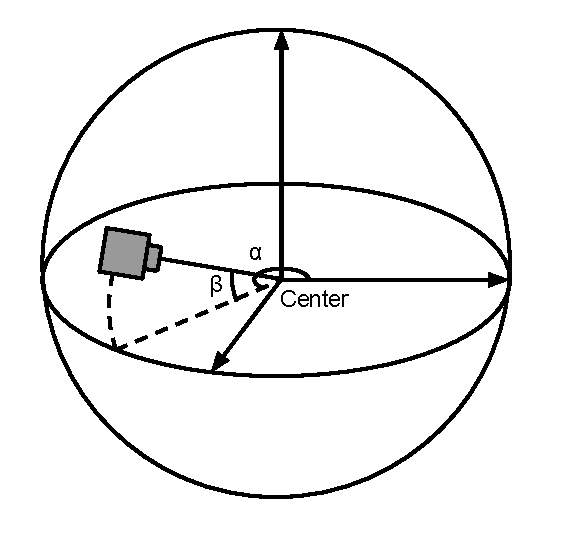
\includegraphics[scale=0.8]{figures/orb_rot.pdf}
	\caption[Orbital camera rotation]{
		Diagram showing the rotation in a orbital camera.
	}
	\label{orb_rot}
\end{figure}

When the orbital camera is used, instead of freely walking around, we orbit around a center point (see \figurename~\ref{orb_rot}). The rotation in this instance is represented by a number of rotation degrees ($\alpha$ and $\beta$) around the $x$ and $y$ axes of a coordinate system centered in the interest point. Instead of moving the camera, we move the point of interest, that will be followed by the camera.  








	%
% T�TULO DEL CAP�TULO
%
\chapter[Structure]{
	Structure of a point-based visualizer
	\label{chapter_4}
}

In this chapter, the structure of PCM and ToView is shown. Thus, a high level description of the pipeline is done, which serves as a summary of the analysis phase for this project. The different stages of the pipeline are thoroughly described in the following chapters. Finally, a class diagram depicts the main design aspects of ToView and the updated version of PCM. 

\section[Analysis]{Analysis}

\begin{figure}
        \vspace*{0.5cm}
                \centering
				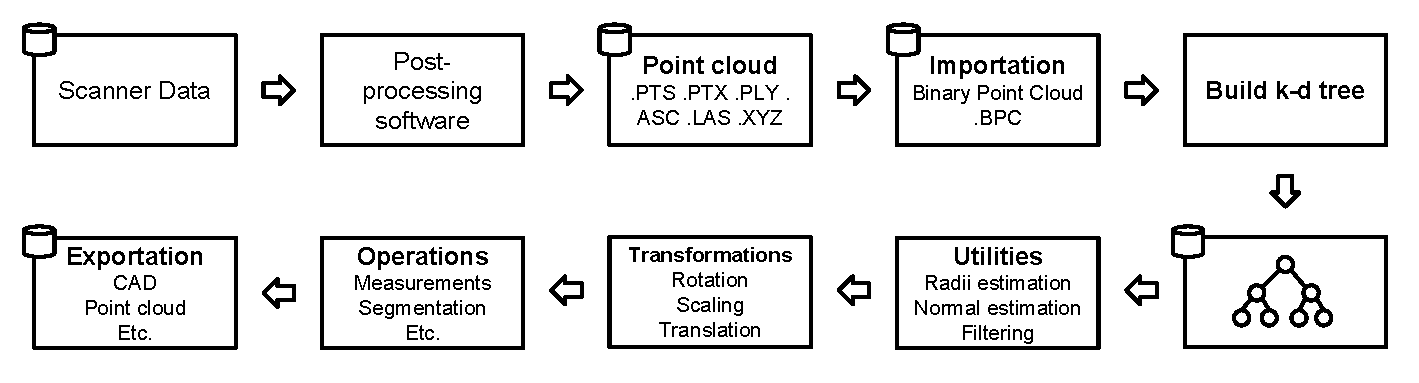
\includegraphics[scale=0.6]{figures/pipeline.pdf}
                \caption[BDE pipeline]{
                        Representation of the usage pipeline of ToView.
                }
                \label{pipeline}
        \vspace*{0.5cm}
\end{figure}

\figurename~\ref{pipeline} depicts the usage pipeline of ToView. To use the system, a series of steps have to be followed. First, the raw LiDAR data is usually processed using software from the manufacturer (unifying scans, calibration, etc.). Once the resulting point cloud from the aforementioned software is available, it will be converted to our point cloud format. 

Next, the k-d tree for accelerating calculations and rendering is created. When the k-d is created and stored in permanent memory, it can be used to estimate radii, normals, apply filters, etc. It can also be used to visualize the point clouds in an efficient way, since we have massive datasets and visualizing them in a naive way is not possible. 

In addition, multiple point clouds can be merged using the visualizer. The user will be able to apply transformations (rotation, scaling and translation) to the individual clouds. This allows the user to for example mix a point cloud that represents a statue with another of its destination, and see in advance how it will look.

ToView can also be used to measure distances in point clouds that were registered with this purpose in mind. Lastly, the visualizer can be used to segment parametric primitives (planes, cylinders and spheres) and export them to a CAD compatible format.        

\section[Design]{Design}
 
ToView is developed following an object oriented approach and using the C++ language \cite{primerplus}. In addition, design patterns have been used as much as possible. The compilers used until now have been Visual C++ 2012 and 2013 in Windows systems and GCC 4 in Linux. For the creation of multi-platform project files, we have made available a CMake \cite{cmake} makefile for PCM and ToView. 

\subsection[Use cases]{Use cases}

Bla bla

\subsection[Class diagram]{Class diagram}

Now that we have exposed the conceptual approach, we show the class diagram of the engine. It will be further explained in the next chapters.

\begin{figure}[h]
                \centering
                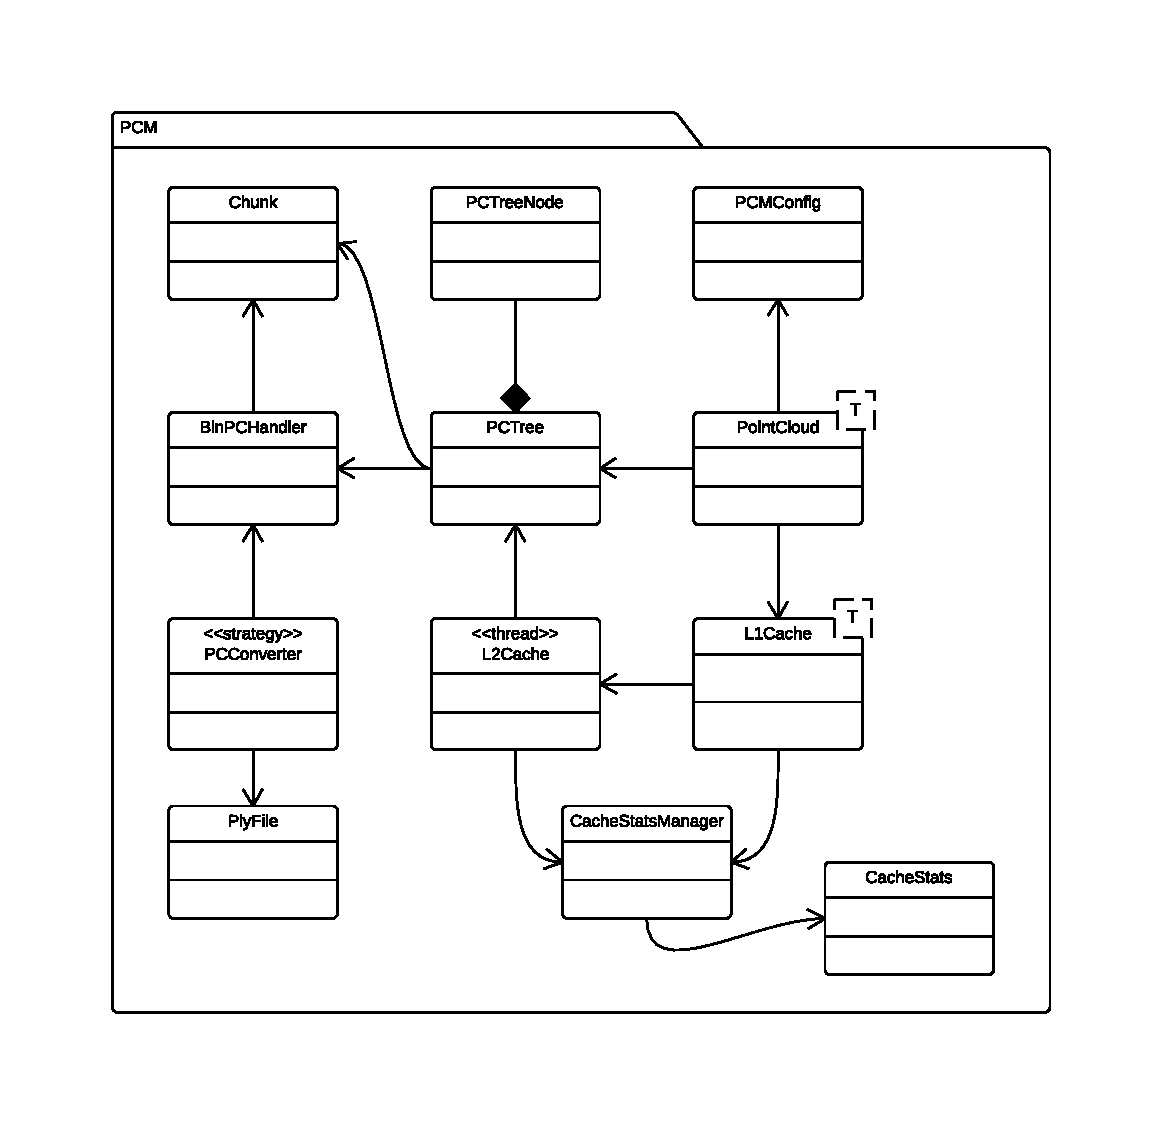
\includegraphics[scale=0.6]{figures/PCM.pdf}
                \caption[PCM class diagram]{
                        PCM class diagram.
                }
                \label{class_dia}
\end{figure}

On one hand we have the library \textbf{PCM} (see \figurename~\ref{class_dia}) that consists of:

\textbf{Chunk} represents the minimum amount of information that will travel across the different levels of memory, that is why its size in bytes will be closely controlled. \textbf{BinPCHandler} is the intermediate compacted format (BPC) in the format conversion process and the spatial structure construction, its objective is representing an arbitrary length array of data that resides in permanent storage. \textbf{PCConverter} is the class in charge of offering a single interface to convert any type of point cloud file.

The spatial structure is represented by \textbf{PCTree}. This class encapsulates two main functionalities, the construction of the chunk database and the multi-resolution tree management and its nodes. \textbf{PCTreeNode} contains information about the nodes that make up the spatial structure. 

Next, the classes associated with memory management will be briefly described. \textbf{L2Cache} is the class responsible of the exchange of data between HDD and RAM. \textbf{L1Cache} is in charge of transferring data between RAM and VRAM. Both classes use \textbf{CacheStatsManager} to keep track of several statistics, like hit rate, miss rate, etc. 

\begin{figure}[h]
                \centering
                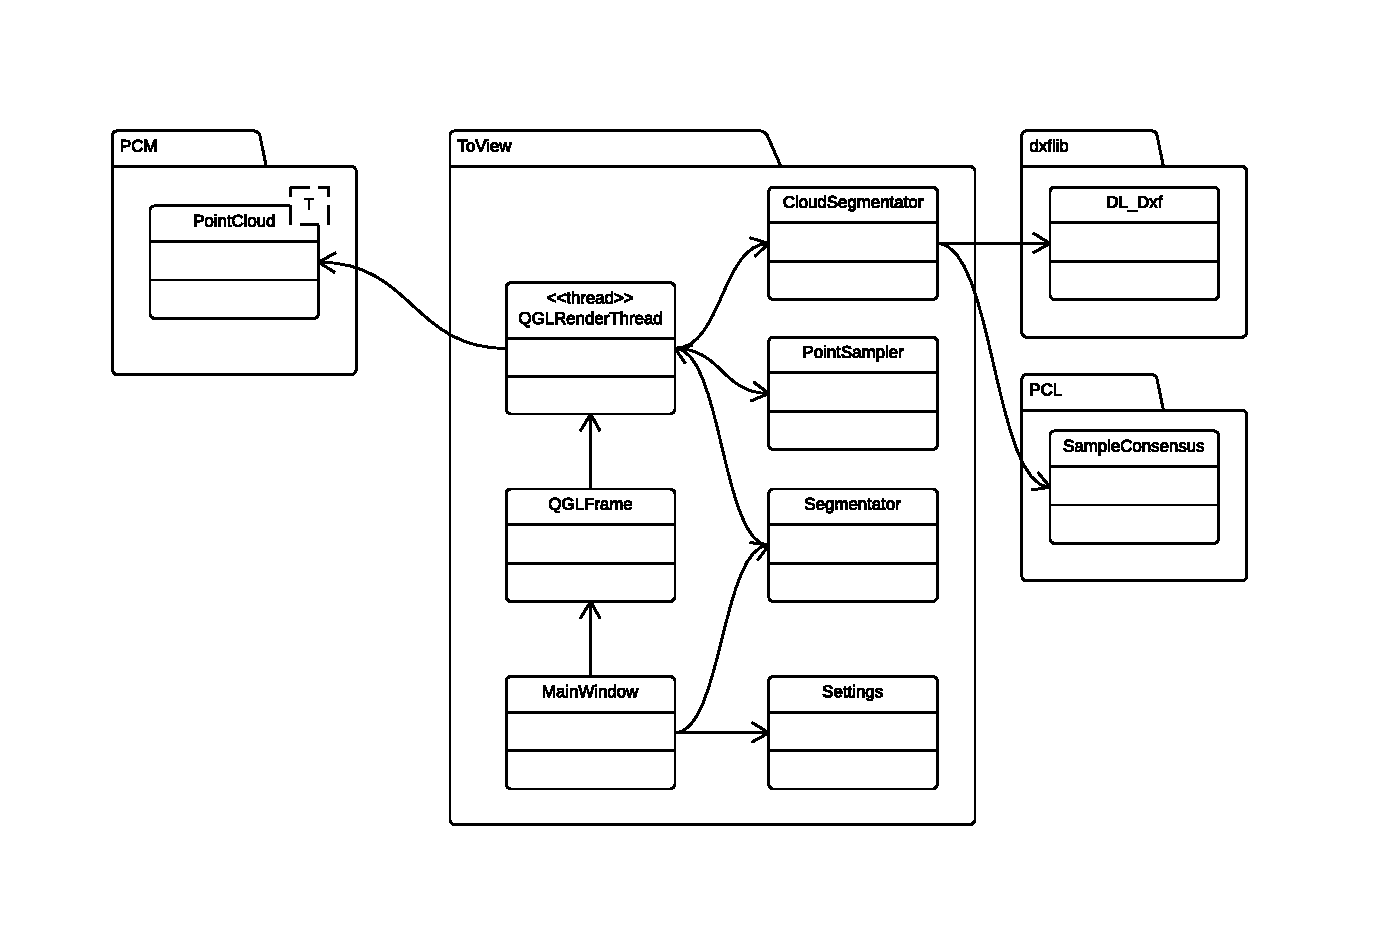
\includegraphics[scale=0.6]{figures/ToView.pdf}
                \caption[ToView class diagram]{
                        ToView class diagram.
                }
                \label{class_dia_tov}
\end{figure}

\textbf{PointCloud} represents a complete dataset and is the external interface of the library. It will allow the user to request information about the dataset, to load a region, apply a certain operation, etc. This class is accompanied by \textbf{PCMConfig} that stores several information about the characteristics of the point cloud.

On the other hand we have the visualizer \textbf{ToView} (see \figurename~\ref{class_dia_tov}) that is formed by:

\textbf{MainWindow} is the class that represents the main window of the visualizer. It contains the navigation menus and the widget in which the rendering will be done. The \textbf{Settings} class is where all the information related to the configuration of ToView will be stored and provides the interface to modify it. \textbf{Segmentator} is in charge of providing the interface for the user to be able to control and use the segmentation feature of the visualizer and modify its settings.

\textbf{QGLFrame} is responsible for creating the OpenGL context. It is also in charge of processing mouse and keyboard events. The rendering thread \textbf{QGLRenderThread} will also be launched from this class. As the name implies, this is the class that renders the point clouds. 

\textbf{PointSampler} will allow the user to sample points from a point cloud to be able to measure distances or segment primitives later. \textbf{CloudSegmentator} is the class responsible for segmenting and exporting the supported primitives.     





	%
% T�TULO DEL CAP�TULO
%
\chapter[PCM]{
	Point Cloud Manager
	\label{chapter_5}
}

\textbf{PCM} is a set of software tools and libraries that allow the user to manage massive point clouds. It comprises a new point cloud format, a multi-resolution spatial structure, a cache system and an external interface. 

\section[Design]{Design}

PCM is also developed following an object oriented approach and using the C{}\verb!++! language. The compilers used are the same as in the visualizer. The technologies chosen are also the same with an addition. For GPGPU programming we have chosen OpenCL, because of its inter-operation capabilities with OpenGL. This will allow us to process directly data that already resides in the GPU, without having to do expensive memory transfers. Because of the open nature of OpenCL, the software will be able to run on any graphics card vendor (AMD, NVIDIA or Intel) and the SO that the user prefers (Windows, MacOS or Linux).

\subsection[Dataset conversion and management]{Dataset conversion and management}
\label{subsec:conv}

\begin{figure}[h]
	\centering
	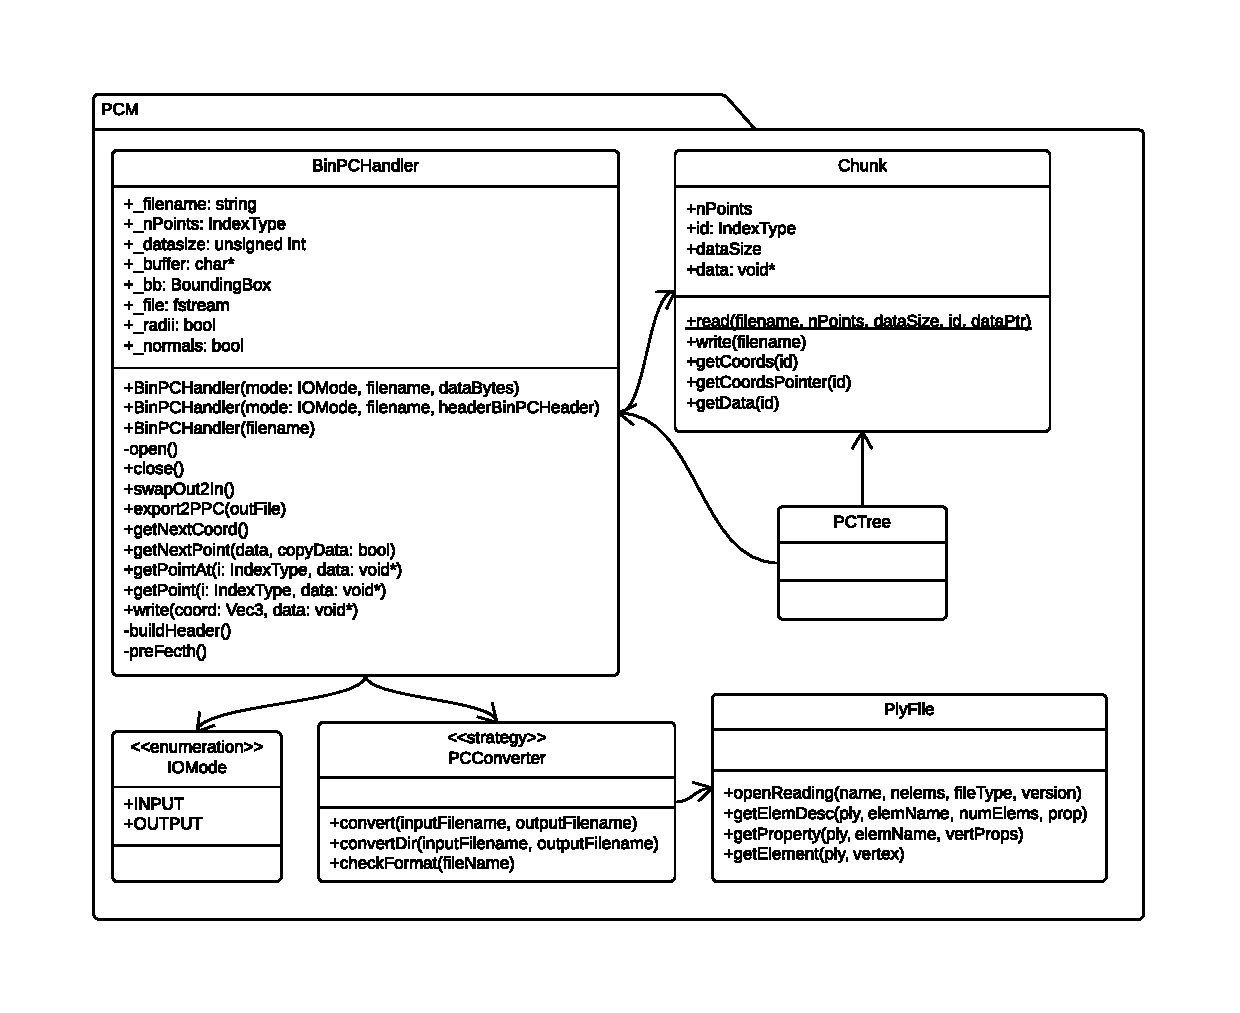
\includegraphics[scale=0.7]{figures/conv_man.pdf}
	\caption[Conversion and management of datasets class diagram]{
		Class diagram of the dataset conversion and management classes.
	}
	\label{conv_man}
\end{figure}

In the diagram in \autoref{conv_man}, the following classes are the most relevant:

\begin{itemize}
	\item \textbf{Chunk:} Minimum unit of data that will be managed by the different cache levels. Its size has to be strictly controlled because of this (no extra information just the basic information necessary to use it). Only has methods to read/write from/to disk.  
	\item \textbf{BinPCHandler:} This class represents the binary format used in the format conversion process and the spatial structure construction. Its objective is to emulate a STL vector, but that resides in disk instead of system memory. This is necessary because during the construction, operations like the calculation of the median will use the whole cloud that will not fit in RAM. With this class, the cloud can be used like if it would fit in primary memory. To improve the performance, it will \textit{pre-fetch} and \textit{buffer} data, after a certain number of requests. It will also allow writing and reading. This class has great performance when accessing data sequentially, but it is not as efficient for random access. 
	\item \textbf{PCConverter:} This will be the class that will provide a single interface to convert any type of point cloud to BPC. The ``strategy'' pattern was used to create this class. It first checks the format of the input point cloud and then delegates the responsibility to the adequate method. It can convert a single file or a set of files stored in a folder.
\end{itemize}

\subsection[Spatial data structure]{Spatial data structure}

The most important class in \autoref{tree_class} is \textbf{PCTree}. The class will encapsulate two of the main functionalities:

\begin{figure}[h]
	\centering
	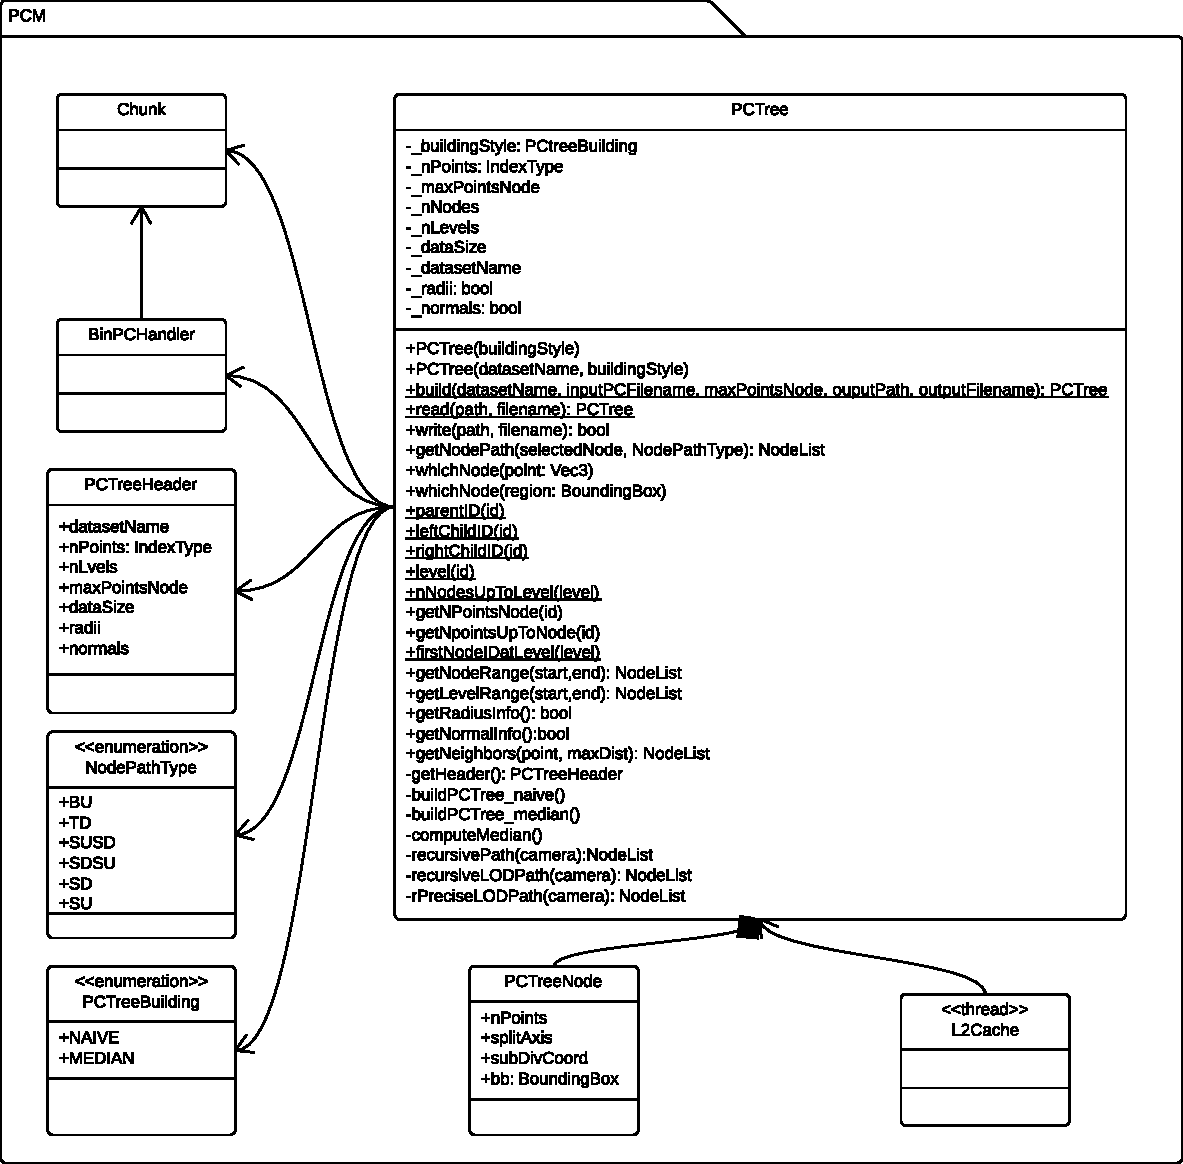
\includegraphics[scale=0.6]{figures/tree_class.pdf}
	\caption[Data strucuture class diagram]{
		Class diagram of the spatial data structure.
	}
	\label{tree_class}
\end{figure}

\begin{itemize}
	\item The construction of the chunk DB and the spatial structure itself. This is done as a pre-process, before using the library. This can be achieved using \textit{PCGen}\footnote{A provided command line utility.} or using the visualizer. 
	\item Managing the multi-resolution tree, obtaining \textit{NodePaths}\footnote{List of nodes to reach a certain area from the tree root.} and performing tree traversals.
\end{itemize}

The tree nodes, represented by the class \textbf{PCTreeNode}, are all kept in a lineal vector for quick access ($O(1)$). There are also some functions valid for any binary tree related to the traversal of the tree; getting the child nodes of a parent, level of a node, etc. There are also functions to read/write the tree from/to disk. Finally, there are also functions to build priority node lists for the visualizer.

TODO assembler log?   

\subsection[Memory hierarchy]{Memory hierarchy}

\begin{figure}[h]
	\centering
	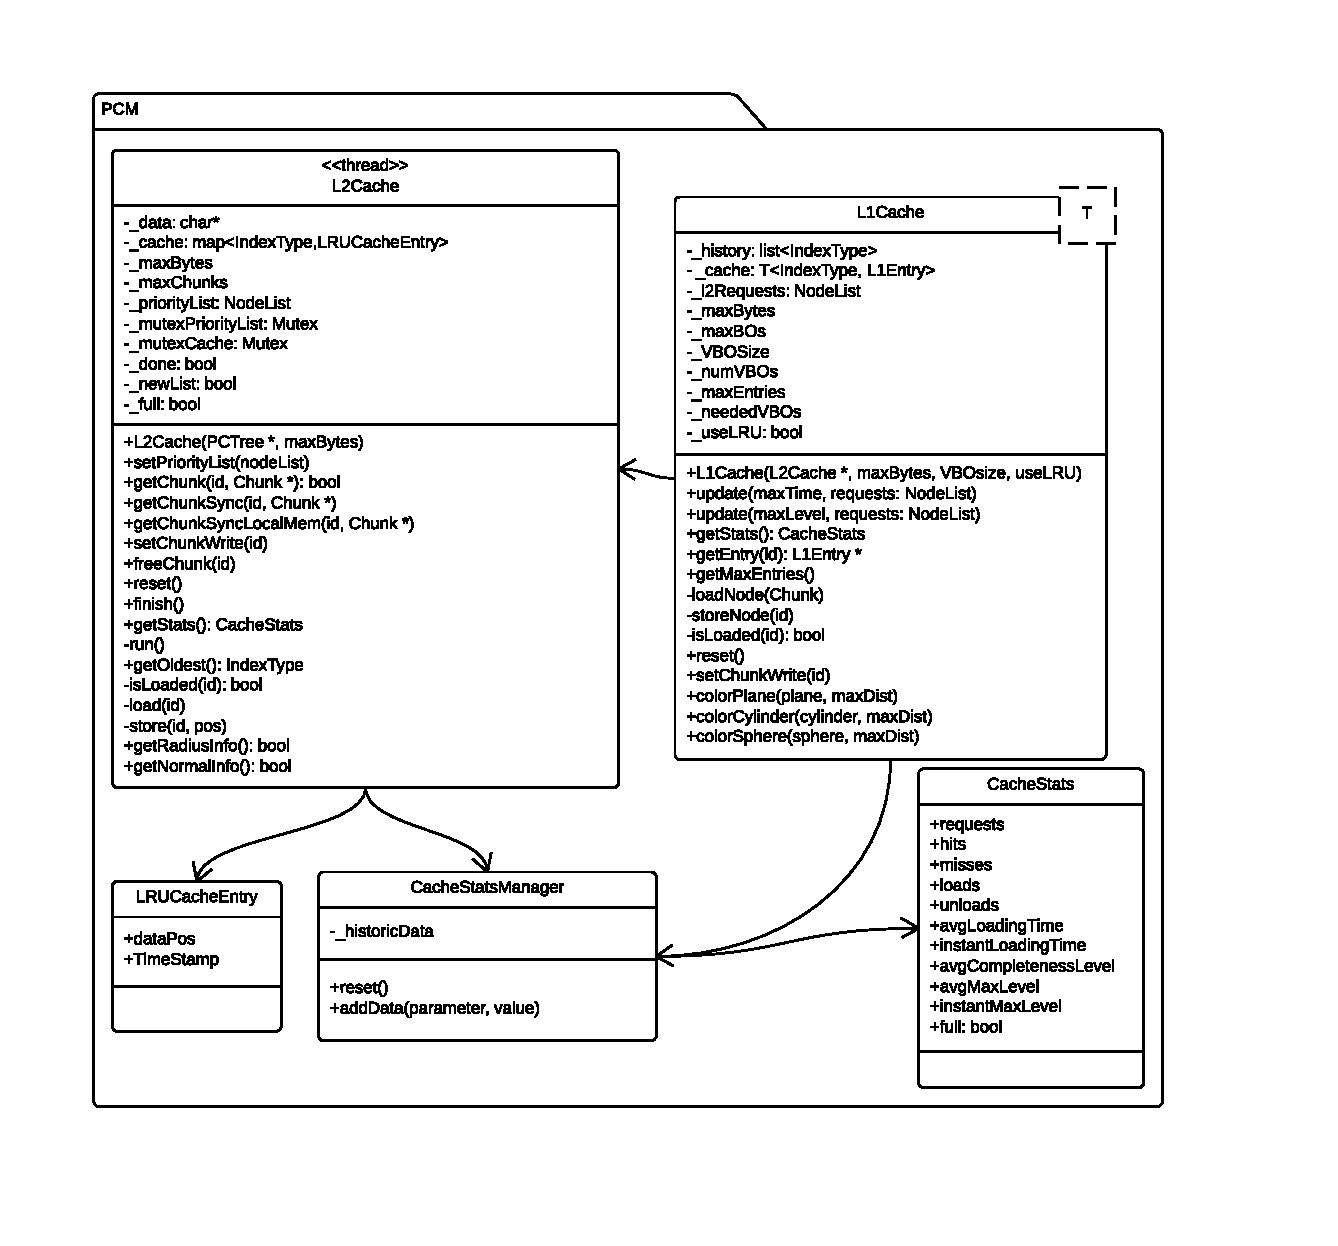
\includegraphics[scale=0.6]{figures/hier_class.pdf}
	\caption[Memory hierarchy class diagram]{
		Class diagram of the memory hierarchy.
	}
	\label{hier_class}
\end{figure}

In \autoref{hier_class} the most significant classes are:

\begin{itemize}
	\item \textbf{L1Cache:} Responsible for loading/storing data in VRAM/RAM and the conversion of chunks in one or multiple VBOs. The class uses a variadic template to let the user choose the type of cache container (\textit{\_cache}). The \textit{update()} method will take care of making the requests to the L2 and the VBO conversion using \textit{load() and store()}.   
	\item \textbf{L2Cache:} Is the class responsible for loading/storing data in RAM/HDD, it inherits from \textbf{Thread} so that it runs on its own thread. As we will mention in \autoref{subsec:L2}, a Map (\textit{\_cache}) keeps references to every chunk that is loaded in the \textit{\_data} attribute. The request list is kept in the attribute \textit{\_priorityList}. Both structures are protected by \textit{Mutex} and a custom \textit{Semaphore}. The \textit{run()} method contains the main loop. 
	\item \textbf{CacheStatsManager:} Both of the previous classes contain an instance of this class. It is in charge of the monitorization of the caches, to get statistics of the cache status. Hits, misses, forced misses, load times, etc.  
\end{itemize}

\subsection[External interface]{External interface}

\begin{figure}[h]
	\centering
	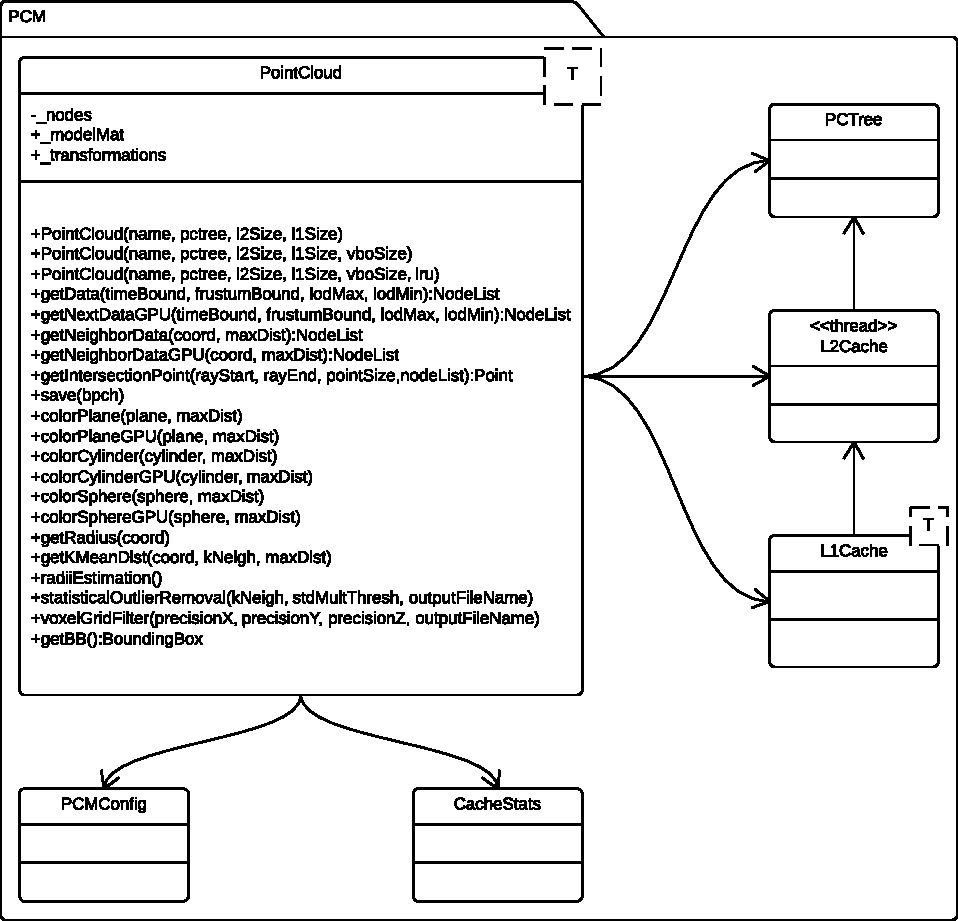
\includegraphics[scale=0.6]{figures/external_interf.pdf}
	\caption[External interface class diagram]{
		Class diagram of the external interface.
	}
	\label{external_interf}
\end{figure}

In \autoref{external_interf} the most important class is \textbf{PointCloud}, this class represents a complete dataset. This class will allow to load or save a dataset, request information about it, request to load an area or access to the spatial structure so that the user can make queries. 

This class is used extensively by the visualizer to simplify the render process. It also provides several point cloud operations, like an statistical outlier removal filter, a voxel filter, radii estimation, etc.

\section[I/O]{Input and output}

This project will support a certain number of common point cloud data input formats. Furthermore, it can also output point cloud or geometric data in certain formats. In this section we will explain all the details related to these two subjects.   

\subsection[Supported point cloud formats]{Supported point cloud formats}

Several new point formats have been added to the capabilities of the point cloud converter utility. PCM will identify automatically the point cloud format and convert it to our own format transparently for the user. 

The supported point cloud input formats are:

\begin{itemize}
	\item \textbf{PTS:} Common ASCII point data format. The first line has the number of points to read, and the rest of the lines all the point data: $(x,y,z) + reflectivity + (R,G,B)$.
	\item \textbf{PTX:} ASCII laser scanning format. The first lines have information about the scan and the number of points scanned. The rest of the lines contain all the point data: $(x,y,z) + reflectivity + (R,G,B)$. 
	\item \textbf{ASC:} Common ASCII point data format in which every line contains information about each point in the cloud: $(x,y,z) + reflectivity + (R,G,B)$.
	\item \textbf{LAS:} Binary laser scanning format, it contains all sorts of information about the scan and the point data that can include: $(x,y,z) + reflectivity + (R,G,B)$.
	\item \textbf{PLY:} PLY is a computer file format known as the Polygon File Format or the Stanford Triangle Format. It can be binary or ASCII, and the project supports both. It contains the following information: $(x,y,z) + (R,G,B) + (n_{x},n_{y},n_{z})$.
	\item \textbf{PCD:} The point cloud format of one of the most used point cloud libraries, \textbf{PCL} \cite{PCL}. As the preceding format, it can be binary or ASCII. Each point can have: $(x,y,z) + (R,G,B)$.   
	\item \textbf{BPC:} Our own binary point cloud data format. It stores information about the cloud and individual points. Each point can have: $(x,y,z) + (R,G,B) + radius + (n_{x},n_{y},n_{z}) + etc$.
\end{itemize}  

Because of the size that this files can reach, they normally are split in several smaller files that range from 500 MB to 1,5 GB. Because of this reason, the ability to read multiple point cloud files in a folder automatically will also be added. 

\subsection[BPC]{Binary Point Cloud}

The point cloud format created for this project (BPC) will now be detailed. It is a binary format that is comprised of a \textbf{header} and the \textbf{point cloud data}. 

The header will contain the following information:

\begin{itemize}
	\item \textbf{Number of points:} The number of points contained in the file.
	\item \textbf{Data size:} Size of the data that accompanies the point (normals, radii, etc.). 
	\item \textbf{Bounding box:} Information of the bounding box that contains the point cloud.
	\item \textbf{Radii:} Indicates if the dataset contains point radii.
	\item \textbf{Normals:} Specifies if the point normals are available.
\end{itemize}  

The rest of the file will contain the point cloud data. The data will be stored contiguously point after point as can be seen in \autoref{chunk} to minimize the file size.

\begin{figure}[h]
	\centering
	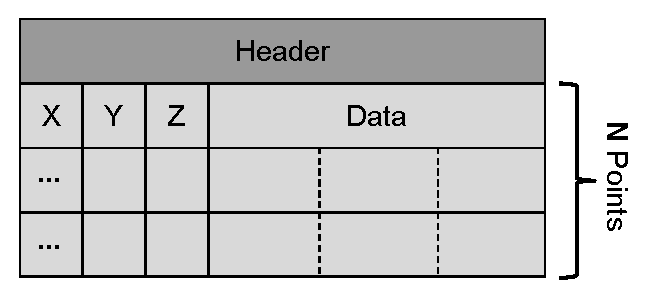
\includegraphics[scale=0.8]{figures/chunk.pdf}
	\caption[Chunk structure]{
		Chunk structure.
	}
	\label{chunk}
\end{figure}

A BPC file is treated like a single chunk that contains the whole cloud, so all of this information is also valid for chunks. A chunk will be the minimum amount of information that the memory hierarchy will deal with. When rendering, the whole cloud will not be stored in a single chunk, since this would not be efficient. Instead, the points in the nodes of the multi-resolution structure will each be stored in a chunk, and the cloud will be an aggregate of all the chunks (see \autoref{chunk_tree}). 

\begin{figure}[h]
	\centering
	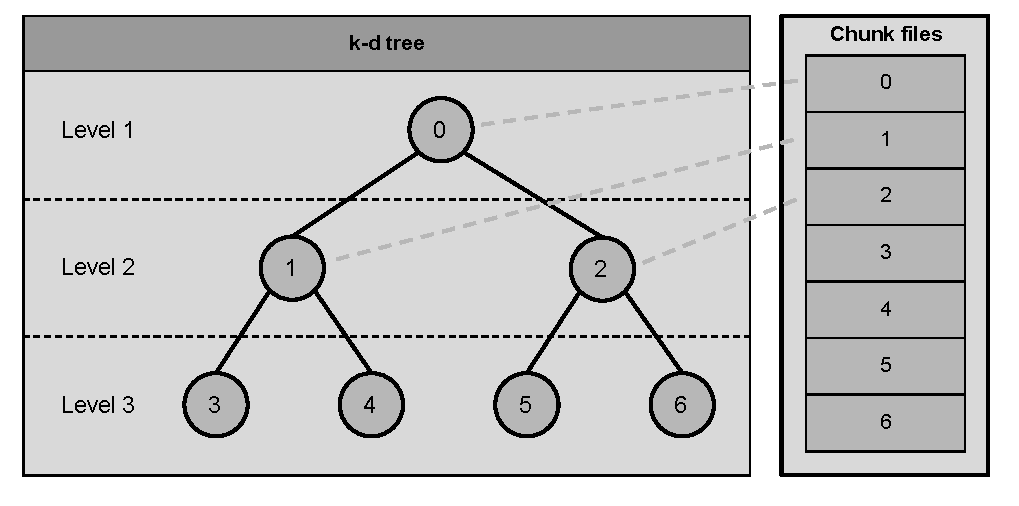
\includegraphics[scale=0.8]{figures/chunk_tree.pdf}
	\caption[Internal tree structure]{
		Internal tree structure. Each node is stored in a chunk file.
	}
	\label{chunk_tree}
\end{figure}

The only big difference between a BPC file and a chunk, is that because the size of a BPC file will be much greater. Therefore it will not be possible to load the complete file at once, and we will rely on an interface class, \textbf{\textcolor{Emerald}{BinPCHandler}}. This interface works in a similar manner to an array in system memory, but accessing permanent memory in an efficient way (this class will be further explained in the \autoref{subsec:conv}). 

\subsection[Output]{Output}

\section[Memory hierarchy]{Memory hierarchy}

One of the principal concepts in PCM is the memory hierarchy management, that is made up of two levels of cache. When it is known that the data that is going to be used is related in some way and the different access types, software caches can yield substantial improvements in the performance of the system. In this case, we work mainly with geometric information obtained from real environments and the cache hierarchy will allow us to exploit the spatial coherence in the data.  

In this project, a cache system with two levels has been implemented. It will take care of the data transfer needs between memory levels (HDD - RAM - VRAM). This system will take into account the spatial relation between the data, and will have an architecture that will not only allow to store datasets in a HDD but anything with a filesystem (e.g. NFS from a network).

\begin{figure}[h]
	\centering
	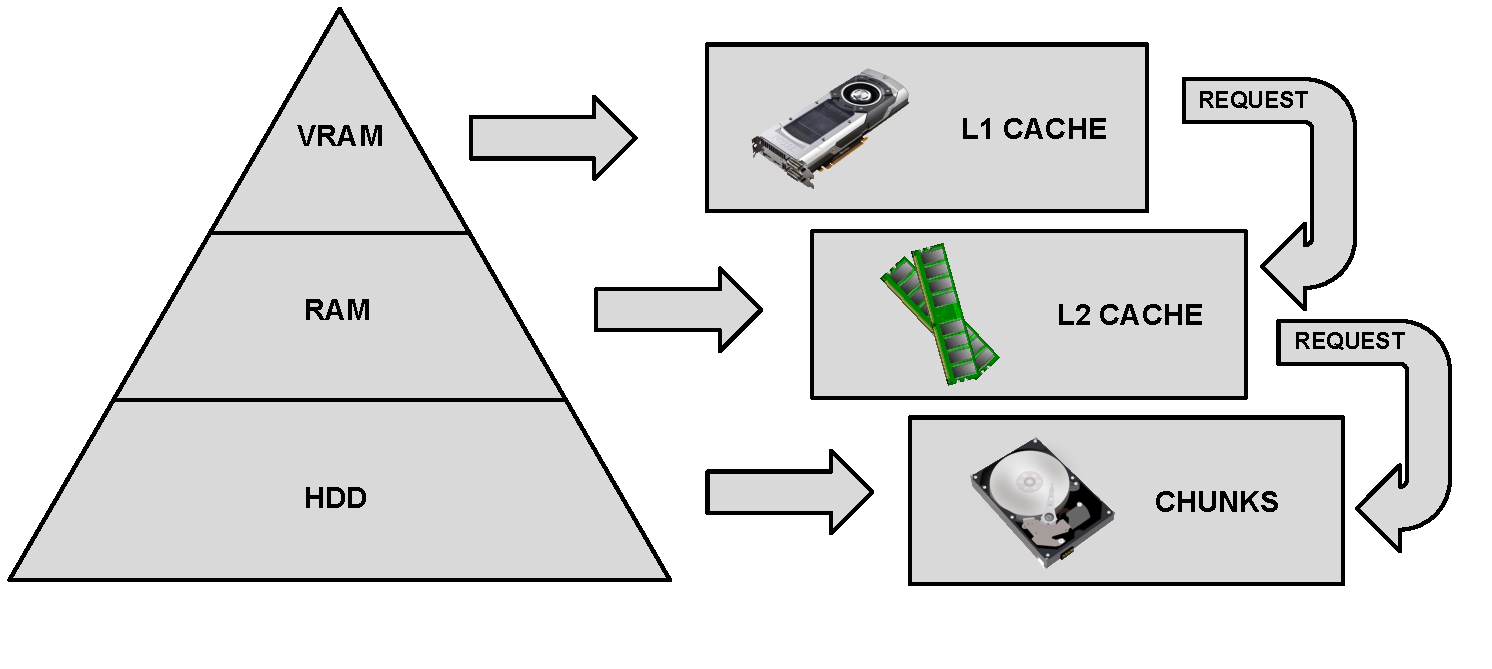
\includegraphics[scale=0.5]{figures/mem_hierch.pdf}
	\caption[Memory hierarchy]{
		Memory hierarchy of PCM.
	}
	\label{mem_hier}
\end{figure}

Between these three levels of memory will circulate the minimum unit of information, the chunk. A chunk is a ``container'' of a data subset, in our case points and data related to them.

The three levels are:

\begin{itemize}
	\item \textbf{Video memory or VRAM:} Volatile memory and less capacity than the next level, but even faster. Only the GPU will use this type of memory. The L1 cache will be created in this memory level.
	\item \textbf{Primary memory or RAM:} Volatile memory and low capacity compared to the next level, but fast. The CPU will use this type of memory. The L2 cache will reside in this cache level. 
	\item \textbf{Secondary memory or HDD:} Persistent memory and high density, but slower than the other two levels. In this level of memory will reside the point database.  
\end{itemize}  

First, in the lowest level, reside the binary files of each chunk. In the next level, RAM memory, a subset of chunks will be stored. Finally in VRAM, the chunks are adapted to a video memory compatible format, so that the GPU can work with them. 

These concepts will be further explained in the next subsections. 

\subsection[L1]{L1 cache}

The first level cache (L1) is in charge of managing the storing and loading of data between primary memory (RAM) and video memory (VRAM). This cache level has been completely reworked, and also has been given the ability to not only load but also store information in primary memory. Even having a similar structure to the L2 cache, because of the characteristics of GPU processes, its operation is synchronous. 

Its biggest responsibility, apart from the corresponding memory hierarchy management, will be the conversion of chunks of data to \textit{VBOs}\footnote{\textit{Vertex Buffer Object}: Structure that allows to store arrays of data in video memory.} in VRAM and viceversa. A chunk may have to be broken up into several VBOs depending on its size, so that optimal sizes of VBOs can be maintained for the GPU.

\begin{figure}[h]
	\centering
	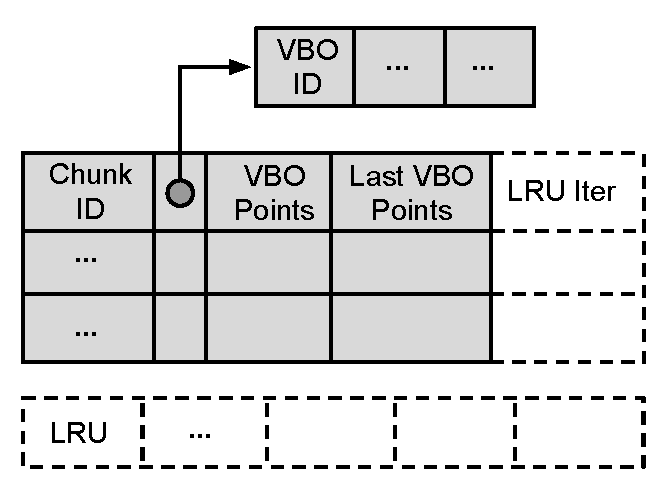
\includegraphics[scale=0.7]{figures/l1_cache.pdf}
	\caption[L1 cache structure]{
		L1 cache structure.
	}
	\label{l1_cache}
\end{figure}

The following list will explain each of the fields that make up the cache structure (see \autoref{l1_cache}):

\begin{itemize}
	\item \textbf{Chunk ID:} Id of the chunk stored in L1 cache.
	\item \textbf{VBO ID:} IDs of the VBOs used to store points in the L1 cache entry.
	\item \textbf{VBO Points:} Number of points stored in all but the last VBO in the cache entry.
	\item \textbf{Last VBO Points:} Number of points in the last VBO in the cache entry.
	\item \textbf{LRU Iter:} Iterator to cache entry in LRU access record for fast updating of LRU.
	\item \textbf{LRU:} Least Recently Used chunk. 
	\item \textbf{Write:} Flag that marks chunk for storing. 
\end{itemize} 

Also two replacement policies were implemented:

\begin{itemize}
	\item \textbf{Naive:} Erase any data block that is not necessary looping over the complete cache one time. This method does not take into account when was the last time that a block was last used, if it is not necessary it will be erased. 
	\item \textbf{LRU\footnote{\textit{Least Recently Used}}:} This algorithm, will replace the elements that have been used least recently if the cache is full. If not full it will keep inserting nodes until it is.  
\end{itemize} 

To store the list of nodes currently in the cache two STL\footnote{\textit{Standard Template Library}} data structures can be used:

\begin{itemize}
	\item \textbf{Map:} An associative container with key-value pairs with ordered unique keys. Complexity of searches and element access is logarithmic in size: $O(\log n)$. 
	\item \textbf{HashMap:} It also contains key-value pairs with unique keys but without an order, element access is done using a hash function. Complexity of searches and element access is constant in the average case: $O(1)$ and linear in size in the worst case: $O(n)$.
\end{itemize}

Either of these two structures will meet our objective of making cache searches fast, as this is a crucial function that will be frequently used. Theoretically the use of one or the other depends on the number of nodes that the cache will contain. A Map will be faster with less elements, while the HashMap will be faster with big quantities of nodes. 

Another implemented feature are types of cache requests, there are several available:

\begin{itemize}
	\item \textbf{Restricted by time:} In order for the render process to be interactive and that no freezes occur, we will limit loading of VBOs by time. This type of petition will be limited by the time that the user desires (e.g. 3 ms). The cache will load as much nodes as possible in the given time and if the maximum time is reached it will stop loading nodes, even if there are still nodes missing. 
	\item \textbf{Restricted by level:} This type of request is usually used in GPGPU calculations, where no interactivity is needed. The user will specify a level of precision and the cache will load as many nodes as necessary for that level of detail.
\end{itemize}

This cache not only can read and load nodes from L2, it also has the ability to store changes made in video memory (L1) in RAM (L2). The user can choose if he wants the changes made in GPU (e.g. an OpenCL kernel) to be persistent or not.

When the node is evicted from the cache, its changes will be written to the L2 cache prior to its deletion. In the \autoref{l1_write} we not only show how to write changes to other cache levels, but also how to use PCM with its new \textbf{\textcolor{Emerald}{PointCloud}} interface to loop over the complete cloud out of core and perform some custom operation.

This process is completely transparent for the user, that will only have to use this example code:
\\
\lstset{language=C++,frame=shadowbox,rulesepcolor=\color[gray]{0.8},lineskip=10pt, 
		keywordstyle=\color{VioletRed}\bfseries,
		emph={PointCloud}, emphstyle=\color{Emerald}\bfseries,
		emph={[2]setChunkWriteL1,getNextDataGPU,getL1Entry,makeChangesGPU}, emphstyle={[2]\color{PineGreen}},label={l1_write} }
\begin{lstlisting}
 PointCloud cloud(...);

 while (cloud.getNextDataGPU(list)) {
 	for (auto& node:list) {		
		auto * VBOdata = cloud.getL1Entry(node);
		if (VBOdata) {
			makeChangesGPU(node);
			cloud.setChunkWriteL1(node);
		}		
	}
 }
\end{lstlisting}

\subsection[L2]{L2 cache}
\label{subsec:L2}

The second level cache L2, will be in charge of transferring data (chunks) from disk to system memory (RAM). The replacement policy used in this cache is LRU \cite{taibo} as this is the most adequate policy for these types of systems. 

To better use the resources available nowadays (multi-core CPUs), this cache will run on its own thread. Also since the massive datasets that we will deal with require a lot of computational power for even the simplest operations, this cache will be prepared to deal with simultaneous requests from different work threads. All of this is achieved with careful use of \textit{mutex}\footnote{A synchronization mechanism for enforcing limits on access to a resource in an environment where there are many threads of execution.} and \textit{semaphores}\footnote{A variable or abstract data type that is used for controlling access, by multiple processes, to a common resource in a parallel programming or a multi user environment.}. 

\begin{figure}[h]
	\centering
	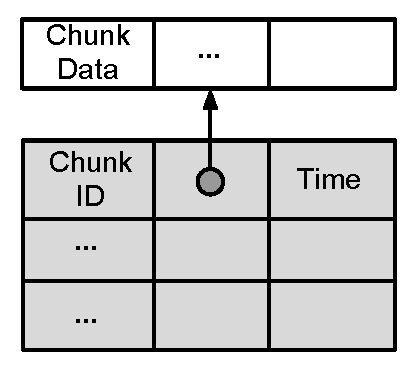
\includegraphics[scale=0.9]{figures/L2.pdf}
	\caption[L2 structure]{
		L2 cache structure.
	}
	\label{l2_structure}
\end{figure}

The following list will explain each of the cache structure fields (see \autoref{l2_structure}):

\begin{itemize}
	\item \textbf{Chunk ID:} Id of the chunk stored in L2 cache.
	\item \textbf{Position:} Position of the chunk in the structure that contains all of them.
	\item \textbf{Time:} Time in which the node was last accessed.
\end{itemize} 

Next, the responsibilities of the L2 cache are:

\begin{itemize}
	\item Load petition lists from disk that are requested by the upper cache level (L1).
	\item Keep a ``repository'' of recently loaded chunks, that because of the nature of the spatial structure, will be utilized again with a high probability. 
	\item Ask the spatial structure which files correspond to the requested nodes.
	\item Keep memory coherence of the system, with a Map that matches node IDs with their corresponding chunk in memory. 
	\item If the user desires it, write changes to disk.   
\end{itemize} 

The main loop can be summed up in the following actions. First, it waits until a new petition arrives, when it does, it loads the requested nodes in order. If during the loading of the list a new one appears, the old one is discarded and the process begins again.

This cache can work in one of two ways:

\begin{itemize}
	\item \textbf{Synchronous:} A node is requested and loaded immediately. 
	\item \textbf{Asynchronous:} A list of nodes is requested and they are loaded in order as soon as possible.
\end{itemize}

This cache is capable of not only reading data from the HDD, but also writing modified data from RAM to disk. This is achieved in a similar fashion to the L1. A complete loop over the whole cloud to perform an operation using the CPU and then writing it to disk, can be seen in \autoref{l2_write}.
\\
\lstset{emph={PointCloud,Chunk}, emphstyle=\color{Emerald}\bfseries,
		emph={[2]setChunkWriteL2,getNextData,getChunkL2,makeChanges,freeChunkL2}, emphstyle={[2]\color{PineGreen}},label={l2_write}}
\begin{lstlisting}
 PointCloud cloud(...);

 while (cloud.getNextData(list)) {
 	for (auto& node:list) {		
		Chunk chunk;
		cloud.getChunkL2(node, chunk);
		makeChanges(chunk);
		cloud.setChunkWriteL2(node);	
		cloud.freeChunkL2(node);	
	}
 }
\end{lstlisting}

The cache hit rate will be really high, because of the topology of the spatial structure. If an algorithm needs to reach the maximum level of detail in different zones, because the levels are additive, it will have to add up all the information contained in the node path from the root to the leaf. But in regions of space that are close, that means they will share a lot of nodes (see \autoref{node_sharing}). 

\begin{figure}[h]
	\centering
	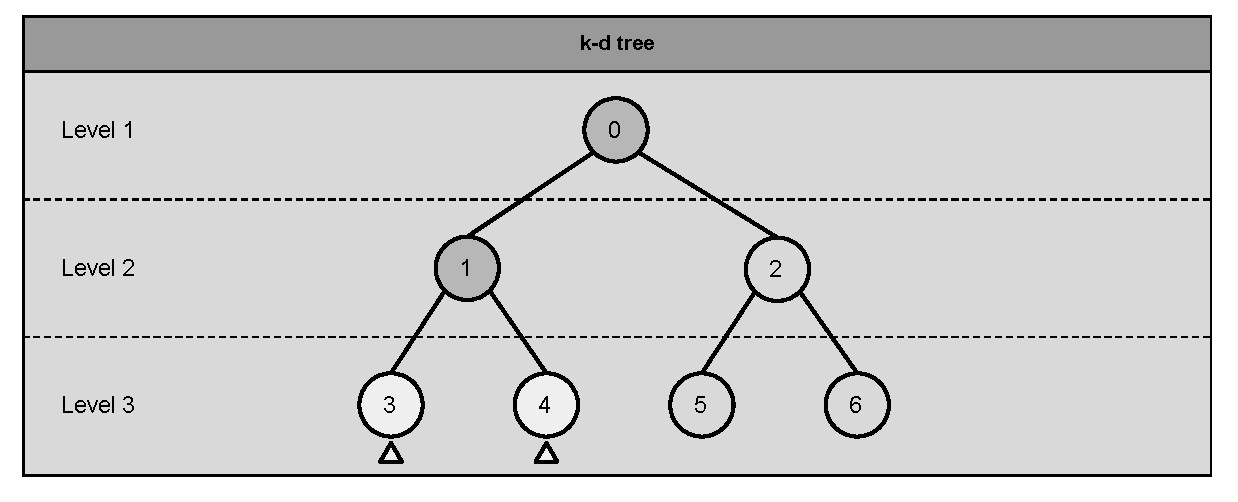
\includegraphics[scale=0.6]{figures/node_sharing.pdf}
	\caption[Common nodes close paths]{
		Two node paths spatially close (3 and 4), in order to reach the maximum level of detail (level 2) share nodes 0 and 1.
	}
	\label{node_sharing}
\end{figure}

\subsection[PCM Benchmark]{PCM Benchmark}

Since we wanted to have a quick and convenient way to test PCM, we created this utility in \textit{Python} to achieve this purpose. PCMBenchmark is a Python benchmark suite that automatically tests PCM and outputs the corresponding metrics for the user to see or use. 

In order for PCMBenchmark to work it uses a certain directory structure:

\begin{itemize}
	\item \textbf{bin:} With \textbf{debug} and \textbf{release} sub-directories that contain the corresponding PCM executables (user creation required).
	\item \textbf{dataset:} Contains the test dataset (user creation required).
	\item \textbf{data:} Automatically created directory that contains testing data. This is raw data just in case the user will want to process the data on its own.
	\item \textbf{trees:} Automatically created directory that contains automatically generated k-d trees.
\end{itemize} 

\begin{figure}[h]
	\centering
	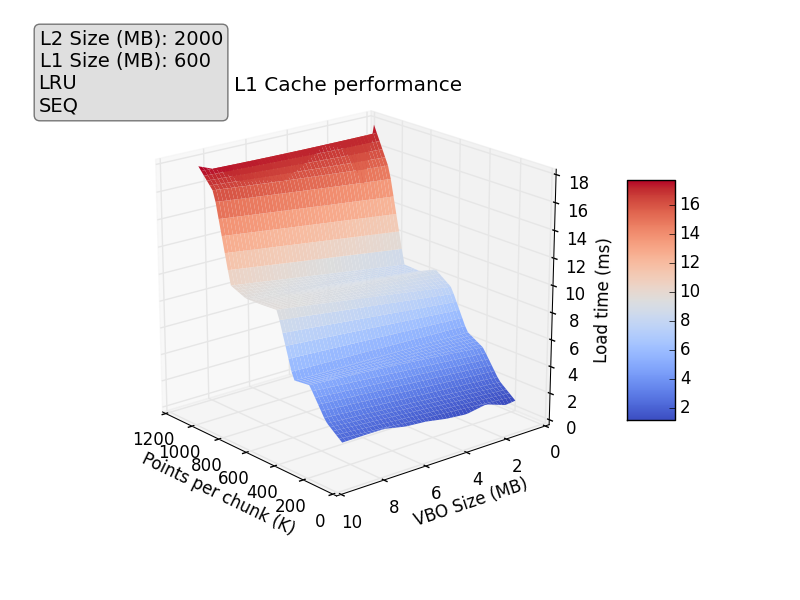
\includegraphics[scale=0.7]{figures/benchmark.png}
	\caption[Sample PCMBenchmark output]{
		A sample output graph created by the benchmark suite.
	}
	\label{benchmark}
\end{figure}

Once the user has the directory structure created, its just a matter of copying and pasting to test PCM in different machines. The process will be completely transparent for the user that will only need to check the resulting graphs (see \autoref{benchmark}).

The outputs that the benchmark suite creates are:

\begin{itemize}
	\item \textbf{Graphs:} Available in the root directory as a series of .png files. This is the most user friendly output of the tool, a series of graphs that show the metrics in a graphical sense.
	\item \textbf{System information:} Stored in a text file called \textit{sys\_info.txt} that contains common system info.
	\item \textbf{Raw data:} Automatically generated data to create the graphs. Suitable for further processing by an advanced user.
\end{itemize} 

The only system requirements are:

\begin{itemize}
	\item \textbf{Python 3.3}
	\item \textbf{MatPlotLib}
	\item \textbf{NumPy}
\end{itemize} 

With this tool the testing in multi-platform environments is greatly simplified.

	%
% T�TULO DEL CAP�TULO
%
\chapter[ToView]{
	ToView
	\label{chapter_6}
}

ToView is how we named the visualizer that uses PCM under the hood, it was also implemented using C{}\verb!++!, OpenGL for visualization purposes and QT \cite{QT} for the user interface. All of these choices will be explained in the rest of the chapter.

\section[Design]{Design}

The visualizer has been implemented using \textbf{OpenGL 4.3} and \textbf{QT 5.3}. These two technologies were chosen so that the compatibility with multiple platforms was kept. Either OpenGL or QT are compatible with Windows, Linux and MacOS X.

On one hand, OpenGL is an API that allows an application to access and control the graphical system of the machine in which it is being executed. It could be a workstation with a high performance graphics card or a common desktop computer, a video-games console, etc.  

On the other hand, QT is a multi-platform graphical application creation framework. QT is open-source software that has been used and improved since it was created. It fits perfectly with our project since is C{}\verb!++! based. 

QT is used in more than 70 industries, by leading companies in their markets. QT is intuitive, has a suite for the design of interfaces called \textit{QT Designer} and plugins for the major development IDEs like Visual Studio.   

The compilers used as mentioned before are: Visual C{}\verb!++! in Windows systems, GCC in Linux and Clang in MacOS X.

\subsection[GUI]{Graphical User Interface}

\begin{figure}[h]
	\centering
	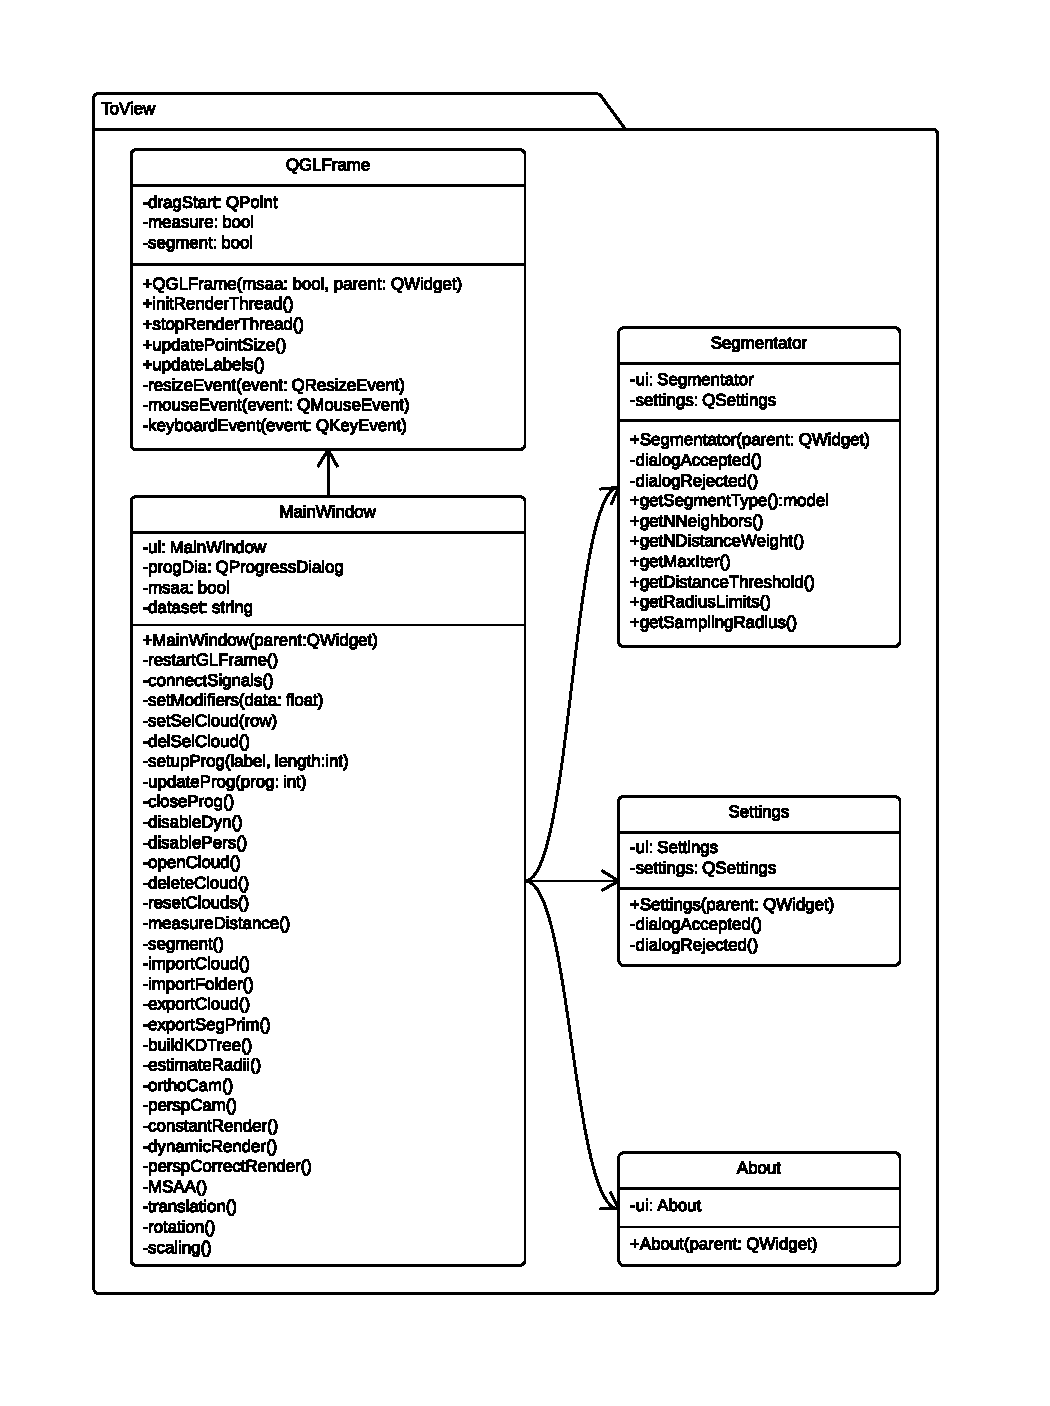
\includegraphics[scale=0.6]{figures/GUI.pdf}
	\caption[User interface class diagram]{
		Class diagram of the user interface of ToView.
	}
	\label{GUI}
\end{figure}

In the \autoref{GUI}, one of the main classes is \textbf{MainWindow}. This class gives the user access to all the functionality of the visualizer, it will serve as the name implies, as the main window in the interface. This class will centralize all the functionality and access to secondary dialogs, as well as communicate with the OpenGL context and render thread. 

The OpenGL context is represented in the interface by the class \textbf{QGLFrame}, that is in charge of creating the corresponding OpenGL context, render thread and displaying each frame rendered. This class will also handle all the keyboard and mouse events.  

The \textbf{Segmentator} class, is a sub-dialog that will let the user input the parameters for the segmentation of primitives in the clouds. All of the choices are saved using the \textbf{Qsettings} class. This QT class simplifies the process of managing settings in an application, eliminating the need for custom configuration files. 

Furthermore, \textbf{Settings} is another sub-dialog that allows the user to configure several visualizer parameters. This dialog also relies on \textbf{QSettings} to store the settings permanently. 

Finally, \textbf{About} is just another sub-dialog that shows information about the software (version, authors, etc.). 

\subsection[Render thread]{Render thread}

\begin{figure}[h]
	\centering
	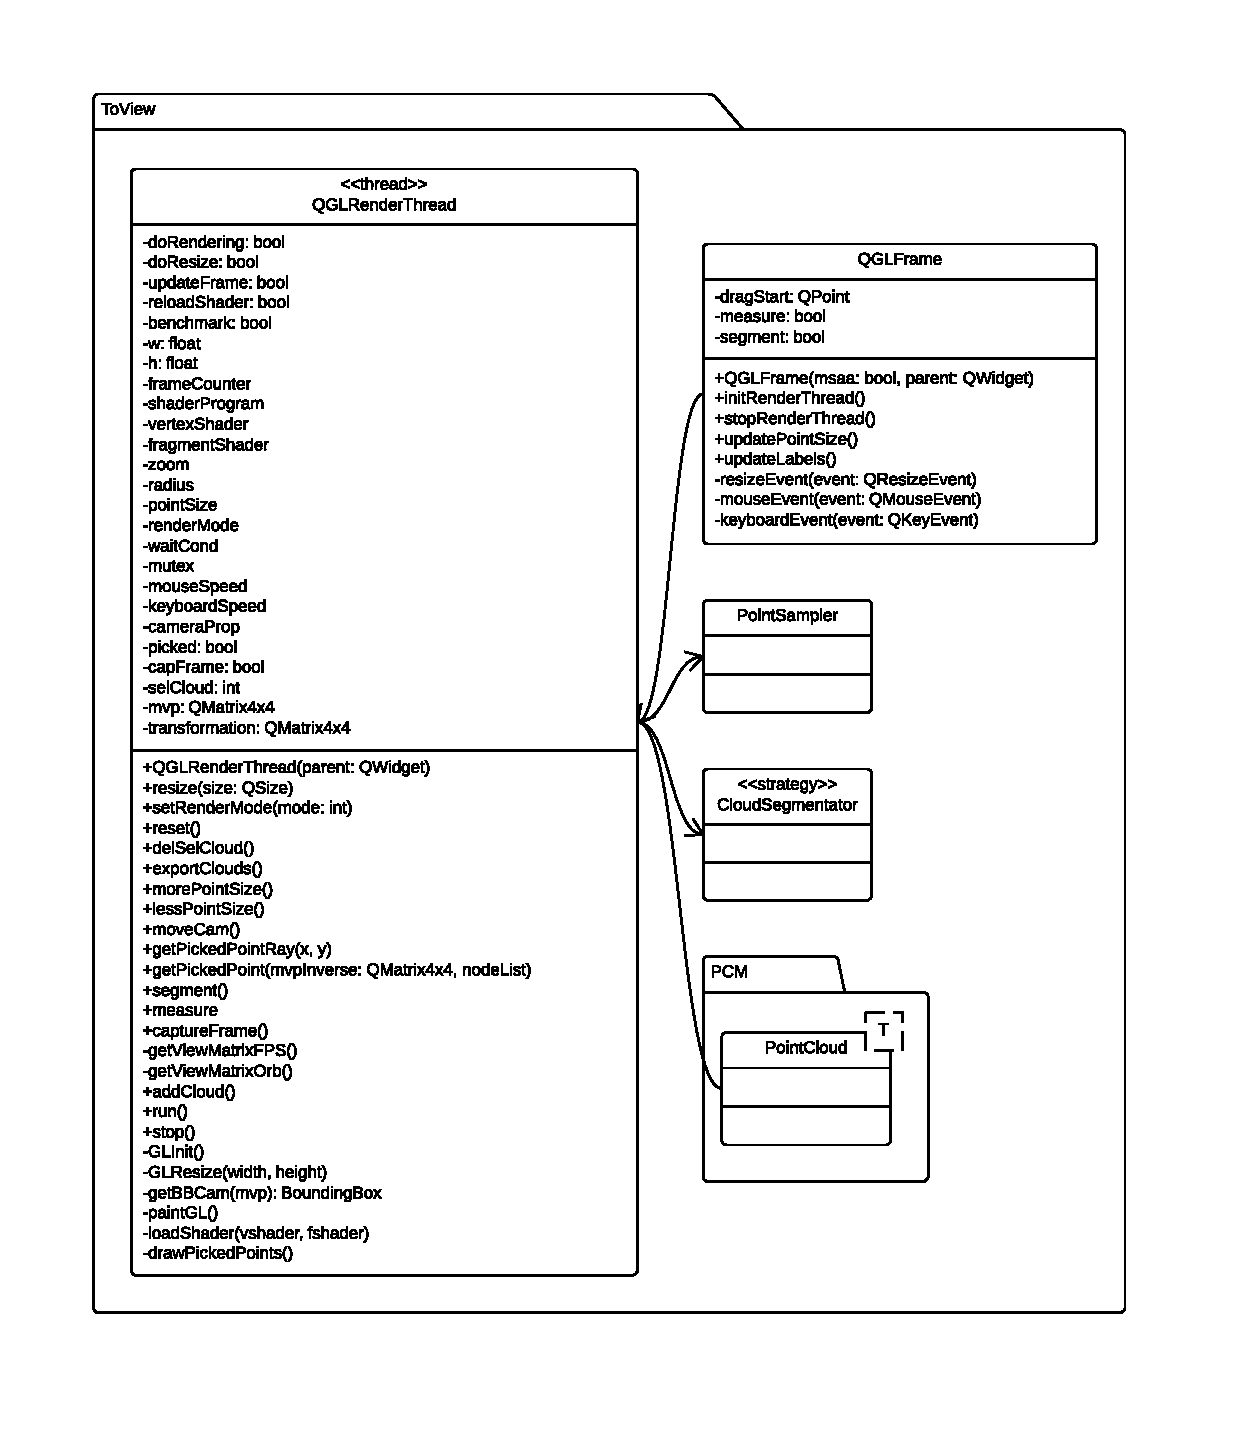
\includegraphics[scale=0.6]{figures/render_thread.pdf}
	\caption[Render thread class diagram]{
		Class diagram of the render thread and its related classes.
	}
	\label{render_thread}
\end{figure}

As we can observe in \autoref{render_thread}, \textbf{QGLRenderThread} is a extremely complex class, that as its name hints, represents a render thread. This class will be in charge of initializing OpenGL, loading shaders, rendering, calculating the camera parameters, etc.

The thread is created by \textbf{QGLFrame}, next the OpenGL context will be transferred to that thread so that the rendering can begin. Rendering is done in a different thread than the GUI, so that the latter will still be responsive even in the most demanding cases. 

Because of this, the communication between the render thread and the GUI will make use of QT \textit{signals} and \textit{slots}\footnote{Language tool introduced in QT for communication between objects, which allows the implementation of the Observer pattern. The concept is that GUI widgets can send signals containing event information, which can be received by other objects using special functions known as slots.}. With these tools, the communication between the different threads will be robust and simpler. Since the render thread could also be used from multiple threads, we will also use a \textit{mutex} to secure concurrent accesses.

To access the cloud information in PCM, the external interface \textbf{PointCloud} is used. \textbf{PointCloud} will provide the necessary information to render the desired clouds; like node lists, point data, memory hierarchy management, etc.      

\subsection[Segmentation]{Segmentation}

\begin{figure}[h]
	\centering
	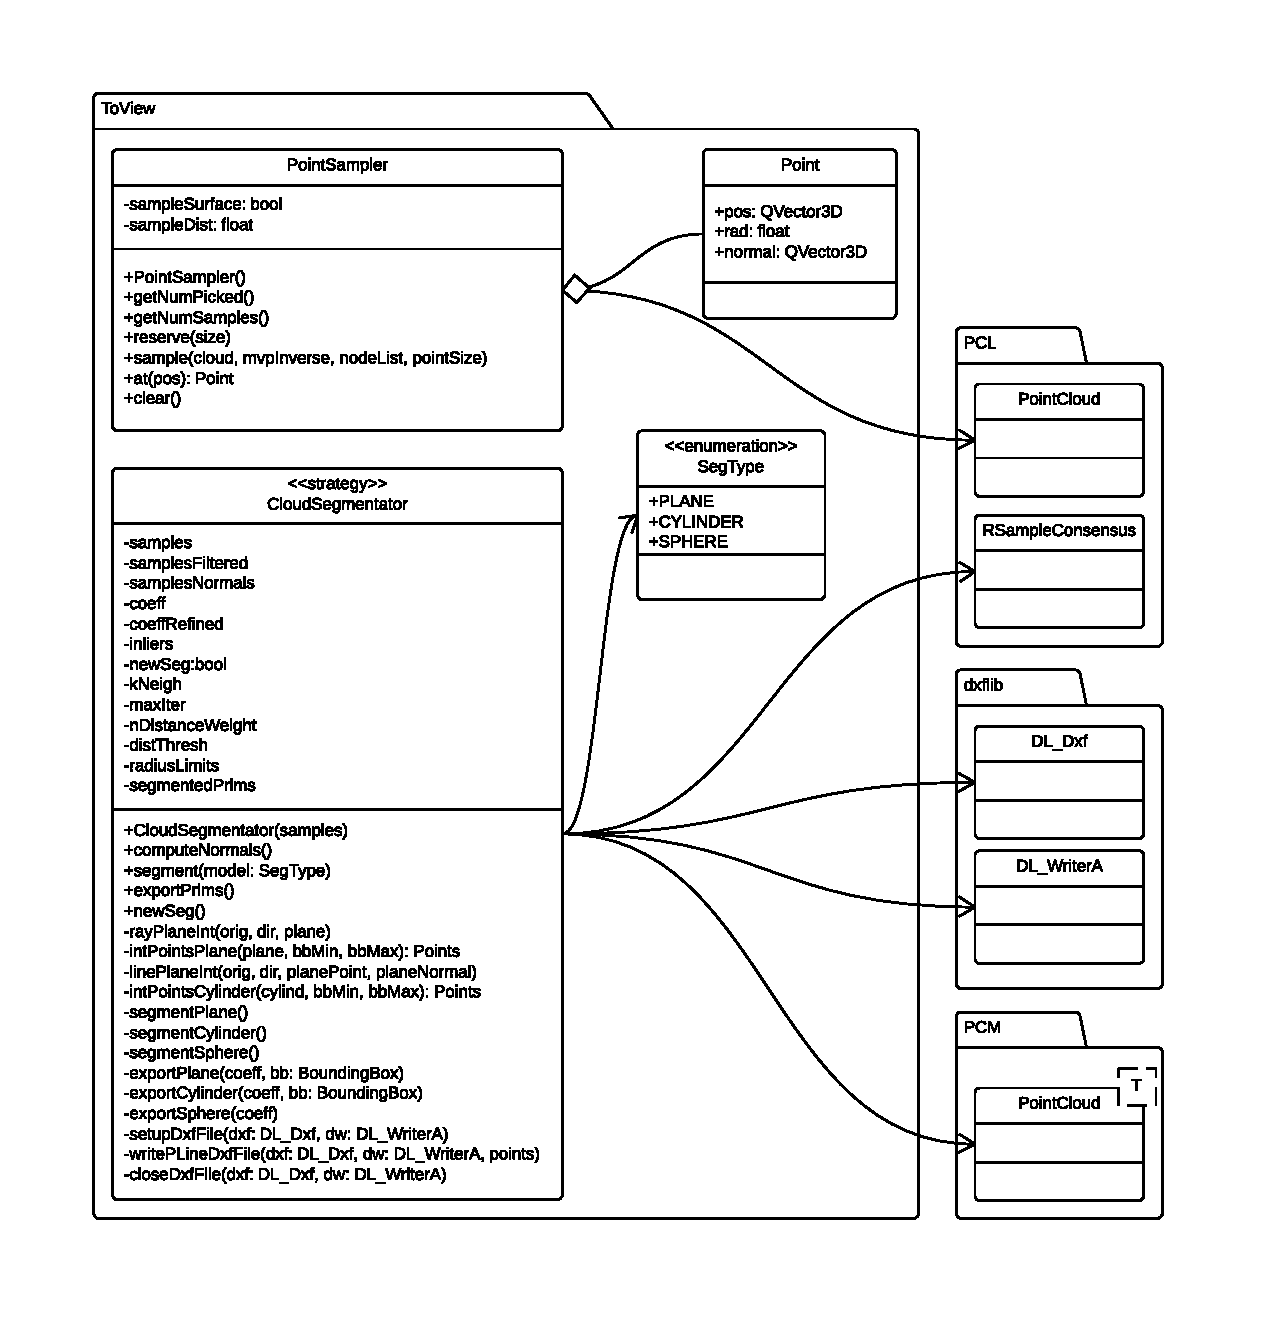
\includegraphics[scale=0.6]{figures/segmentation.pdf}
	\caption[Segmentation class diagram]{
		Class diagram of the classes related to segmentation.
	}
	\label{segmentation_class}
\end{figure}

In \autoref{segmentation_class}, the classes related to the segmentation process are detailed. One of the most significant classes is \textbf{PointSampler}, this will be the class that samples the corresponding point cloud and then converts the data so that it is compatible with PCL. It also is capable of picking individual points for distance measurements, and storing them in a similar fashion to a STL vector for quick access.   

Next, the most important class will be briefly explained. \textbf{CloudSegmentator} uses the information obtained by \textbf{PointSampler} to segment three types of primitives, \textit{planes}, \textit{cylinders} and \textit{spheres}. But this is not all the functionality that this class provides, it is also capable of exporting these primitives to an AutoCAD compatible format. 

To achieve these objectives, this class uses the \textbf{RSampleConsensus} class for primitive fitting and \textbf{DL\_Dxf} for \textit{DXF}\footnote{\textit{Drawing Exchange Format} is a CAD data file format developed by Autodesk for enabling data interoperability between AutoCAD and other programs.} exporting. Since there is not a good way to export cylinders and spheres in the DXF format, the segmentator will also support exporting these primitives as \textit{SCR}\footnote{\textit{Script Files} are simply a list of AutoCAD commands.} files.

Since some of the primitives need normals for the segmentation process, \textbf{CloudSegmentator} also includes the capability to estimate them. The pattern \textit{Strategy} was used for the design of this class so that adding primitives in the future will be easy. 

\section[Functionality]{Functionality}

The need for a robust tool to complement PCM was quickly noticed when using PCM's basic visualizer. This tool was enough for testing but left a lot to be desired, even when multiple clouds were not rendered onscreen and no advanced operations were performed on them. 

Moreover, the rendering code was written with the help of an open source scene graph called OSG\footnote{Open Scene Graph}. This was also an inconvenient because of the massive nature of the clouds that this software is designed to deal with. Heavy optimization would have to be performed and complete access to OpenGL rendering code was needed.

\begin{figure}[h]
	\centering
	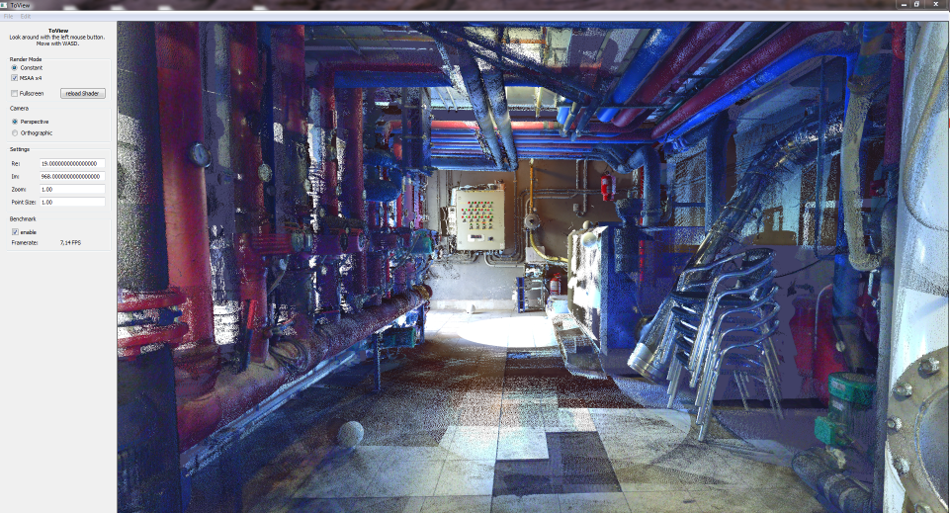
\includegraphics[scale=0.6]{figures/tovi_screen.png}
	\caption[Early ToView screenshot]{
		Screenshot showing an early version of ToView.
	}
	\label{early_toview}
\end{figure}

Furthermore, almost all of PCM's functionality was only accessible through multiple command line tools. When trying to integrate this software in engineering workflows, this was a big limitation.

If PCM was to be adopted by non-technical users, a GUI and more interactivity were essential. This is where ToView came to the rescue (see \autoref{early_toview}), with multiple cloud support, a GUI, advanced rendering, distance measuring capabilities, object detection, etc. All the functionality that ToView brings to the table will be exposed in the following subsections.

\subsection[Render modes]{Render modes}

In light of the need for high quality point based rendering, but also trying to keep versatility, three rendering modes are supported in ToView:

\begin{itemize}
	\item \textbf{Constant:} Most basic type of point-based rendering, it does not require point normals or radii.
	\item \textbf{Dynamic:} Almost the same as the previous mode, but requires point radii to reduce clipping and increase rendering quality and performance.
	\item \textbf{Perspective accurate:} Most advanced type of rendering, requires point normals and radii. This rendering mode yields high quality renders but at a greater computational cost.
\end{itemize}

\begin{figure}[h]
	\centering
	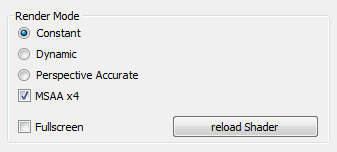
\includegraphics[scale=0.9]{figures/render_modes.png}
	\caption[Render modes]{
		Screenshot showing all of the available render modes in ToView's interface.
	}
	\label{render_modes}
\end{figure}

As we can see in \autoref{render_modes}, more parameters like anti-aliasing or full-screen rendering are also exposed through the GUI. Anti-aliasing will play a huge role in high quality rendering as it increases image quality dramatically.

All of these rendering modes and a complementary technique that was not exposed to the user in ToView, but was also implemented for testing, will be explained in depth in \autoref{chapter_7}.

\subsection[Camera types]{Camera types}

Since camera only one camera type was present in the old visualizer, two types of camera paradigms were implemented:

\begin{itemize}
	\item \textbf{First-person camera:} Type of camera that imitates how movement is implemented in video games. This camera is ideal for virtual tours of the scenes, or working with really big scenes with multiple objects.
	\item \textbf{Orbital:} This camera model emulates cameras in modeling software (Blender, AutoCAD, etc.). This camera type is optimal for working with single objects and an orthographic projection.
\end{itemize}

Furthermore, because of the engineering nature of our software, a perspective camera may not be the optimal choice. This is the reason why two types of projection are available for the user:

\begin{itemize}
	\item \textbf{Perspective:} Projection model that reflects how the human eye perceives scenes, objects in the distance appear smaller than objects close by. This projection type is useful when moving through a city or interior datasets. 
	\item \textbf{Ortographic:} This projection type ignores the aforementioned effect so that to-scale modeling can occur. This projection model is useful when working with single objects or when we need to see parallel lines as parallel in the final image.
\end{itemize}

All of these camera types are controlled using the keyboard and mouse, trying to make it as easy as possible for the end user. The math and implementation details behind these cameras are explained in \autoref{camera_model}. The options are exposed to the user through a convenient menu in the interface and do not require restarting the application to be applied (see \autoref{camera_types}).

\begin{figure}[h]
	\centering
	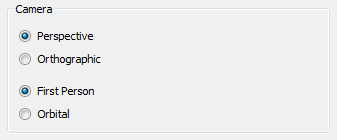
\includegraphics[scale=0.9]{figures/camera_types.png}
	\caption[Camera options]{
		Screenshot showing all of the available camera options in ToView's interface.
	}
	\label{camera_types}
\end{figure}

\subsection[Preprocessing]{Preprocessing}

As mentioned before, scanners sometimes output clouds that may not be optimal for the task at hand. As a consequence, some preprocessing can be needed. ToView offers its users several operations:

\begin{itemize}
	\item \textbf{Voxel grid filter:} Downsampling filter, useful to thin dense point clouds or keep the cloud density uniform. 
	\item \textbf{Statistical outlier removal:} Noise removal filter, it can be used to remove outliers or noise present in the clouds.
	\item \textbf{Radii estimation:} Necessary process if the end user wants to use the two advanced rendering modes. It estimates the value of the point radii.
	\item \textbf{K-d tree building:} Essential process for the visualization of the point clouds. Without a spatial acceleration structure, the clouds would be too big to render or perform any operation.
\end{itemize}

The preprocessing filters are further explained in \autoref{chapter_9}. All of these point cloud operations are exposed to the user through the tools menu in the interface(see \autoref{tools_menu}).

\begin{figure}[h]
	\centering
	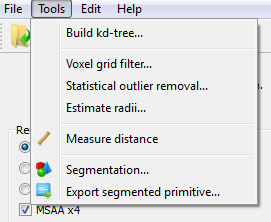
\includegraphics[scale=0.7]{figures/tools.png}
	\caption[Tools menu]{
		Screenshot showing all of the available point cloud tools in ToView's interface.
	}
	\label{tools_menu}
\end{figure}

\subsection[Cloud interaction]{Cloud interaction}

One of the main drawbacks of having a simple visualizer without a GUI was the inability to integrate multiple point clouds, and perform modifications on the clouds (see \autoref{mult_clouds}). 

\begin{figure}[h]
	\centering
	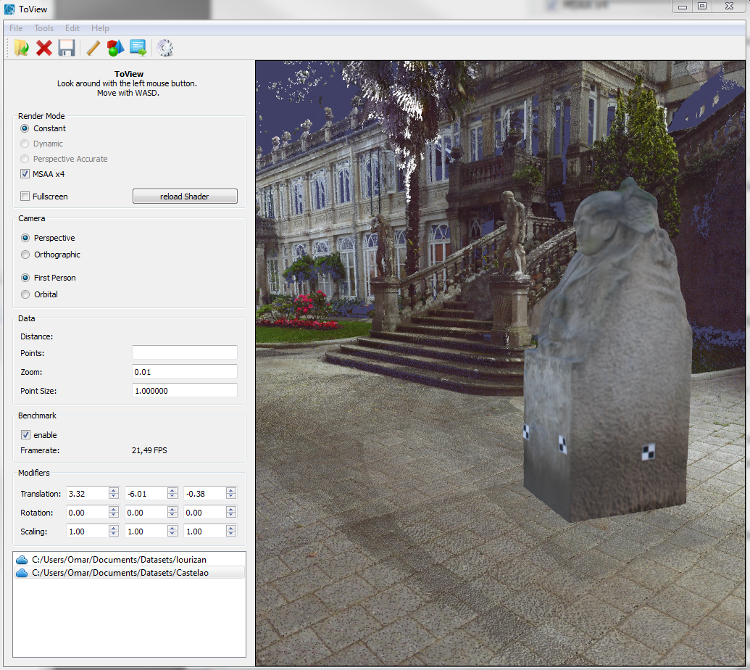
\includegraphics[scale=0.495]{figures/mult_clouds_int.png}
	\caption[Multiple point cloud integration]{
		Two clouds (a park and a statue) integrated using ToView.
	}
	\label{mult_clouds}
\end{figure}

ToView offers multiple possibilities on this front:

\begin{itemize}
	\item \textbf{Point cloud transformation:} Each cloud can be transformed to the user's liking. 
	\begin{itemize}
		\item \textbf{Translation:} The cloud can be moved through space.
		\item \textbf{Rotation:} The cloud can be rotated.
		\item \textbf{Scaling:} The cloud can be transformed to be bigger or smaller.
	\end{itemize}
	\item \textbf{Multiple point cloud integration:} The user can transform multiple clouds at the same time. This allows the integration of multiple point clouds, correcting positioning errors, wrong coordinate systems, etc.
	\item \textbf{Cloud selector:} Select a cloud to transform, eliminate or perform any operation in an easy way through the interface.
\end{itemize}

The aforementioned features are exposed through the interface in a panel in the interface (see \autoref{cloud_modifiers}). All of these features work in real-time, allowing the user to see the changes made reflected instantly. Clouds can also be added or removed in real-time according to the user's needs.   

\begin{figure}[h]
	\centering
	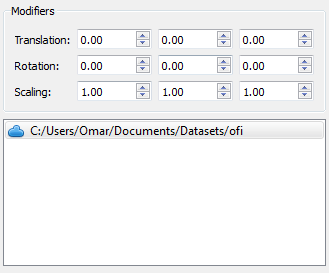
\includegraphics[scale=0.7]{figures/cloud_modif.png}
	\caption[Cloud interaction]{
		Screenshot showing the cloud interaction menu in ToView's interface.
	}
	\label{cloud_modifiers}
\end{figure}

\subsection[Point picking]{Point picking}

In order to be able to measure distances or segment primitives interactively in the clouds, the visualizer has to be capable of finding the correct point that the user desires in the clouds. This action is called point picking, and is performed in real-time by the visualizer. 

To achieve this, the first step is getting the position the user has clicked in the window. This is done using QT's API and returns two values, the $x$ and $y$ coordinates.

Secondly, the coordinates are transformed so that we have the coordinates of a ray corresponding to that pixel in NDC. The ray origin can be obtained with the following equation:

\begin{equation} \mathbf{r_{start}} = ((x/w - 0.5) * 2, (y/h - 0.5) * 2, 0) \end{equation} 

Being $w$ the width of the window and $h$ the height. The ray end can be obtained with the equation that follows:

\begin{equation} \mathbf{r_{end}} = ((x/w - 0.5) * 2, (y/h - 0.5) * 2, 1) \end{equation} 

Once we have the ray in NDC space, we need to transform it to world space. The operation needed to get the ray in world space is just a matrix multiplication:

\begin{equation} \mathbf{r_{world}} = \textbf{\textit{MVP}}^{-1} \cdot \mathbf{r_{ndc}} \end{equation}

Finally, after the ray in world coordinates is obtained, it is just a matter of obtaining the points that intersect with the ray and return the closest to the viewpoint.

\subsection[Distance measurements]{Distance measurements}

\subsection[Primitive segmentation]{Primitive segmentation}

\subsection[Primitive exportation]{Primitive exportation}

\section[Results]{Results}


	%
% T�TULO DEL CAP�TULO
%
\chapter[Advanced GPU point rendering]{
	Advanced GPU point rendering
	\label{chapter_7}
}

The first approaches to point rendering like \cite{surfsplat} were CPU based, this was clearly not the right approach for real-time point rendering. To increase performance, the massively parallel computing power of GPUs should be taken advantage of. In a similar fashion to how triangle meshes are rendered nowadays, we will offload rendering to the graphics hardware freeing the CPU to perform other tasks. This will provide much higher performance than a CPU based solution. 

This would seem an easy task at first sight, but due to missing point splat support in graphics hardware; exploiting the GPU's hardware acceleration for point-based rendering is not an straightforward task. Fortunately, thanks to the introduction of fragment and vertex shaders, we will be able to use the hardware for this job using custom shaders.

\section[Performance details]{Performance details}

One of the reasons why point-based rendering is used, is the huge complexity of today's datasets (more than 1KM points), that can be acquired by LiDAR scanners. When these models are rendered, a triangle may only cover a few or not even one pixel. Since the triangle rasterization setup in this cases does not pay off, rendering massive triangle meshes is not efficient.

In these cases, is where points seem to be the more suited rendering primitive. But, when rendering massive point clouds, we should use the following guidelines:

\begin{itemize}
\item \textbf{Interleaved vertex arrays:} To minimize the number of calls to the OpenGL API, the point data (positions \textbf{p}, colors \textbf{c}, radii \textbf{r}, normals \textbf{n}, etc.) has to be stored in one large array. Thanks to this, we can render the points with just one call to \textit{glDrawArrays()}. For better memory coherence, the data should also be stored in an interleaved manner (i.e. $[\textbf{p}_{1},\textbf{p}_{2},\ldots,\textbf{c}_{1},\textbf{c}_{2},\ldots]$).
\item \textbf{Vertex Buffer Objects:} In each frame, all the point data has to be transferred to the GPU. This would quickly become a bottleneck in massive datasets. Since sometimes this data will be static for several frames, it will be stored in high performance video memory for efficient GPU access. VBOs are the standard way of achieving our objective since OpenGL version 1.5 (2003).
\item \textbf{Optimum VBO size:} The VBO size will be kept in the optimum range recommended by NVIDIA (1-4 MB). If chunks are larger than that, they will be split in several VBOs. 
\item \textbf{Data formats:} In order to reduce the GPU memory consumed, and decrease transfer costs, the point data will be stored in a compact format. Position and normals will be stored using single-precision floating-point numbers, colors will be stored using just 4 bytes (one per RGBA channel). 
\item \textbf{Shading language:} Low-level shading languages offer a small performance advantage, but since nowadays it is marginal, GLSL will be used for shader programming. High-level languages like GLSL are more convenient to use and way less problematic when adding features or reviewing the code.
\end{itemize} 

All of these optimization techniques are valid for all the point rendering approaches that will be explained next. 

\section[Splat rasterization]{Splat rasterization}

This is the first step in splat rendering, it determines the pixels that a point will cover. Since there are no splat primitives, splats have to be created from other rendering primitives, like points or triangles. All of the following methods were implemented and tested in modern OpenGL, the code can be reviewed in the repository of the project (\url{http://tovias.citic.udc.es/}). 

\subsection[Image-aligned squares]{Image-aligned squares}

For the highest performance, splats should be rendered using only one OpenGL point for each splat, using:
\\
\lstset{emph={[2]glDrawArrays}, emphstyle={[2]\color{PineGreen}},emph={[3]GL_POINTS}, emphstyle={[3]\color{RawSienna}}}
\begin{lstlisting}[caption={Draw call to draw a set of splats.},captionpos=b]
 glDrawArrays(GL_POINTS, 0, VBOSize);
\end{lstlisting}

An optional output of a vertex shader is the point size, that when set to $s$, creates a image-space square of $s \times s$ pixels centered in the vertex position. Instead of squares, image aligned circles can be rendered by enabling point smoothing and MSAA:
\\
\lstset{emph={[2]glEnable}, emphstyle={[2]\color{PineGreen}},emph={[3]GL_POINT_SMOOTH}, emphstyle={[3]\color{RawSienna}}}
\begin{lstlisting}[caption={OpenGL flag needed for point smoothing.},captionpos=b]
 glEnable(GL_POINT_SMOOTH);
\end{lstlisting}

The screen-space size of the projected OpenGL point has to be adjusted in the vertex shader, so that holes do not appear when moving closer to the object. To allow us to modify the point size dynamically in the vertex shader and specify our coordinate system origin, we will use the following code:
\\
\lstset{emph={[2]glEnable,glPointParameteri}, emphstyle={[2]\color{PineGreen}},emph={[3]GL_PROGRAM_POINT_SIZE,GL_POINT_SPRITE_COORD_ORIGIN,GL_LOWER_LEFT}, 
		emphstyle={[3]\color{RawSienna}}}
\begin{lstlisting}[caption={Flags needed for changing the point size in a vertex shader.},captionpos=b]
 glEnable(GL_PROGRAM_POINT_SIZE);
 glPointParameteri(GL_POINT_SPRITE_COORD_ORIGIN, GL_LOWER_LEFT);
\end{lstlisting}

The adjusted point size is approximated by calculating the foreshortening of the point radii $r$, depending on the point position $\mathbf{p}$ in camera coordinates:

\begin{equation} s = 1.5\cdot r\cdot \frac{n}{p_{z}}\cdot \frac{h}{t-b} \end{equation}

Where $n$, $t$ and $b$ are the near/top/bottom parameters of the camera's view frustum and $h$ the height of the viewport in pixels. The advantage of this rasterization method, is that because of its simplicity, it is the fastest of the three studied methods. It is also the one that requires the least amount of information, since it only needs the splat position, color and optionally radius. 

\begin{figure}[h]
	\centering
	
\includegraphics[scale=0.5]{figures/squares.png}
	\caption[Image aligned squares defects]{
		Render image showing the defects that image-aligned squares present in object contours.
	}
	\label{squares}
\end{figure}

However, this method is not optimal for high quality rendering. It yields bad results specially near the object's contour (see \autoref{squares}), where the poor approximation of the splat shape is specially noticeable. Furthermore, since all fragments created with this technique have the same depth value, this prevents the correct blending of overlapping splats.

\subsection[Affinely projected point sprites]{Affinely projected point sprites}

An improved approximation to the true splat shape is the one in \cite{circularsplats}, this technique was called circular object-space splats. It starts by adjusting the point size in the vertex shader as in the previous method, but for each of the squares, the fragment shader will determine whether or not the fragment corresponds to the inside or outside of the splat. 

Fragments outside the splat will be discarded using the \textit{discard} GLSL command. This will result in circular splat rasterization. For this technique to work we will have to activate the following feature in OpenGL:
\\
\lstset{emph={[2]glEnable}, emphstyle={[2]\color{PineGreen}},emph={[3]GL_POINT_SPRITE}, 
		emphstyle={[3]\color{RawSienna}}}
\begin{lstlisting}[caption={Flag needed to discard fragments in fragment shader.},captionpos=b]
 glEnable(GL_POINT_SPRITE);
\end{lstlisting} 

Next, we need to parameterize the screen-space square in the range $[-r,r]^2$, being $r$ the splat radius. For each of its fragments $(x,y) \in [-r,r]^2$, a depth offset $\delta z$ from the splat center $\mathbf{p}$ can be computed as a linear function that depends on the camera-space normal vector $\mathbf{n} = (n_{x},n_{y},n_{z})$:

\begin{equation}\label{eq:depth} \delta z = -\frac{n_{x}}{n_{z}} \cdot x - \frac{n_{y}}{n_{z}} \cdot y \end{equation}

The depth offset can after this step be used to compute the 3D distance to the splat center. This distance can then be used to check whether a the fragment corresponds to the inside of the splat or not with:

\begin{equation} \left \| (x,y,\delta z) \right \| \leq r \end{equation}

Since one of the problems that we found in the image-aligned squares was the lack of a depth value for the splat, the depth offset $\delta z$ should also be used to correct the fragment's depth value. Starting from the camera space depth value $z' = p_{z} + \delta z$, the frustum and viewport transformations allow us to calculate the window-space depth buffer entry, from the far plane $f$ and the near plane $n$:

\begin{equation}\label{eq:zbuffer} \text{zbuffer}(x,y) = \frac{1}{z'} \cdot \frac{fn}{f-n} \cdot \frac{f}{f-n} \end{equation} 

This approach yields much better results in comparison to the previous one, this is specially apparent in object contours. But it does not come without its share of issues. Since the depth offset is just an approximation due to the fact that in the \autoref{eq:depth} a parallel projection is assumed. Thus neglecting the angle between the viewing ray and the splat normal. This creates artifacts when viewing the splat from extreme angles (see \autoref{ext_angles}).

\begin{figure}[h]
	\centering
	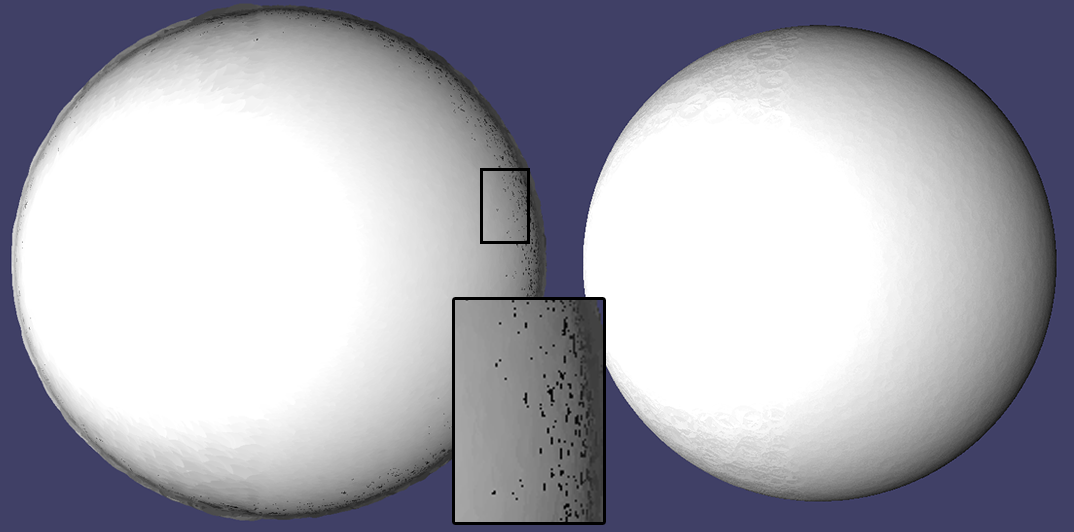
\includegraphics[scale=0.35]{figures/comp_perps2.png}
	\caption[Comparison between affinely projected and perspectively accurate rasterization]{
		Local affine approximations can cause holes for extreme viewing angles (\textbf{left}). This problem is taken care of by using perspectively correct rasterization (\textbf{right}).
	}
	\label{ext_angles}
\end{figure}

\subsection[Perspectively correct rasterization]{Perspectively correct rasterization}

The last approximation was able to correctly transform the splat center, but failed to do the same with the contour, this caused holes to appear in the rendered image. This is why, to create a perspective correct approximation, the technique in \cite{perspcorrect} was created. In this method, the outer contour of the splat was correctly transformed, but had projective errors in the splat center. This approach had a high computational cost, that made it very costly.

\begin{figure}[h]
	\centering
	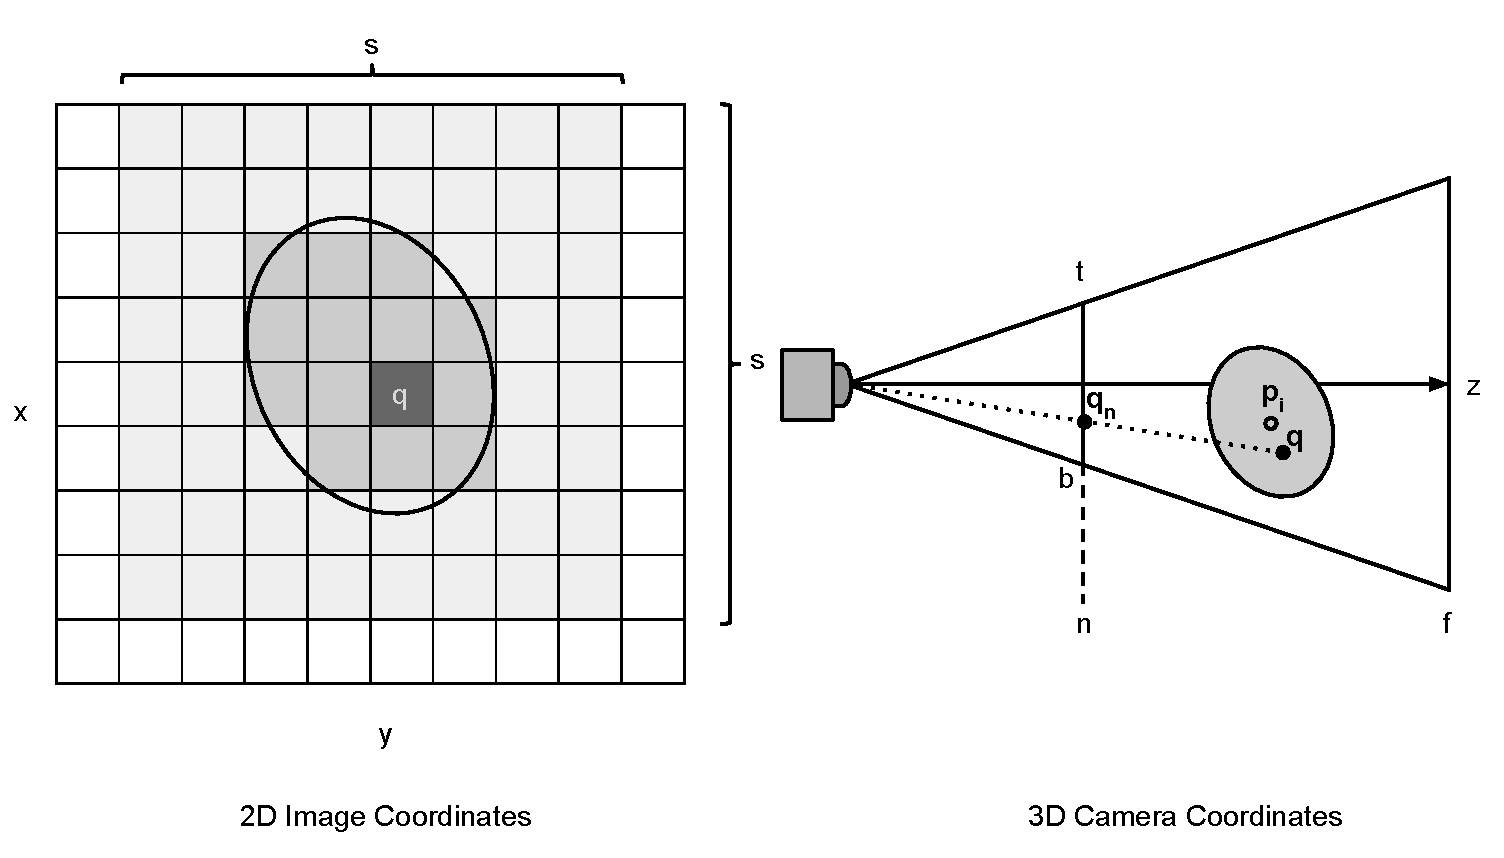
\includegraphics[scale=0.5]{figures/persp_accu.pdf}
	\caption[Perspective accurate]{
		Projection of the splat and raycasting visual explanation.
	}
	\label{persp_accu}
\end{figure}

A more efficient while being perspective correct technique was presented in \cite{perspeffi}. The main concept in this method is to determine the 3D point corresponding to a 2D fragment based on local raycasting. This method can also handle elliptical splats, although we will concentrate our efforts in circular splats since this is our case study.

A splat $s_{i}$ is represented by a center $\mathbf{p_{i}}$, a radius $r_{i}$ and its normal $\mathbf{n_{i}}$. We start by rendering the splats again with \textit{GL\_POINTS} and the pixel size given by the splat radius. Next, for each fragment $(x,y)$ the \textit{exact} corresponding 3D point $\mathbf{q}$ is computed using local raycasting (see \autoref{persp_accu}). With this point $\mathbf{q}$, the distance to the center of the splat is computed, if the fragment lies outside of the splat it is discarded with the \textit{discard} command. The \autoref{eq:dist} dictates if the fragment is outside or inside the splat:

\begin{equation}\label{eq:dist} \left \| \mathbf{q} - \mathbf{p_{i}} \right \| \leq r \end{equation} 

To compute $\mathbf{q}$ we will first need to invert the window-to-viewport transformation, mapping the fragment $(x,y)$ to a 3D point $\mathbf{q_{n}}$ on the near plane:

\begin{equation} 
\mathbf{q_{n}} = 
\begin{pmatrix}
x\cdot \frac{r-l}{w}-\frac{r-l}{2}
\\
y\cdot \frac{t-b}{h}-\frac{t-b}{2}
\\ 
-n
\end{pmatrix} 
\end{equation}  

Being $b$/$t$/$l$/$r$ the bottom/top/left/right corners of the frustum and $w$/$h$ the width/height of the viewport. Casting a ray from the origin through the point $\mathbf{q_{n}}$ and intersecting with the splats supporting plane will yield the necessary point $\mathbf{q}$. First we will calculate the distance at which the ray intersects the plane:

\begin{equation} t = \frac{\mathbf{p_{i}} \cdot \mathbf{n_{i}}}{\mathbf{q_{n} \cdot \mathbf{n_{i}}}} \end{equation}  

Once the distance $t$ is obtained, the point $\mathbf{q}$ is easily obtained with the following equation:

\begin{equation} \mathbf{q} = t\mathbf{q_{n}} \end{equation}  

After the point $\mathbf{q}$ is known, we can apply \autoref{eq:dist} to test whether the fragment falls inside the splat or not. Of course, we will not be done until we adjust the new fragment depth value using $q_{z}$ as $z'$ in \autoref{eq:zbuffer}. Since the 3D point $\mathbf{q}$ is the \textit{exact} preimage of the projective transform, this means that this method is perspectively correct for each pixel. 

\begin{figure}[h]
	\centering
	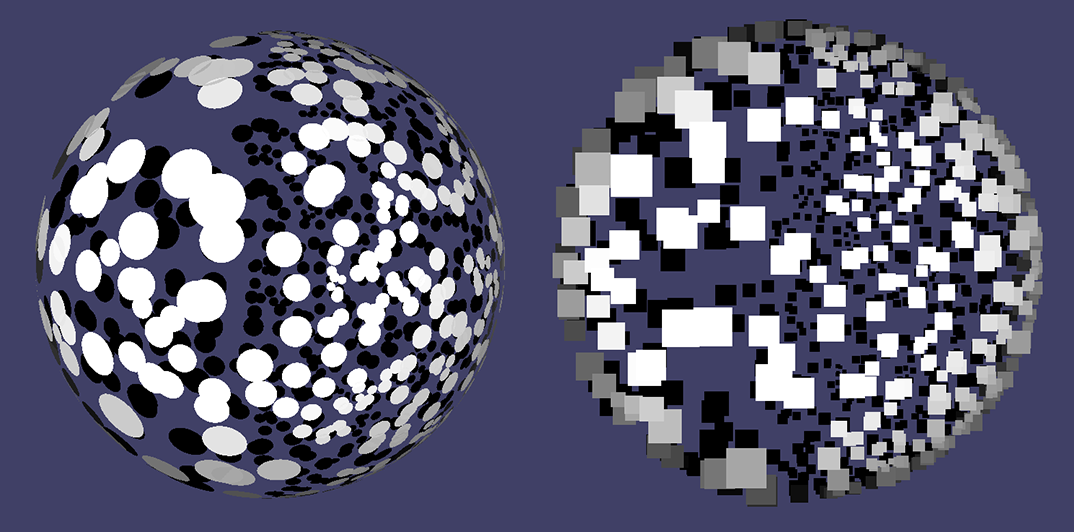
\includegraphics[scale=0.35]{figures/comp_squares.png}
	\caption[Comparison between perspectively accurate rasterization and image-aligned squares]{
		Perspectively correct rasterization represents the splat with a lot more fidelity than the initial technique, specially in the object contour (\textbf{left}).  Image-aligned squares centered in the splat position (\textbf{right}).
	}
	\label{comp_squares}
\end{figure} 

\section[Antialiasing]{Antialiasing}

The chosen method to remove anti-aliasing artifacts in the visualizer was \textbf{MSAA} \cite{realtime}. The term usually refers to a special case of super-sampling. If the reader wants more information about super-sampling, feel free to check \cite{BDE}, SSAA was the anti-aliasing method used in that point-based rendering engine. That type of anti-aliasing works well in offline rendering, but for real-time rendering it is not a good option because of its computational cost.

\begin{figure}[h]
	\centering
	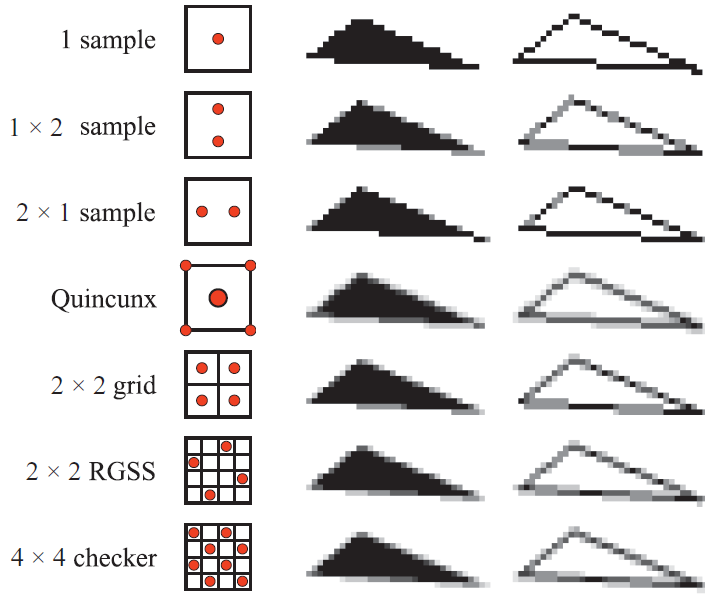
\includegraphics[scale=0.35]{figures/supersampling_patterns.png}
	\caption[Typical super-sampling patterns]{
		A series of typical super-sampling patterns applied to a triangle. Aliasing is reduced even when the resolution is not increased. Source: \cite{realtime}.
	}
	\label{ssaa_patterns}
\end{figure}

One way to reduce aliasing artifacts is through \textit{oversampling}. Oversampling is the process of sampling a signal at a rate that is higher than the desired output. In the case of images this results in a reduction in the aliasing artifacts. When this is applied to graphics or 2D images we call it SSAA. We can apply lots of different super-sampling patterns and each one will yield a different result(see \autoref{ssaa_patterns}).    

\begin{figure}[h]
	\centering
	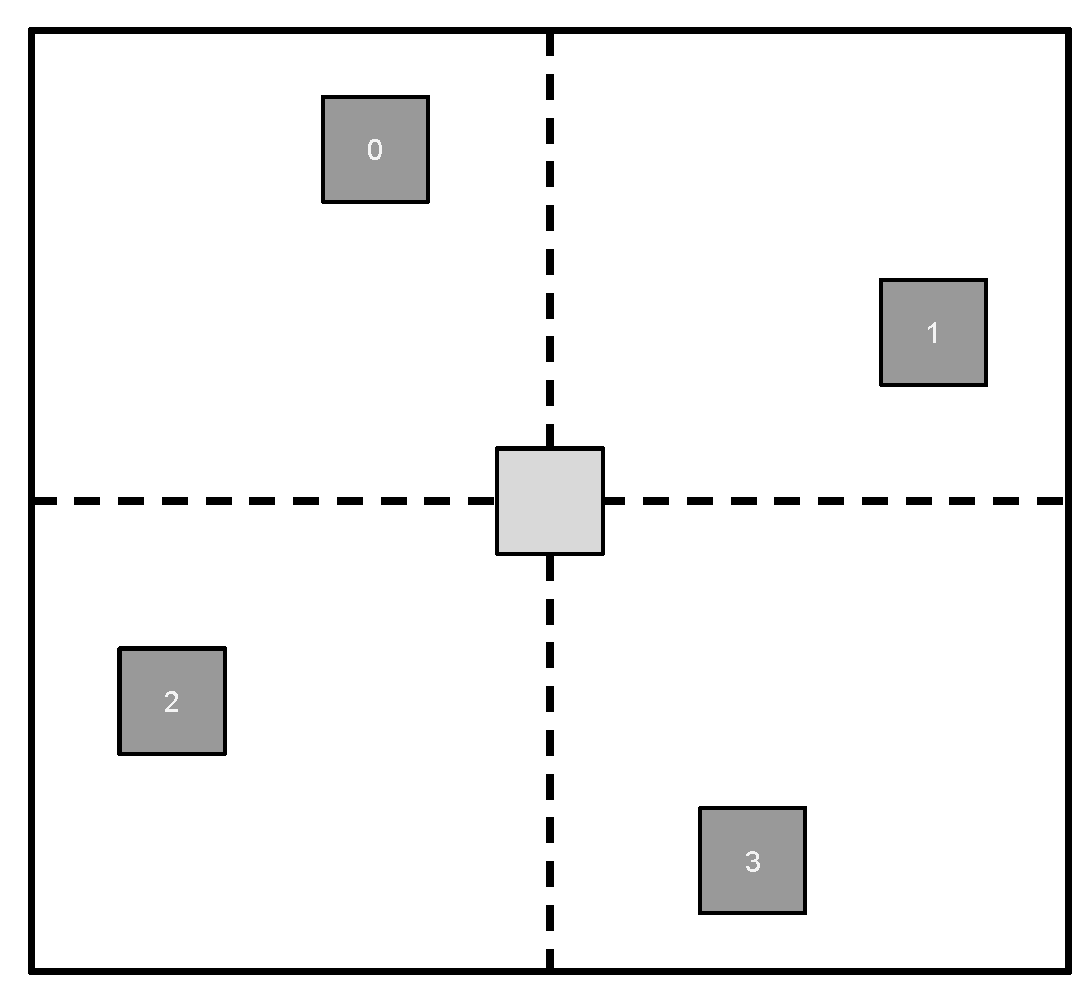
\includegraphics[scale=0.28]{figures/typ_samp.pdf}
	\caption[MSAA subsample placement for a rotated grid pattern]{
		Subsample placement for a MSAA x4 rotated grid pattern.
	}
	\label{msaa_typ}
\end{figure}

In order to keep most of the benefits of SSAA without the performance penalty. Seeing that aliasing only occurs in the borders of geometric primitives, we will exploit this fact in our advantage. MSAA works in a similar manner to SSAA, the coverage and occlusion tests are performed at a higher sampling rate (from x2 to x16). For coverage, we have N samples within a pixel, where N is the multi-sample rate. A typical MSAA sample pattern can be observed in \autoref{msaa_typ}.  

With the sample points the primitive is tested for coverage building a \textit{coverage mask}. For occlusion testing, the primitive depth is interpolated at each sub-sample. Where MSAA starts differing from SSAA is in the pixel shader. It is not executed for each sub-sample, but once for each pixel with a coverage mask that is not zero. This means that the shader cost is not as big as with SSAA. When a pixel shader outputs a value, the value will be written only if both the coverage and depth tests are passed (see \autoref{msaa_cover}).  

\begin{figure}[h]
	\centering
	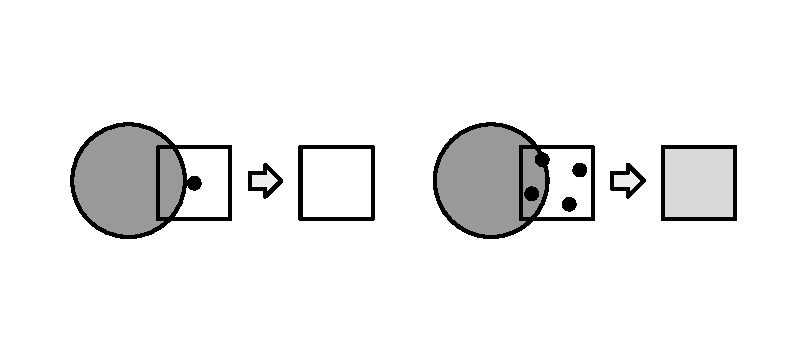
\includegraphics[scale=1]{figures/msaa_cover.pdf}
	\caption[MSAA and non-MSAA results for a partially covered point]{
		Non-MSAA rendering does not support partially covered primitives and in this case would not color the pixel (\textbf{left}).  MSAA rendering on the other hand would detect that some subsamples are covered and would average an output color from all the subsamples (\textbf{right}).
	}
	\label{msaa_cover}
\end{figure}      

Once we have the oversampled signal, we have to resample it to the target resolution before it can be displayed. In MSAA this process is called \textit{resolving} the render target. In the early days of MSAA, the resolve process was carried out in the GPU's hardware, using a one pixel wide box filter. Which in essence is the same as averaging all the subsamples of a given pixel. 

As programmable shaders arrived, we now have the possibility to perform the MSAA resolve in a custom shader. In this project this step was not deemed a priority and we have relied on the OpenGL API to perform it. But, these are not the only advantages, bandwidth usage is also improved when using MSAA versus SSAA. Since the pixel shader is only executed once per pixel, as a result the same value is often written to all the subsamples of the render target. GPUs can take advantage of this factor sending not only the pixel value, but the number of samples that have to be written, which in term is a form of loss-less compression. 


Summing up, the use of MSAA has given us an increase in image quality without a big impact in performance. This increase in rendering quality is specially noticeable in dynamic cases, but can also be observed in static images (see \autoref{msaa_comp}).  

\begin{figure}[h]
	\centering
	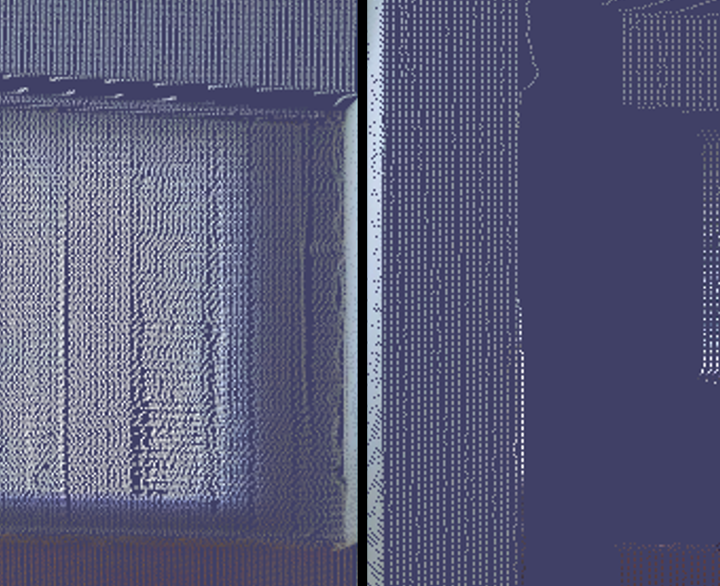
\includegraphics[scale=0.5]{figures/msaa_comp.png}
	\caption[MSAA and non-MSAA result comparison]{
	MSAA rendering obtains smoother surfaces without holes and less edge aliasing (\textbf{left}). Non-MSAA rendering results in holes and non-smooth edge gradients (\textbf{right}).
	}
	\label{msaa_comp}
\end{figure} 

	%
% T�TULO DEL CAP�TULO
%
\chapter{Object detection: RANSAC
	\label{chapter_8}
}

RANSAC is an abbreviation for ``RANdom SAmple Consensus''. This is an iterative method to estimate parameters of a mathematical model from a set of observed points which can contain outliers. This is a non-deterministic algorithm, since we are not able to guarantee that it will produce a correct result. The probability of reaching a reasonable result will improve as the number of iterations increases. The algorithm was first published in \cite{ransac}.

The basic assumption is that the data contains \textit{inliers}\footnote{Data whose distribution can be estimated by some model.}, though it may contain noise and \textit{outliers}\footnote{Data that does not fit the model.}. Outliers can come from errors or imprecise measurements, extreme values of noise, etc. RANSAC assumes that given a set of inliers, there should exist a procedure that can estimate the unknown parameters of a model that will fit this data (see \autoref{RANSAC}).

\begin{figure}[h]
	\centering
	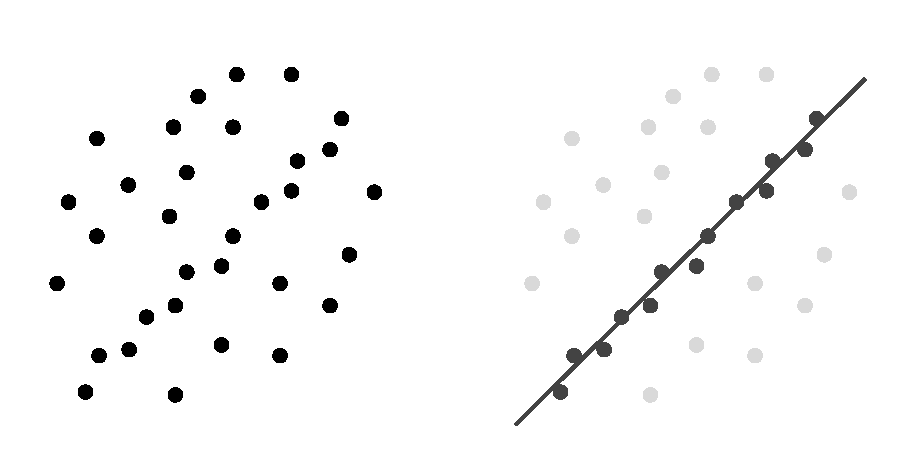
\includegraphics[scale=0.8]{figures/RANSAC.pdf}
	\caption[RANSAC example]{
		A set of points with many inliers in which a line is to be fitted (\textbf{left}).  Resulting fitted line using RANSAC, in which outliers have no influence in the result (\textbf{right}).
	}
	\label{RANSAC}
\end{figure}

\section[Original algorithm]{Original algorithm}

Unlike other estimation techniques, RANSAC generates candidate solutions using the minimum number of points required to fit the model parameters. RANSAC instead of using as much of the data as possible and then eliminate the outliers, uses the smallest set possible and then tries to enlarge this subset with coherent points. The basic algorithm can be summed up in the following steps: 

\begin{enumerate}
	\item Select randomly the minimum subset of points to determine the model parameters.
	\item Solve for the parameters of the model (i.e. with a least squares method).
	\item Test how many points from the complete dataset fit with a predefined tolerance $\epsilon$.
	\item If the fraction of inliers over the total number of points is sufficiently good, then the model is re-estimated (since it was only estimated using the initial inliers).
	\item Finally, the model is evaluated by estimating the error of the inliers relative to the model.
\end{enumerate}

This procedure is repeated a certain number of times, each time producing either a new model which is either rejected because too few points are classified as inliers or a better model together with its error measure. In the latter case, we keep the refined model if its error is lower than the last saved model.

The algorithm will stop when it reaches $N$ iterations or when the model reaches a desired error measure. $N$ can be calculated to ensure that the probability $p$ (usually 0.99) of one of the subsets of random samples will not contain an outlier. Being $u$ the probability that any selected point is an inlier and $v = 1 - u$ the probability of observing an outlier. $N$ iterations of the minimum number of points $m$ are required:

\begin{equation} 1 - p = (1 - u^m)^N \end{equation}

After solving for $N$ we will obtain the necessary number of iterations:

\begin{equation} N = \frac{log(1 - p)}{log(1 - (1 - v) ^ m)} \end{equation}

Since our objective is estimating primitives in real-time, we will let the user choose this parameter so that computational time is not too high.

An advantage of RANSAC is the robust estimation of the model parameters (it can estimate the parameters even when a significant number of outliers is present). But, a disadvantage of RANSAC is that there is no upper bound on the time that it would take to compute the correct model parameters. Another disadvantage is that it can only estimate one model at a time, if two or more instances of the model exist, RANSAC will fail to find either of them.

\section[Alternative algorithms]{Alternative algorithms}

Since 1981 RANSAC has become one of the most widely used tools in computer vision. Since then, there have been several variations of the algorithm meant to improve its robustness, speed and accuracy. Some of the improved algorithms will be briefly described in this section.

\subsection[MSAC and MLESAC]{MSAC and MLESAC}

In the original algorithm, if the threshold $\epsilon$ is too high, the robust estimate can be very poor. This happens because RANSAC finds the minimum of a cost function:

\begin{equation} C = \sum_{i} p(e_{i}^2) \end{equation}

Where $p(e^2)$ is:

\begin{equation} 
p(e^2) = \left\{\begin{matrix}
0 & e^2 < \epsilon^2\\ 
constant & e^2 \geq  \epsilon^2
\end{matrix}\right. 
\end{equation}

As we can see in the equations, inliers will score nothing and each outlier will score a constant penalty. As $\epsilon^2$ is higher, more solutions with the same value $C$ will appear, leading to worse estimations. In \cite{robustparam} it is shown that this can be avoided changing $C$ for:

\begin{equation} C_{2} = \sum_{i} p_{2}(e_{i}^2) \end{equation}

Where $p_{2}(e^2)$ is:

\begin{equation} 
p_{2}(e^2) = \left\{\begin{matrix}
e^2 & e^2 < \epsilon^2\\ 
\epsilon^2 & e^2 \geq  \epsilon^2
\end{matrix}\right. 
\end{equation}

This is known as a re-descending M-estimator. Outliers are still given a constant penalty, but now inliers are scored depending on how well they fit the data. The implementation of this method is called MSAC\footnote{M-Estimator Sample Consensus}.

The definition of a maximum likelihood error, will allow to further improve the results of this new technique. This improved technique is called MLESAC\footnote{Maximum Likelihood Sample Consensus} \cite{MLESAC}. The improved algorithm steps are:

\begin{enumerate}
	\item Get the minimum number of samples that will satisfy the model criteria.
	\item Search for inliers.
	\item Calculate distances to the model.
	\item Use Expectation-Maximization to find out the right value for the penalty.
	\item If the fraction of inliers over the total number of points is sufficiently good, then the model is re-estimated (since it was only estimated using the initial inliers).
	\item Finally, the model is evaluated by estimating the error of the inliers relative to the model.
\end{enumerate}
 
It can be seen that MSAC and MLESAC outperform the other two estimators, providing a $5 - 10\%$ improvement according to \cite{MLESAC}.

\subsection[PROSAC]{PROSAC}

PROSAC\footnote{Progressive Sample Consensus} is a new robust method, that exploits the linear ordering in a set of candidates using a similarity function for this purpose \cite{PROSAC}. On one hand, RANSAC normally treats all correspondences as equals and drawing uniform random samples from the dataset. On the other hand, PROSAC samples are drawn from progressively bigger sets of the best ranked candidates.

Usually, RANSAC will generate $N$ candidates. The set of $\varepsilon$ candidates, will contain a now unknown number of inliers $I$. The RANSAC loop is terminated when the probability of finding a better solution falls under a predetermined threshold. The average number of samples drawn is proportional to $(N/I)^m$. This method will be less expensive computationally than the original RANSAC, by using the linear order in $\varepsilon$. The set of candidates is obtained evaluating a similarity function $q(\cdot)$. After this step, the candidates are ordered according to the quality function. The algorithm will evaluate $N$ candidates like RANSAC, but it will do it in a different order, the samples that are of higher quality (less contaminated) will be examined first. The function chosen $q(\cdot)$ can be the Euclidean distance or any other similarity metric. 

The algorithm steps are in this case:

\begin{enumerate}
	\item Choose the hypothesis generation set.
	\item Generate hypothesis using random sampling (drawn from the subset of high quality data).
	\item Search for inliers using the estimated model.
	\item Model verification.
	\item If the probability of finding a better solution falls below a threshold terminate.
\end{enumerate}

According to \cite{PROSAC}, PROSAC is more than a hundred times faster than RANSAC in non-trivial cases.

\subsection[RRANSAC]{RRANSAC}

Typically, RANSAC will spend a lot of computational resources evaluating a large number of erroneous candidate models. These erroneous models will only fit a small subset of the complete dataset. This fact is exploited in \cite{RRANSAC} to create RRANSAC and significantly increase the speed of the original algorithm. 

The main concept in this technique, is that the efficiency of the algorithm will be improved substantially when the hypothesis evaluation step is randomized. What this means, is that because most of the hypothesis are influenced by outliers, testing a small number of points $d$ from the total $N$ ($d \ll N$) will suffice to discard the bad solution.

This idea is implemented in a two-step evaluation procedure. First, a statistical test is performed on $d$ randomly selected data points. Second, the evaluation of all the points in the dataset is only performed if the pre-test is passed. The preverification test is called the $T_{d,d}$ test, and is passed only when $d$ data points out of $d$ randomly selected are consistent with the hypothesis. 

The only remaining task is knowing the optimal value of $d$. The following equation will yield that value:

\begin{equation} d^* \approx \frac{\ln(\frac{\ln \varepsilon (t_{M}+1)}{N (\ln \delta - \ln \varepsilon)})}{\ln \delta} \end{equation}

Being $\varepsilon$ the fraction of inliers in the dataset, $\delta$ the probability that a data point is consistent with a ``random'' model and $t_{M}$ is the time needed to compute the parameters of the model from the selected samples. 

The algorithm steps in this instance are:

\begin{enumerate}
	\item Choose the hypothesis generation set.
	\item Generate hypothesis using random sampling.
	\item Perform the pre-test on $d$ points.
	\item Model verification only if test is passed.
	\item If the probability of finding a better solution falls below a threshold terminate.
\end{enumerate}

It is interesting to mention that the speed boost of this algorithm can be combined with the more robust estimation of MSAC, resulting in a variation called RMSAC. This method combines the best properties of these two techniques, yielding fast and robust estimations. 
 
\section[Point-primitive distance calculation]{Point-primitive distance calculation}

Once the parameters of a model are estimated, a evaluation of the solution has to be performed. In order to do this, the outliers and inliers will be calculated. To know if a point is an outlier or an inlier, the distance from the point to the surface of the primitive will have to be computed. In the following subsections the math needed to measure the distance from planes, cylinders and spheres to a point will be explained.

\subsection[Point-plane distance]{Point-plane distance}  

The chosen convention to express the parameters of the plane is the \textit{Hessian normal form}. These parameters will specify an infinite plane, that will have to have its length limited later on, in order for it to be used in the CAD exportation. 

\begin{figure}[h]
	\centering
	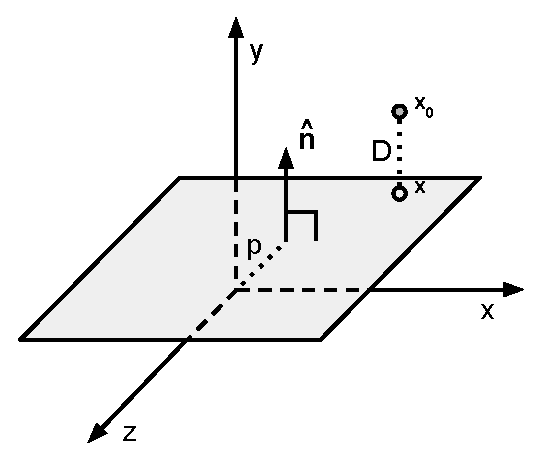
\includegraphics[scale=0.7]{figures/hessian.pdf}
	\caption[Hessian normal form]{
		Visual explanation of the parameters involved in the distance calculation from a point to a plane in Hessian normal form.
	}
	\label{hessian}
\end{figure}

This form can obtained calculating several parameters using the general parametric equation of a plane:

\begin{equation} ax + by + cz + d = 0 \end{equation}

Thanks to this equation we can define the \textit{unit normal vector} $\mathbf{\hat{n}}$:

\begin{equation} \mathbf{\hat{n}} = (n_{x},n_{y},n_{z}) \end{equation}

Being $n_{x}$, $n_{y}$ and $n_{z}$:

\begin{equation} 
\begin{matrix}
n_{x} = \frac{a}{\sqrt{a^2 + b^2 + c^2}}
\\ 
n_{y} = \frac{b}{\sqrt{a^2 + b^2 + c^2}}
\\ 
n_{z} = \frac{c}{\sqrt{a^2 + b^2 + c^2}}
\end{matrix}
\end{equation}

And the constant $p$:

\begin{equation} p = \frac{d}{\sqrt{a^2 + b^2 + c^2}} \end{equation}

Then the Hessian normal form of a plane is:

\begin{equation}\label{eq:hessian} \mathbf{\hat{n}} \cdot \mathbf{x} = -p \end{equation}

Once we have the Hessian normal form parameters (see \autoref{hessian}) and a point $\mathbf{x_{0}}$, the point-plane distance $D$ is given by the following equation:

\begin{equation} D = \mathbf{\hat{n}} \cdot \mathbf{x_{0}} + p \end{equation}

\subsection[Point-cylinder distance]{Point-cylinder distance} 

In the case of the cylinder, the parameters chosen to represent it can be seen in \autoref{cyl_dist}. These parameters will specify an infinite cylinder, that will have to be bound later in order for it to be useful.

\begin{figure}[h]
	\centering
	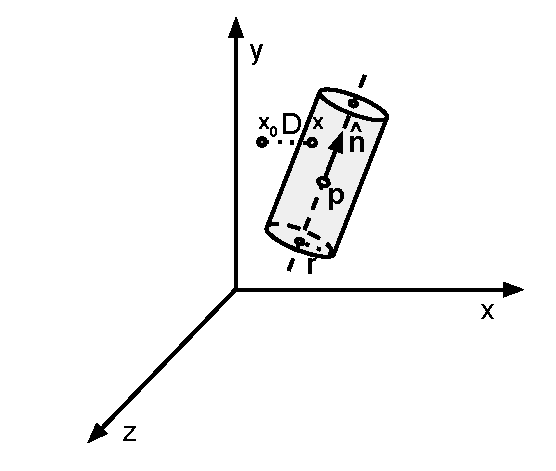
\includegraphics[scale=0.8]{figures/cylinder_dist.pdf}
	\caption[Cylinder parameters]{
		Visual representation of the parameters involved in the point-cylinder distance calculation.
	}
	\label{cyl_dist}
\end{figure}    

The parameter $\mathbf{\hat{n}} = (n_{x},n_{y},n_{z})$ represents the \textit{unit normal vector} of its axis, $\mathbf{p} = (p_{x},p_{y},p_{z})$ a point on its axis and $\mathbf{r}$ its radius. Furthermore, if we define two more unit vectors $\mathbf{\hat{u}}$ and $\mathbf{\hat{v}}$ as a right-handed orthonormal set $\left \{ \mathbf{\hat{u}}, \mathbf{\hat{v}}, \mathbf{\hat{n}} \right \}$, then any point in the cylinder $\mathbf{x}$ can be written as:

\begin{equation} \mathbf{x} = \mathbf{p} + \mathbf{\hat{u}}x + \mathbf{\hat{v}}y + \mathbf{\hat{n}}z \end{equation}

Once we have every parameter and a point $\mathbf{x_{0}}$, we can calculate the distance $D$ with the following equation:

\begin{equation} D = \lVert \mathbf{\hat{n}} \times (\mathbf{x_{0}} - \mathbf{p}) \rVert \end{equation}

\subsection[Point-sphere distance]{Point-sphere distance} 

For spheres, the parameters chosen to represent the estimated primitive can be seen in \autoref{sph_dist}. 

\begin{figure}[h]
	\centering
	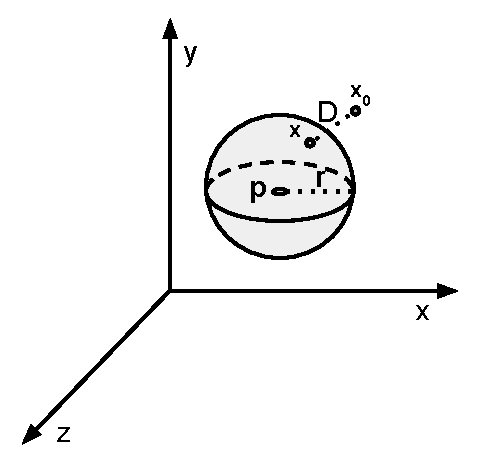
\includegraphics[scale=0.8]{figures/sphere_dist.pdf}
	\caption[Sphere parameters]{
		Visual explanation of the parameters involved in the point-sphere distance calculation.
	}
	\label{sph_dist}
\end{figure}

The parameter $\mathbf{p} = (p_{x},p_{y},p_{z})$ represents the center of the sphere and $\mathbf{r}$ the radius. The Cartesian equation of a sphere centered in $\mathbf{p}$ is:

\begin{equation} (x - p_{x})^2 + (y - p_{y})^2 + (z - p_{z})^2 = \mathbf{r}^2 \end{equation}

When we have every parameter and a point $\mathbf{x_{0}}$, we can calculate the distance $D$ with the next equation:

\begin{equation} D = \lVert \mathbf{x_{0}} - \mathbf{p} \rVert - r\end{equation}

\section[Primitive bounding]{Primitive bounding}

Due to the fact that parametric cylinders and planes are infinite, in order to export them to CAD software we need to bound them. Therefore, we will use the bounding box of the complete dataset to establish these boundaries.

\subsection[Plane bounding]{Plane bounding \label{ss:plane_bound}} 

To bound a plane, we will have to calculate the intersection between the \textit{AABB}\footnote{Axis Aligned Bounding Box} of the scene and a plane. This intersection will yield a three to six vertex polyline\autoref{plane_bound}. 

\begin{figure}[h]
	\centering
	\includegraphics[scale=0.8]{figures/plane_bound.pdf}
	\caption[AABB-plane intersection]{
		Visual representation of a AABB-plane intersection.
	}
	\label{plane_bound}
\end{figure}

In order to obtain the polyline vertices, we will intersect every edge with the plane. This means that a common ray-plane intersection test has to be performed for each edge (see \autoref{ray_plane}). The point of intersection in the plane can be written as in \autoref{eq:hessian} and in the ray can be written as:  

\begin{equation} \mathbf{x} = \mathbf{x_{0}} + t \mathbf{\hat{v}} \end{equation}

\begin{figure}[h]
	\centering
	\includegraphics[scale=0.8]{figures/ray_plane_int.pdf}
	\caption[Ray-plane intersection]{
		Visual representation of a ray-plane intersection.
	}
	\label{ray_plane}
\end{figure}

Being $\mathbf{x_{0}}$ the origin of the ray, $\mathbf{\hat{v}}$ the direction and $t$:

\begin{equation} t = \frac{-(\mathbf{x_{0}} \cdot \mathbf{\hat{n}} + p)}{\mathbf{\hat{v}} \cdot \mathbf{\hat{n}}} \end{equation}

Once all the intersection points have been obtained, they are tested to check if they fall inside the AABB. After this we will have the vertices of the bounded plane ready to be exported.

\subsection[Cylinder bounding]{Cylinder bounding} 

In order to obtain the two points corresponding to the centers of the cylinder bases, we will have to perform a AABB-cylinder intersection test (\autoref{cyl_bound}). To achieve this, we will carry out six ray-plane intersection tests.  

\begin{figure}[h]
	\centering
	\includegraphics[scale=0.8]{figures/cyl_bound.pdf}
	\caption[AABB-cylinder intersection]{
		Visual representation of a AABB-cylinder intersection.
	}
	\label{cyl_bound}
\end{figure}

In this instance, the ray will be the cylinder axis that will be tested against each of the faces of the AABB. This intersection test will be performed in the same manner as in \autoref{ss:plane_bound}, but the ray direction and position instead of being those of the AABB, will be those of the cylinder axis (see \autoref{cyl_ray_plane}). The planes against which the ray has to be tested will be the faces of the AABB.

\begin{figure}[h]
	\centering
	\includegraphics[scale=0.8]{figures/cyl_ray_plane.pdf}
	\caption[Cylinder axis-plane intersection]{
		Visual representation of a ray-plane intersection with the cylinder axis as ray.
	}
	\label{cyl_ray_plane}
\end{figure}

Once we have all the intersection points, we will have more than two intersection points. That is why one extra step is needed to bound the cylinder, the sorting of the points according to the distance to the AABB center $\mathbf{c}$:

\begin{equation} D = \lVert \mathbf{x} - \mathbf{c} \rVert \end{equation}

Finally, the two cylinder bases will be the two closest points to the AABB center. This is the last step necessary to get the cylinder ready for exportation.

\section[Results]{Results}

To test the different algorithms we will compare the estimation times achieved with them. We will first test a 3038 point sample, from which we want to estimate a plane (see \autoref{ransac_table_3k}).

\begin{table}[h]
	\begin{center}
    \begin{tabular}{cc}
    \toprule
    Algorithm & Time(ms) \\
    \midrule
    RANSAC & 71.886 \\
    MSAC & 71.8124 \\
    MLESAC & 106.342 \\
    PROSAC & 71.641 \\
    RRANSAC & 71.5368 \\
    \bottomrule
    \end{tabular}
    \end{center}
	\caption[RANSAC testing results]{
		Table showing the estimation times achieved with each algorithm.
	}
	\label{ransac_table_3k}
\end{table}

As we can see, the fastest algorithm is RRANSAC. Although, we have to keep in mind that the most robust algorithms are MSAC and MLESAC after thorough testing. In light of these results, the chosen method to estimate primitives in ToView was MSAC. The following segmentations were performed using the aforementioned algorithm: \autoref{plane_seg}, \autoref{cylinder_seg} and \autoref{sphere_seg}.

\begin{figure}[h]
	\centering
	\includegraphics[scale=0.4]{figures/seg_plane.png}
	\caption[Plane segmentation test]{
		Segmented plane using ToView.
	}
	\label{plane_seg}
\end{figure}

\begin{figure}[h]
	\centering
	\includegraphics[scale=0.4]{figures/seg_cyl_r.png}
	\caption[Cylinder segmentation test]{
		Segmented cylinder using ToView.
	}
	\label{cylinder_seg}
\end{figure}

\begin{figure}[h]
	\centering
	\includegraphics[scale=0.4]{figures/seg_sph.png}
	\caption[Sphere segmentation test]{
		Segmented sphere using ToView.
	}
	\label{sphere_seg}
\end{figure}





	% INCLUIMOS LOS AP�NDICES...
        %\appendix
	%\include{tfg_appendix_010}
%         \include{tfg_appendix_020}

	%Primero hay que compilar el bibtex para que salga.
	% INCLUIMOS LA BIBLIOGRAF�A...
	\nocite{*}	% Se usa para indicar en la bibliograf�a las referencias no citadas.
	\bibliography{tfg_biblio}
	\bibliographystyle{alpha}

\end{document}

